%%%%%%%%%%%%%%%%%%%%%%%%%%%%%%%%%%%%%%%%%%%%%%%
%
% Template for Master degrees
% DISI - Dipartimento di Ingegneria e Scienza dell’Informazione
% DISI - Department of Information Engineering and Computer Science
%
% update 2020-08-30
%
% To generate pdf 
% pdflatex __filename__.tex
% bibtex __file_name__.aux
% pdflatex __file_name__.tex
% pdflatex __file_name__.tex
%
%%%%%%%%%%%%%%%%%%%%%%%%%%%%%%%%%%%%%%%%%%%%%%%

% 2 side format
\documentclass[epsfig,a4paper,11pt,titlepage,twoside,openany]{book}
\usepackage{epsfig}
\usepackage{plain}
\usepackage{setspace}
\usepackage[paperheight=29.7cm,paperwidth=21cm,outer=1.5cm,inner=2.5cm,top=2cm,bottom=2cm]{geometry} % layout setting
\usepackage{titlesec} % custom setup title of chapter

% Support for accented letters
\usepackage[utf8]{inputenc}

% Line spacing
\singlespacing

% Better URL formatting and break on hyphens
\usepackage[hyphens]{url}
\usepackage[hidelinks]{hyperref}

% "Continuous" footnote numbers
\counterwithout{footnote}{chapter}

% Code blocks
\usepackage{minted}

% Fix quotes. Should be kept last or it complains
\usepackage [english]{babel}
\usepackage [autostyle, english = american]{csquotes}
\MakeOuterQuote{"}

\newcommand{\ffmpeg}{\texttt{ffmpeg}}

\begin{document}

  % No page number
  \pagenumbering{gobble} 
  \pagestyle{plain}

\thispagestyle{empty}

\begin{center}
  \begin{figure}[h!]
    \centerline{
\psfig{file=res/marchio_unitrento_colore_it_202002.eps,width=0.6\textwidth}}
  \end{figure}

  \vspace{2 cm} 

  \LARGE{Department of Information Engineering and Computer Science\\}

  \vspace{1 cm} 
  \Large{Master's Degree in\\
    Computer Science
  }

  \vspace{2 cm} 
  \Large\textsc{Final Dissertation\\} 
  \vspace{1 cm}
  %\Huge\textsc{IMPROVING LOW-LATENCY ADAPTIVE BITRATE LIVE VIDEO STREAMING OVER HTTP/3}
  \Huge\textsc{Improving low-latency adaptive bitrate live video streaming\\over HTTP/3}
  %\Large{\it{Sub-title (optional)}}


  \vspace{2 cm} 
  \begin{tabular*}{\textwidth}{ c @{\extracolsep{\fill}} c }
  \Large{Supervisor} & \Large{Student}\\
  \Large{Fabrizio Granelli}& \Large{Matteo Contrini}\\
  \end{tabular*}

  \vspace{2 cm} 

  \Large{Academic year 2021/2022}
  
\end{center}



  \clearpage

  \thispagestyle{empty}

\begin{center}
  {\bf \Huge Acknowledgements}
\end{center}

\vspace{4cm}


\emph{
  ...thanks to...
}

  \clearpage
  \pagestyle{plain} % no heading, footer with centered page number

  
  % page number with Arabic format
  \mainmatter

    % index
    \tableofcontents
    \clearpage


    % group to define space between chapters
    \begingroup
      % no page break between chapters
      % override clear page commands
      %\renewcommand{\cleardoublepage}{}
      %\renewcommand{\clearpage}{}

      \titlespacing*{\chapter}{0pt}{0.59in}{0.02in}
      \titlespacing*{\section}{0pt}{0.20in}{0.02in}
      \titlespacing*{\subsection}{0pt}{0.10in}{0.02in}
      
      % summary / abstract
      \chapter*{Abstract} % no number
\label{abtract}

\addcontentsline{toc}{chapter}{Abstract} % add to index

Video streaming over the Internet has become increasingly popular in recent years and now accounts for more than 50\% of total traffic. One of the main challenges video developers have to tackle is providing a user experience that is as smooth as possible. In live video streaming, low-latency in particular, the problem is especially challenging and requires finding a trade-off between reducing the probability of video freezes (rebuffering) and keeping a high video quality.

In this thesis, we first develop a testbed to evaluate the performance of adaptive bitrate video streaming technologies. We then run some emulations and experiment with real-word network datasets to analyze how existing solutions behave. We find that some configurations show suboptimal behavior and propose some improvements based on that. The main proposed solution, which takes advantage of HTTP/3 features and modern browser APIs such as WebCodecs and WebAssembly, shows that it is possible to greatly reduce playback stalls and to provide a smooth playback experience with stable live latency, as the experimental results show.

\newpage



%% The first chapter of the final thesis must contain a summary of a 
%% maximum length of 3 pages, introducing the context and motivations,
%% resuming the problem faced by the student, the techniques used for the
%% investigation and the reached outcomes.
%% If the final thesis is developed in collaboration with other students,
%% the personal contribution of the student has to be underlined.
  
      
      %%%%%%%%%%%%%%%%%%%%%%%%%%%%%%%%
      % chapters
      %
      % \input or \include
      %
      \chapter{Introduction}
\label{cha:intro}

During the last decade, the usage of \textbf{online video streaming} has exploded. From sports to entertainment, the market has seen strong growth in the past few years and video streaming now accounts for more than half of Internet traffic.\cite{cisco2019}

\textbf{Live events streaming} in particular is becoming increasingly relevant, with a 15-fold growth in just five years, according to statistics. This is in part due to the effect of the pandemic, through which many organizations started to live stream events and kept doing it, and in part due to a more general shift from traditional broadcasting means such as DVB-T (digital terrestrial), cable TV and satellite to Internet streaming. A special category of live streaming is \textbf{low-latency streaming}, as we will see, which is particularly relevant for use cases such as sporting events, gaming, and live news coverage.

In this chapter, we will briefly introduce the context of our work, namely, how modern video streaming works and what the main challenges are. We will then present how these challenges are usually tackled and why we believe that a different point of view could be needed to provide a satisfying user experience to viewers. Finally, we will introduce our proposal that we believe improves the live streaming quality of experience.

\section{Live video streaming and latency}
\label{sec:intro/live}

Video streaming is typically divided into two main categories: on-demand and live. With \textbf{video on demand} (VoD), we typically mean prerecorded content that can be watched by the user at any time, while \textbf{live} refers to events that are produced and transmitted as they happen.

When considering the live streaming scenario, \textbf{latency} is an important factor. For example, in sporting events viewers expect to see the action as soon as possible without delays, especially if they are able to compare the live stream with other broadcasting means such as digital terrestrial.

According to Wowza, a leading company in the streaming industry, a live stream can be considered \textbf{low latency} if it has a latency of less than 5 seconds.\footnote{\url{https://www.wowza.com/low-latency}} However, latency can be defined in many ways. A typical definition is the glass-to-glass (or end-to-end) latency, computed as the time it takes for a video frame captured by a camera (the "glass") to be shown on the screen of the user (the other "glass"). Other times, the latency is measured from the moment the video frame is \textit{ingested}, which in practice means the moment when it is fed as input to the video transcoder.

\section{Network constraints}
\label{sec:intro/networks}

Video streaming over the public Internet faces the problem of \textbf{slow or congested networks}. Bandwidth (or throughput) could in fact be very low or oscillating, creating situations where there is not enough bandwidth to play the video stream smoothly. This is particularly challenging with live video streaming, where we cannot rely on the fact that the video is already available and therefore it cannot be buffered in advance by the player.

Although modern compression standards achieve significant compression ratios, leading to bitrates usually below 10 Mbps even for high-resolution content at good quality, not all networks are always able to provide such bitrates reliably.

In fact, while modern access networks such as fiber optics and 4G/5G can be quite reliable and provide a high throughput, Internet connectivity is still far from being perfect. As an example, very high capacity networks are still not dominant in most countries. Mobile networks coverage can be problematic too, and Wi-Fi connectivity can be unstable due to interferences and limitations of the wireless protocols.

An additional source of issues that is often overlooked is the Internet Service Provider network, whose backhauling infrastructure needs to be sized properly to avoid congestion. Interconnections with CDNs and other providers are also very important, as they can become congested during peak hours if capacity upgrades are not properly planned in advance.

These issues led to the development of a number of video streaming technologies, among which \textbf{Adaptive Bitrate Streaming} protocols based on HTTP are nowadays considered the de facto standard in the industry.\cite{bitmovin}

\section{Adaptive bitrate technologies}
\label{sec:intro/technologies}

The core idea of \textbf{Adaptive Bitrate Streaming} (ABR) is to have video content encoded in multiple renditions, or variants, with different resolutions and bitrates. The set of video renditions and their parameters constitute a \textit{bitrate ladder}. Video players use different techniques to understand which rendition is the best for the current device and network conditions, and thus \textit{adapt} accordingly. The aim is to provide uninterrupted playback at the best possible quality.

The two most common protocols for adaptive streaming are \textbf{Apple HLS} (HTTP Live Streaming) and \textbf{MPEG-DASH} (Dynamic Adaptive Streaming over HTTP). As the names suggest, both work over HTTP and are conceptually similar.

They require video content to be encoded in short video segments (no more than a few seconds) so that players can switch rendition at segment boundaries. Bitrate adaptation algorithms should find a trade-off between reducing the probability of video freezes (rebuffering) and keeping a high video quality level, but neither HLS or DASH mandate how players should choose the bitrate for the next segment. Multiple approaches are possible, as we will see in more detail in the following chapters.

An important benefit of using HTTP for video streaming is that it makes it easy for streaming platforms to scale, thanks to the widespread availability of \textbf{Content Delivery Networks} (CDN) and their global distribution networks.

\section{Challenges in live video streaming}
\label{sec:intro/challenges}

Both HLS and DASH support \textbf{live streams}. They do so by making new video segments available as soon as they are encoded.

Delivering live streams introduces a new category of challenges for video players, which need to find a trade-off between stream reliability and lower latency. In fact, lowering latency usually means keeping a smaller buffer of media data on the client, with the disadvantage that rate adaptation algorithms might not be able to react timely to network fluctuations. If video segments cannot be loaded in time, this can cause rebuffering.

\section{A different live user experience}
\label{sec:intro/experience}

When a live video streaming setup struggles to adapt to network conditions, the most noticeable effect is \textbf{rebuffering}. The playback gets stuck while the player tries to complete the download of the next video segment, and the \textbf{latency tends to grow}. As a consequence, playback will lag behind the live event and users will receive the action late, possibly by even tens of seconds.

This kind of experience is \textbf{different from other broadcasting mechanisms}. For example, digital terrestrial and satellite do not have the concept of buffering: if the video signal is not good enough, video and/or audio are temporarily unavailable while the signal recovers, but no latency is introduced, i.e. viewers always see the live action with a fixed delay independently from the signal quality.

Adaptive streaming research has been mostly focused on avoiding empty buffers as much as possible, although in low-latency scenarios completely avoiding rebuffering is a very hard task. Instead, there are methods that can be integrated in an adaptive streaming setup so that the linear TV experience that viewers are already used to can also be replicated in video streaming. Although subjective, it would likely result in a better Quality of Experience (QoE).

\section{Contributions and results}
\label{sec:intro/contributions}

In this work, we first develop a \textbf{testbed} for experimenting with HTTP-based live streaming protocols. We then use the testbed to evaluate the performance of existing live streaming protocols such as HLS and DASH with different configurations and HTTP versions. One of the things we observe is that streaming over \textbf{HTTP/3}, a recent version of HTTP based on the QUIC transport protocol, shows an unexpected and suboptimal behavior in terms of prioritization of requests. This is especially evident in comparison to HTTP/1.1 and HTTP/2.

Among other improvements, we therefore introduce a modified version of the \hlsjs{} library that takes advantage of HTTP/3 features to \textbf{override the default prioritization strategy} of HTTP responses. By giving priority to audio segment requests, we get closer to a user experience where the lack of video buffer does not cause playback stalls.

The next step is to implement a strategy we call \textbf{segment dropping}: when a video segment is needed for playback but is still being loaded, we interrupt the request and thus reset the underlying QUIC stream, freeing bandwidth that would otherwise be used to download a video segment that is already outdated.

The dropped segment needs to be replaced with a placeholder that we call \textbf{filler segment}. This segment is dynamic and generated on the fly in the frontend, taking advantage of the WebCodecs API and WebAssembly.

The experimental results show that this solution almost eliminates video playback stalls, providing smooth playback of the audio track even when the video could not be loaded. In this way, even when the video rate adaptation algorithm is slow to react to new network conditions, a smooth user experience is preserved.

\section{Thesis structure}
\label{sec:intro/structure}

This thesis is organized as follows. In \textbf{Chapter \ref{cha:bg}}, we introduce the main concepts and technologies surrounding video compression and streaming over HTTP. In \textbf{Chapter \ref{cha:testbed}}, we introduce the testbed setup that we developed to evaluate the performance of streaming protocols. In \textbf{Chapter \ref{cha:eval}}, we show the results of the analysis of some experiment runs that show suboptimal behavior. In \textbf{Chapter \ref{cha:improvements}}, we propose some improvements to the live streaming user experience and show the results of the implementation of a modified version of HLS. Finally, in \textbf{Chapter \ref{cha:conclusions}} we acknowledge some limitations of our work and mention a few ideas that are left for future work.


      \chapter{Background}
\label{cha:bg}

% TODO


\section{Video compression concepts}
\label{sec:bg/compression}

Video is known to be one of the heaviest types of content to be stored and transmitted. Since treating uncompressed video is unfeasible, video compression or video coding formats have been developed and standardized over the years, with multiple implementations (\textbf{codecs}) being released. The objective of video codecs is to limit the output data rate, measured in bits per second, while trying to maintain a perceptually good video quality.

The process of compressing a video is known as \textbf{encoding} and is carried out by an encoder. When a video file is already encoded in a video coding format and needs to be encoded in another, we often use the term \textbf{transcoding}.

In this section, we will go through the main techniques that are used by most video coding standards.

\subsection{RGB vs Y'CbCr}
\label{sec:bg/compression/ycbcr}

The most basic form of compression can be obtained by converting individual pictures representing the video to a \textbf{color space} that better exploits human vision characteristics and then applying compression of some of the components in the new color space.

A very common color space family used in digital video and images is \textbf{Y'CbCr}, sometimes improperly called YUV (which relates to the analog domain), which exploits the fact that the human vision system is much more sensitive to light variations (brightness) than to color. The Y'CbCr color space decomposes the color information of a pixel into three components:

\begin{itemize}
    \item \textbf{Y'}: the luminance, representing the brightness of the image;
    \item \textbf{Cb}: the blue chroma component, representing a projection of the blue color;
    \item \textbf{Cr}: the red chroma component, representing a projection of the red color.
\end{itemize}

This approach is different from the common RGB (Red Green Blue) color space, where the luminance is not isolated from the color components, and allows compression to be applied more effectively through the \textbf{chroma subsampling} technique.

Chrome subsampling refers to the practice of reducing the resolution of the chroma components while keeping the luminance at full resolution. Since our eyes are less sensitive to color than to brightness, we can reduce the color resolution by even 75\% with almost no perceptual impact on quality.

% sources from LT

The vast majority of digital video that can be found on the Internet or that is transmitted through digital television is compressed with the Y'CbCr 4:2:0 color space, the most common format for nonprofessional content. In Y'CbCr 4:2:0, the luminance component (Y) is encoded at full resolution, while the chroma components are stored at 1/4 of the resolution, that is, instead of storing 8 chroma samples for every 8 pixels we only keep 2, as shown in Figure X.

% figure from LT

When compared to a typical 8-bit RGB image (equivalent to Y'CbCr 4:4:4, i.e. no subsampling), requiring 24 bits per pixel, a Y'CbCr 4:2:0 image requires only 12 bits per pixel, resulting in a 50\% saving with very similar perceived quality. When using tools like \texttt{ffmpeg}, Y'CbCr 4:2:0 is often called \texttt{yuv420p} or similar.

\subsection{Inter-frame and intra-frame compression}
\label{sec:bg/compression/intra-inter}

The major video coding standards released since the early 1990s are based on a \textbf{hybrid codec model} that exploits both temporal and spatial redundancy of videos to achieve high compression ratios.

Temporal compression, or \textbf{inter-frame compression}, relies on the fact that there is usually a high similarity between consecutive video frames. On the other hand spatial compression, or \textbf{intra-frame compression}, exploits the fact that pixels that are close to each other within a picture are usually highly correlated.

Video codecs (en\textbf{co}der/\textbf{dec}oder) are implementations of video coding standards that are able to convert the input video into a coded version in a way that is reversible, i.e. such that the decoder can reconstruct the original video with some approximation. Encoders should output a compressed representation that is as efficient as possible while trying to preserve the fidelity of the original video.

\begin{figure}[h]
	\centering
	
	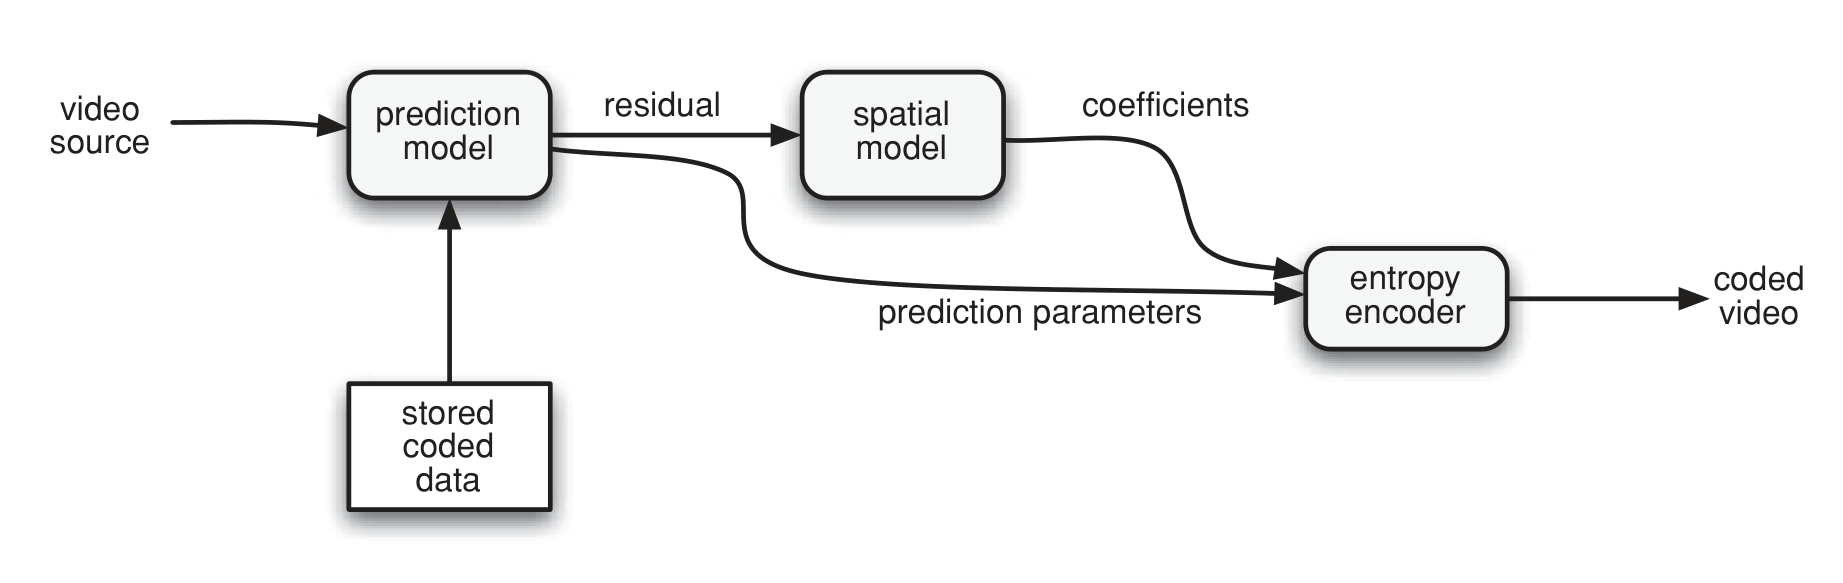
\includegraphics[width=\textwidth]{res/hybrid_codec_high_level.png}
	
	\caption{High-level hybrid codec architecture.\cite{h264}}
	\label{fig:codec_highlevel}
\end{figure}

In general, a hybrid video codec works in three phases:\cite{h264}

\begin{itemize}
    \item \textbf{Prediction model}: exploits spatial or temporal redundancy by producing a prediction of the current frame (or block of a frame) being analyzed, by looking at a previous reference frame or at other parts of the same frame. The outputs of this phase are a \textbf{residual frame}, which is the difference between the actual frame and the predicted frame, and the parameters that define how the prediction was obtained. By encoding only the residual and the parameters we can basically store only the "error" of the prediction and greatly reduce the amount of data that needs to be coded. The prediction can be obtained in two ways:
        \begin{itemize}
            \item \textbf{Temporal prediction}: in its most basic form, the prediction is the difference between the current frame and a previous (or future) reference frame. In practice, we also need to take into account the motion that occurs between frames by running a \textbf{motion estimation} algorithm that for each block\footnote{Blocks are small regions of pixels.} in the current frame finds the best matching block in the reference frame. The \textbf{motion-compensated block} becomes the prediction used to calculate the residual, which becomes the output of the prediction phase together with the \textbf{motion vectors} that explain how the prediction block was obtained (i.e. how it "moved" with respect to the reference frame).
            \item \textbf{Spatial prediction}: when encoding a block of the image, a prediction of the pixel values of the block is first calculated by looking at neighboring pixels. Statistically, pixels close to each other are expected to be similar due to spatial redundancy. Usually, this means looking at the pixels on the left and/or top edges of the block. The predicted block is then subtracted from the current block to obtain a \textbf{residual block}, which is passed onto the next phase together with the information that tells how the prediction of the block was obtained.
        \end{itemize}
        
    \item \textbf{Spatial model}: in most codecs, this phase consists in compressing the residual frame through transform and quantization steps, followed by encoding of the coefficients.
        \begin{itemize}
            \item The \textbf{transform} step often consists in applying the \textbf{Discrete Cosine Transform} (DCT) to transform the blocks in the frequency domain. The output of the DCT is a matrix of coefficients which can be used to faithfully reconstruct the original block, although without achieving any compression.
            \item In the \textbf{quantization} step, coefficients that have insignificant impact, such as values that are close to zero, are discarded, enabling to represent the original block with some approximation by storing a smaller number of DCT coefficients (the non-discarded ones). In the decoder, the subset of coefficients can then be fed into the IDCT (the inverse of the transform), obtaining a reconstruction of the original block. The fidelity of the reconstruction depends on how strong the quantization step was, i.e. on the \textbf{quantization parameter} (QP).
            \item After quantization, the remaining coefficients are reordered through a \textbf{zigzag scan} of the matrix, making sure that the most significant coefficients are at the beginning of the sequence (a typical property of the DCT) and then encoded through \textbf{Run-Level Encoding} (RLE).
        \end{itemize}
     
    \item \textbf{Entropy coding}: in this phase all the information collected in previous phases, including quantized coefficients, quantization parameters, and motion vectors, is encoded in a bit stream. To exploit the statistical redundancy of symbols in the data, techniques like \textbf{Variable-Length Coding} (VLC), such as Huffman coding, or arithmetic coding and \textbf{Context-aware Arithmetic Encoding} (CAE) are used, achieving further compression.
\end{itemize}

\begin{figure}[hb]
	\centering
	
	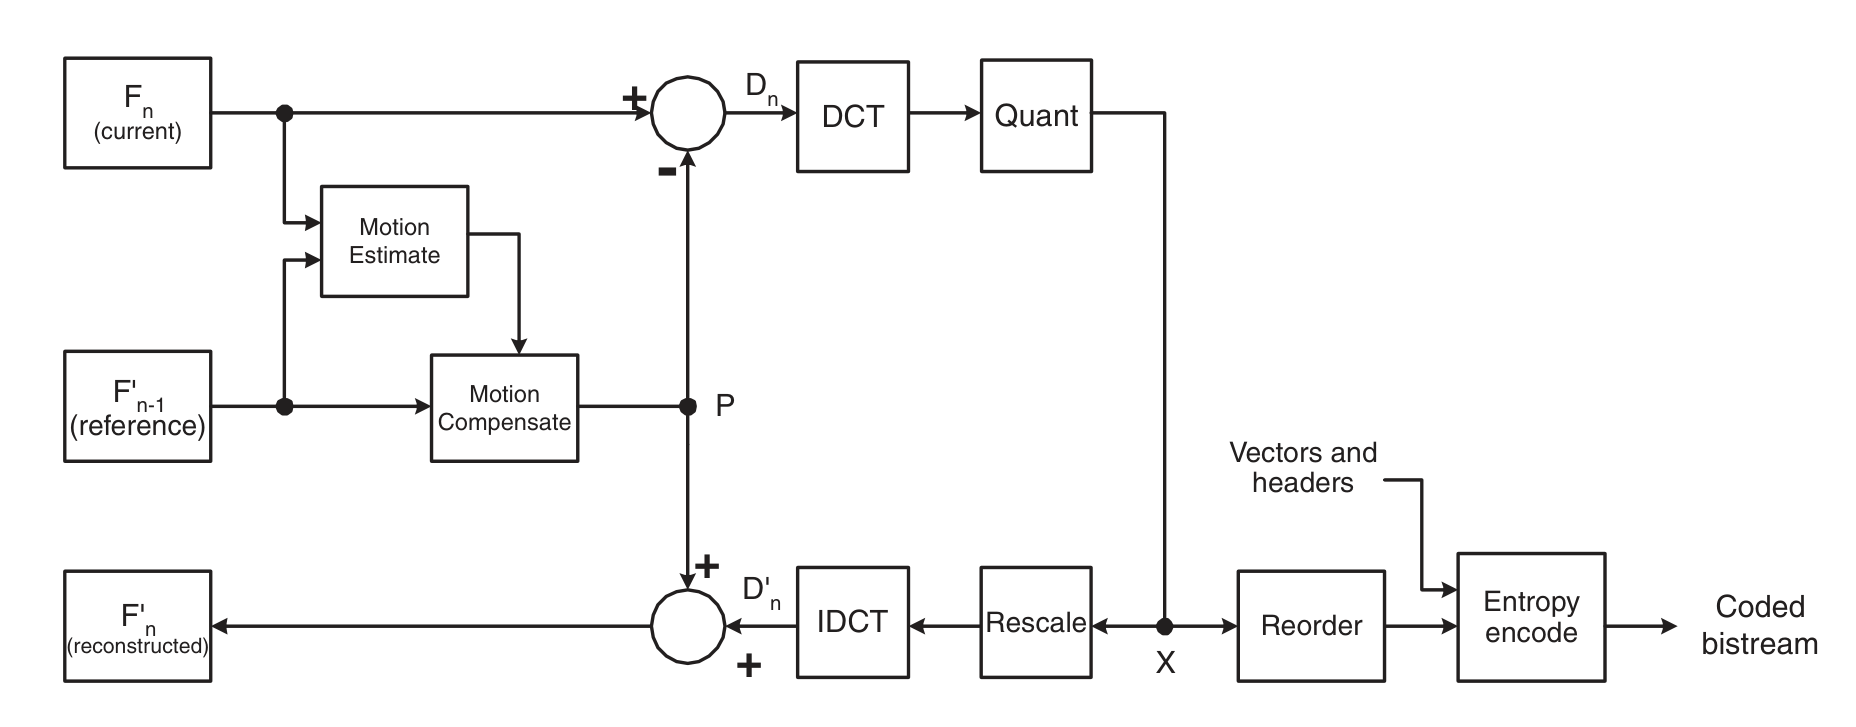
\includegraphics[width=\textwidth]{res/hybrid_codec_detailed.png}
	
	\caption{Detailed hybrid codec architecture.\cite{h264}}
	\label{fig:codec_detailed}
\end{figure}

%The transform converts the samples into another domain in which they are represented by transform coefficients. The coefficients are quantized to remove insignificant values, leaving a small number of significant coefficients that provide a more compact representation of the residual frame. The output of the spatial model is a set of quantized transform coefficients.

%The parameters of the prediction model, i.e. intra prediction mode(s) or inter prediction mode(s) and motion vectors, and the spatial model, i.e. coefficients, are compressed by the entropy encoder. This removes statistical redundancy in the data, for example representing commonly occurring vectors and coefficients by short binary codes. The entropy encoder produces a compressed bit stream or file that may be transmitted and/or stored. A compressed sequence consists of coded prediction parameters, coded residual coefficients and header information. The video decoder reconstructs a video frame from the compressed bit stream. The coefficients and prediction parameters are decoded by an entropy decoder after which the spatial model is decoded to reconstruct a version of the residual frame. The decoder uses the prediction parameters, together with previously decoded image pixels, to create a prediction of the current frame and the frame itself is reconstructed by adding the residual frame to this prediction.

The output of a hybrid video encoder is a \textit{bit stream} (or \textit{bitstream}), i.e. a compressed sequence of coded residual coefficients and other parameters. The decoder applies the same process inversely to reconstruct the original video frames, with some approximation.

\subsection{Frame types and GOP}
\label{sec:bg/compression/gop}

As we have seen, the prediction model can be based on temporal (inter-frame) prediction or spatial (intra-frame) prediction. The type of prediction that is used and which reference frames are used for the prediction determine the type of frame. In particular:

\begin{itemize}
    \item \textbf{I-frames} (\textit{Intra-frames}) are frames that do not require any other frames to be decoded and are thus compressed only by intra-frame prediction.
    \item \textbf{P-frames} (\textit{Predicted frames}) are frames that can reference other previous frames when performing temporal prediction. Depending on the codec, a frame can reference one or more previous frames.
    \item \textbf{B-frames} (\textit{Bi-directional predicted frames}) are frames that can reference both previous and future frames as reference frames in temporal prediction. They are more computationally expensive to encode, but are usually the most compressible ones.
\end{itemize}

Because of inter-frame dependencies, the display order of frames is very often different from the decoding order.

Depending on the type of frames that are used to encode a video sequence, different \textbf{prediction structures} can be obtained. For example, low delay applications could use a structure like the one in figure \ref{fig:codec_gop1}, where only I-frames and P-frames are used and P-frames always reference the previous frame. I-frames should be inserted into the stream periodically to allow more efficient random access (\textit{seeking}). Another reason is that in some cases scene cuts might justify the use of an I-frame instead of a P-frame, depending on how drastic the scene change is.

\begin{figure}
	\centering
	
	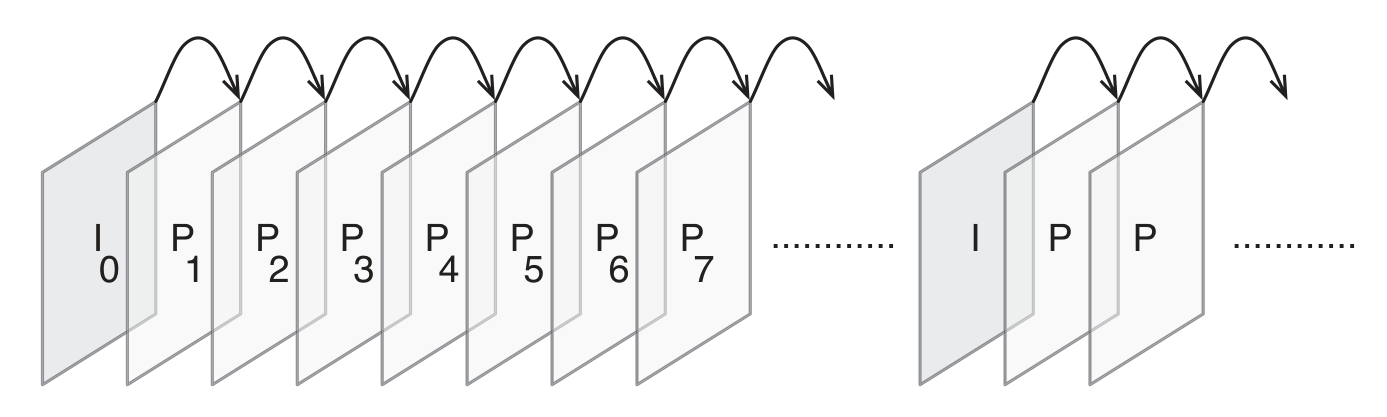
\includegraphics[width=0.9\textwidth]{res/gop1.png}
	
	\caption{Simple GOP structure with no B-frames.}
	\label{fig:codec_gop1}
\end{figure}

Most of the time, the arrangement of the frames is much more complex and is usually defined by a \textbf{Group of Pictures (GOP)} structure, as seen in Figure \ref{fig:codec_gop2}. A GOP always starts with an I-frame and is most of the time \textit{closed}, which means that it is independent from previous and future GOPs. As a consequence, in a closed-GOP scenario the decoder does not need access to previous of future GOPs to be able to decode frames in the current GOP.

The structure of a GOP can be summarized as a string sequence, like \texttt{IBBPBBPBBPBBI}, or through two numbers, \texttt{M} and \texttt{N}, that respectively determine the distance between P-frames, and the GOP size. For example, the structure in Figure \ref{fig:codec_gop2} can be expressed as \texttt{M=3, N=12}.

\begin{figure}
	\centering
	
	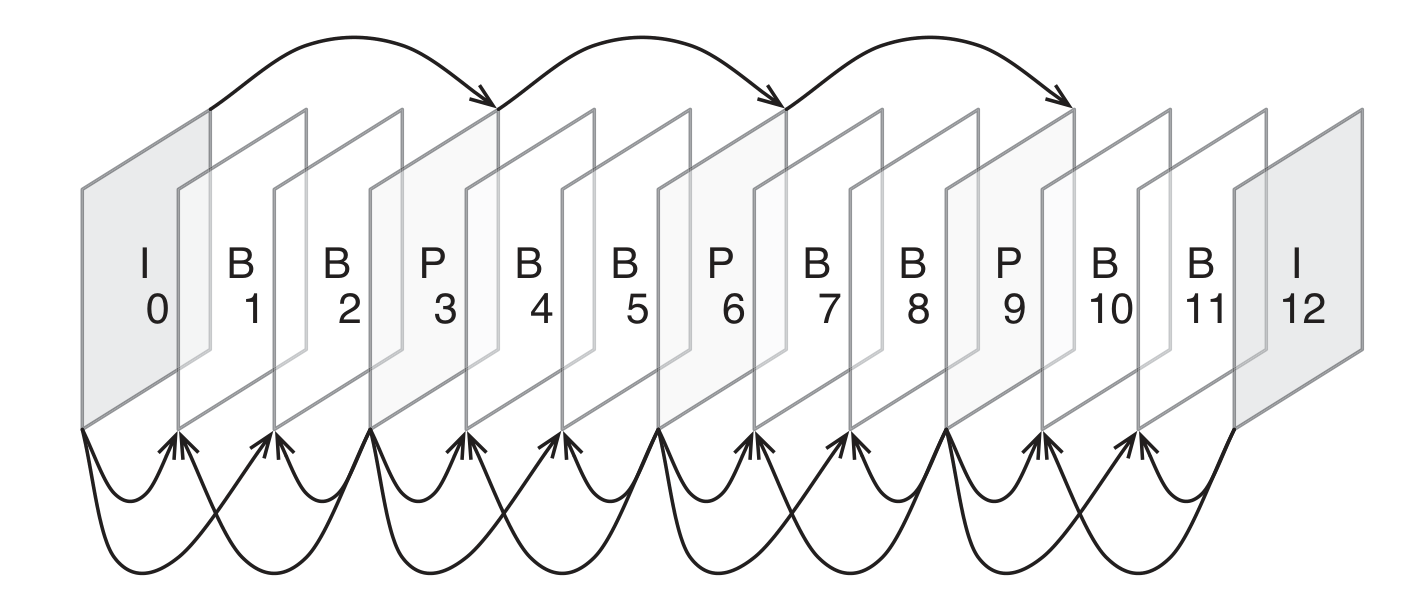
\includegraphics[width=0.8\textwidth]{res/gop2.png}
	
	\caption{Typical GOP structure, \texttt{M=3, N=12}.}
	\label{fig:codec_gop2}
\end{figure}

\subsection{Popular video coding formats}
\label{sec:bg/compression/codecs}

The dominant video coding standard is currently \textbf{H.264}, sometimes referred to as \textit{Advanced Video Coding} (AVC) or \textit{MPEG-4 Part 10}, developed by a joint team of the ITU (Video Coding Experts Group) and ISO (Moving Picture Experts Group, or \textbf{MPEG}). H.264 was first standardized in 2003, nevertheless it is estimated that H.264 is still used today by more than 80\% of the companies in the industry, thanks to its good performance (both in terms of compression and encoding/decoding efficiency) and the accessible royalties structure.\cite{bitmovin}

It is worth noting that the H.264 standard only defines the format and syntax of the H.264 bitstream and how to decode it, but it does not specify how to actually encode a video. This is why the term \textit{codec} should be only used to refer to the actual software implementations of H.264, which typically include both an encoder and a decoder.

The successor of H.264, first published in 2013, is \textbf{H.265}, also named \textit{High Efficiency Video Coding} (HEVC) or \textit{MPEG-H Part 2}, delivering 25\% to 50\% better compression at the same bitrate when compared to H.264. It is especially suitable for high-resolution content like 4K UHD, but it struggled to reach wide adoption because of the complex and expensive royalties structure that slowed down hardware support.\cite{hevcroyalties}

Apart from the H.26x family of formats, Google released the royalty-free \textbf{VP8} in 2008, followed by \textbf{VP9} in 2012. Thanks to Google controlling a large fraction of the browsers market share and the YouTube streaming platform, VP9 became a popular alternative to H.264, often delivering better video compression ratios with comparable quality.

% TODO: sources

The successor to VP9 was incorporated into \textbf{AV1} (first released in 2018), the royalty-free video format developed by the \textit{Alliance for Open Media} (AOMedia), an initiative backed by large companies such as Google, Apple, Meta, Microsoft, Amazon, Netflix, Cisco, NVIDIA, Intel, among others.\footnote{\url{https://aomedia.org/membership/members/}} AV1 is much more complex than H.264 and achieves up to 50\% better compression when compared to H.265, making it especially suitable for high resolution content such as 4K UHD or 8K UHD. The downside of AV1 is that since it is quite complex, codec implementations are often prohibitively expensive to run in software, thus requiring hardware support, an effort that can require quite a few years.\cite{av1}

\subsubsection{H.264}
\label{sec:bg/compression/codecs/h264}

\begin{figure}
	\centering
	
	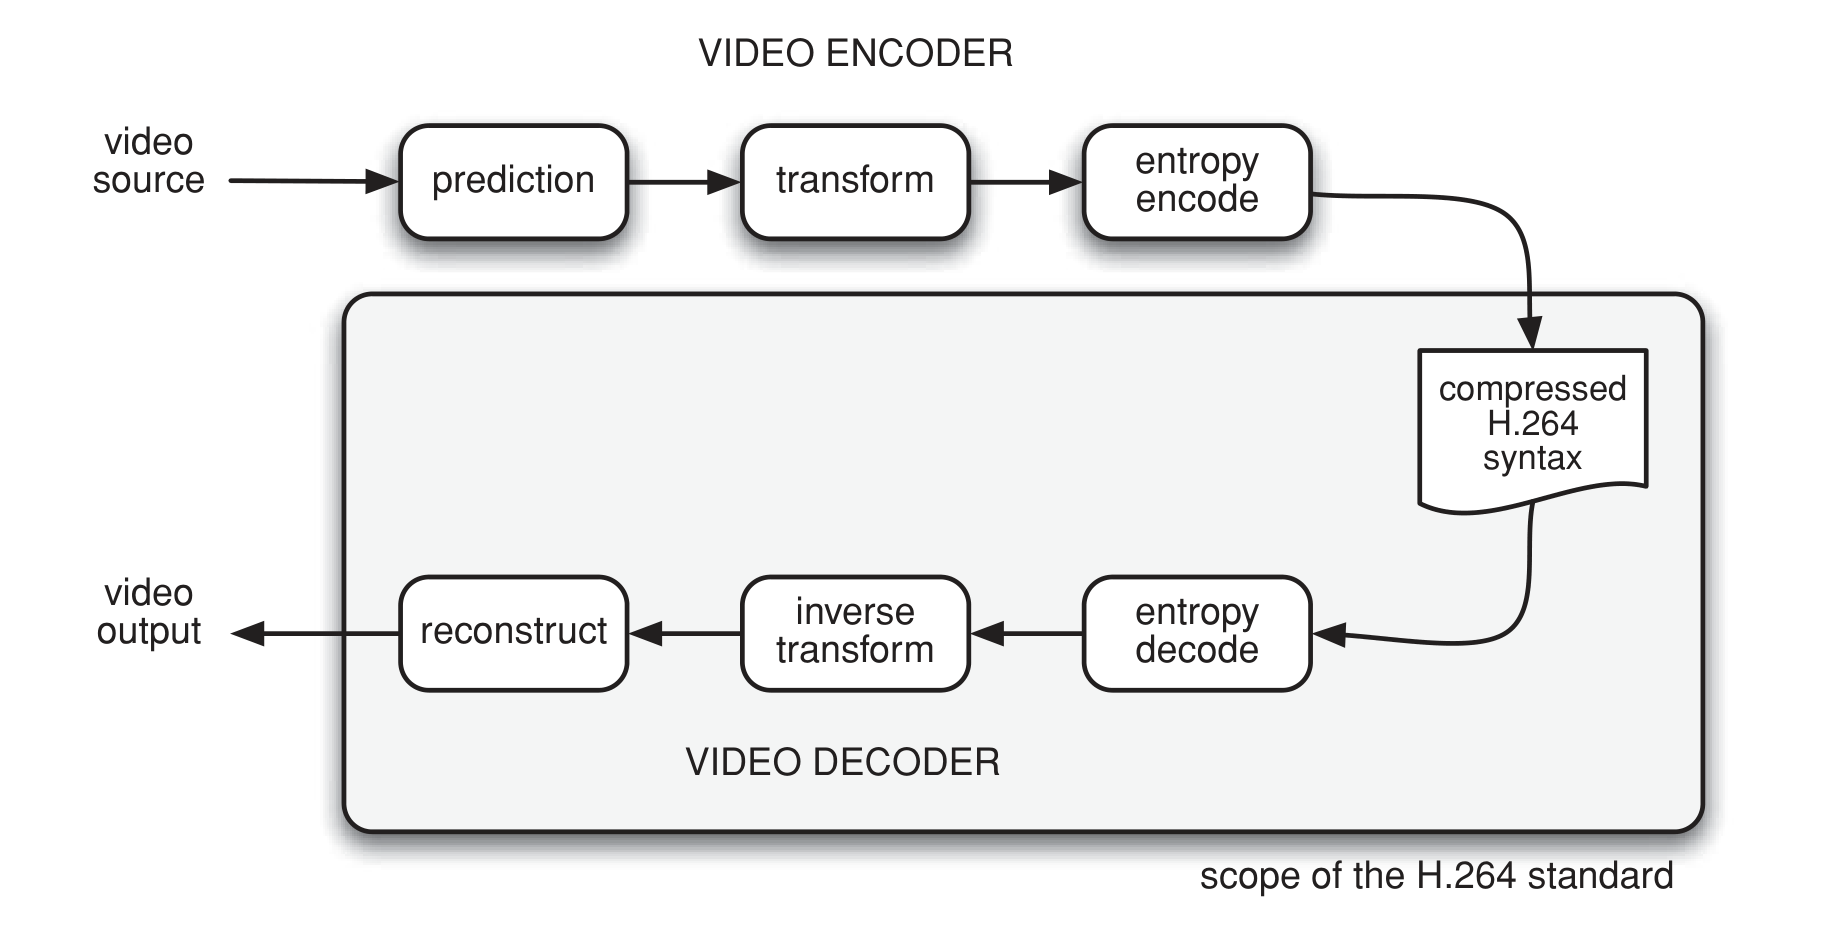
\includegraphics[width=0.8\textwidth]{res/h264_scope.png}
	
	\caption{The scope of the H.264 standard.}
	\label{fig:h264_scope}
\end{figure}

As we have seen, H.264 is still the dominant video format in the industry. Since the standard only covers the decoding part of the codec, as shown in Figure \ref{fig:h264_scope}, many codec implementations have been released, achieving different compression results. One of the most popular H.264 encoders is \texttt{x264}, which is open source and software-based, typically scoring as the best speed/quality trade-off in H.264 codec comparisons.\cite{msu2021} \texttt{x264} is also the default codec in \texttt{ffmpeg}, a very popular tool for video and audio manipulation and compression.

H.264 is based on the hybrid codec model we have introduced earlier. Frames are divided into 16x16 pixels \textbf{macroblocks} (MB), on which the prediction model is applied. Macroblocks can be split into partitions that can be as small as 4x4 pixels (not necessarily square), so that the same macroblock can reference different macroblocks possibly in different reference frames.

In H.264, the transform is an approximation of the DCT and can be applied on 4x4 or 8x8 blocks. Quantization can be controlled by the QP parameter, or step size, which ranges from 0 to 51 and is usually adjusted automatically by the encoded depending on the input configuration. Finally, for the entropy coding step, H.264 supports both variable-length coding and arithmetic coding techniques.

As not every device is capable of supporting all features of the standard, H.264 includes the concept of profiles and levels. A \textbf{profile} defines which H.264 features the decoder must support in order to be able to decode the compressed video. Common profiles are: the baseline profile, which does not include support for B-slices\footnote{In H.264 the concept of I-frames, P-frames and B-frames is replaced by the slices equivalent. A slice is a subset of macroblocks contained in a video frame.} or CABAC\footnote{Context-aware Arithmetic Coding.}; the main profile, which supports both B-slices and CABAC; the high profile, which includes additional optimizations such as adaptive selection of the block size for the transform step. The \textbf{level} instead specifies an upper limit on frame size, decoding rate, and memory required to decode the video.

Finally, an important part of H.264 is the syntax of the coded bitstream. The H.264 data is organized in a sequence of packets known as \textbf{Network Abstraction Layer Units} (NAL units or \textbf{NALUs}). Since units can be of varying length, there should be a way to distinguish when a unit ends and the next one begins. There are mainly two approaches to solve this problem:

\begin{itemize}
    \item Transporting NAL units by wrapping them in \textbf{packets}, which could be network packets or a structure defined by the \textbf{container format}, as we will see in the following sections.
    \item Treating the coded bitstream as a \textbf{byte stream}. In this case, a \textit{start code}, a 3-byte sequence that acts as a synchronization marker, is inserted before each NAL unit so that the decoder can identify the boundaries of the units. This byte stream format is defined by the \textit{Annex B} of the standard, which is the reason why this format is very often referred to as \texttt{annexb}.
\end{itemize}

\begin{figure}
	\centering
	
	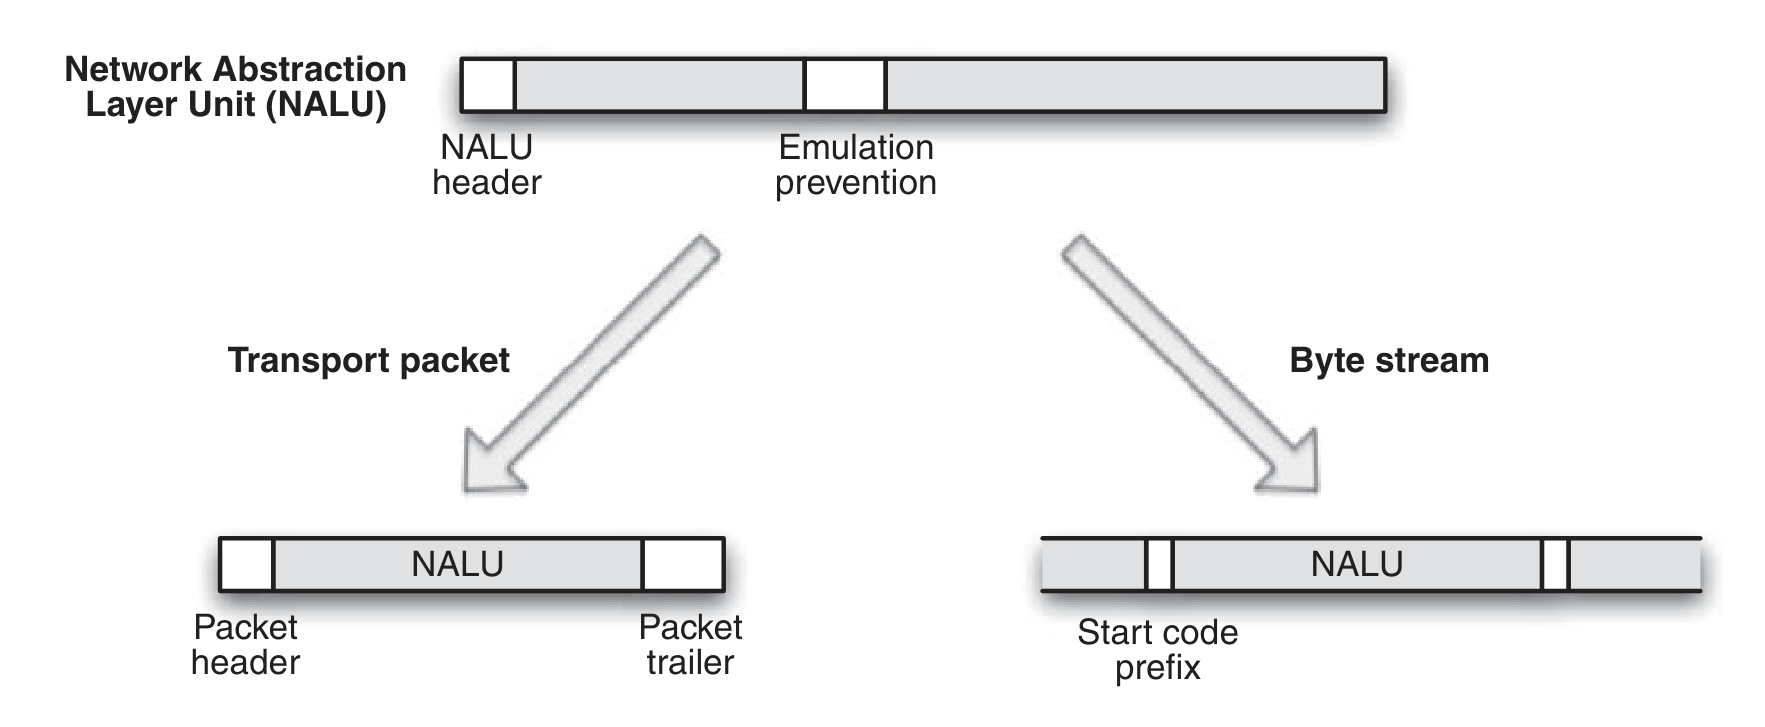
\includegraphics[width=0.9\textwidth]{res/h264_nalu.png}
	
	\caption{H.264 bitstream structure and encapsulation alternatives.}
	\label{fig:h264_encapsulation}
\end{figure}

\section{Digital audio and compression}
\label{sec:bg/audio}

Digital audio is generally represented through the \textbf{Pulse Code Modulation} (PCM) method, which is characterized by two main parameters: \textbf{sample rate}, which defines how frequently the sound level was measured when captured from the analog domain, and \textbf{bit depth}, which refers to the number of bits used to store a sample.

Although uncompressed PCM audio is more tractable than video, since it is much lighter (a stereo audio track with 44.1 kHz sample rate and 16-bit samples requires "only" 1.4 Mbps), audio is typically highly compressible since human sound perception is limited. Audio coding formats such as \textbf{MP3} and \textbf{AAC} are based on perceptual coding, as they tend to discard sound information that would otherwise be inaudible and can achieve excellent quality with savings of up to 90\%.\cite{aac}

\textbf{AAC} is nowadays the most widely used audio format in streaming scenarios and is supported by virtually every device.\cite{bitmovin} AAC comes in multiple variants, with \textbf{Low Complexity} (AAC-LC) being the most common, since it is widely supported and provides good compression ratios and quality. Other common versions are the ones of the \textbf{High Efficiency} (HE) family, which are optimized for low-bitrate applications.

In the AAC bitstream, audio samples are organized into packets that contain a fixed number of samples, typically 1024. To reduce compression artifacts, AAC uses a modified version of the DCT transform that works with overlapping samples. This means that in practice, for each AAC packet encoded or decoded another packet with the same number of samples is required. For this reason, AAC encoders add at least 1024 samples of silence before the first actual audio sample, a technique called \textbf{priming}. Since this delay could introduce synchronization issues when audio is combined with video, decoders need to detect priming and correctly take into account the encoder delay.\cite{aacpriming}

\section{Container formats}
\label{sec:bg/containers}

Bitstreams produced by video and audio encoders often do not contain enough information to allow video players to actually play the video or audio file. For example, in H.264 the timing information is optional and without it the decoder does not know how to assign timestamps to individual video frames, or even determine the duration of the video.\cite{h264itu} In AAC, the raw frames do not contain information like the sample rate or even the variant of AAC used to encode the samples.\cite{aac}

\textbf{Container formats} solve this problem by wrapping the bitstreams in a structure that is common between different coding formats. Container formats also allow the grouping of multiple video, audio and subtitle tracks, an operation known as \textbf{muxing} (from \textit{multiplexing}) and performed by \textbf{muxers}. The process of extracting tracks from a container format is instead known as \textbf{demuxing}.

Two popular container formats used in the context of video streaming are \textbf{MPEG-2 Transport Stream} and \textbf{MP4}.

\subsection{MPEG-2 Transport Stream}
\label{sec:bg/containers/mpeg2ts}

MPEG-2 Transport Stream (or \textbf{MPEG-2 TS}), defined by the MPEG-2 Part 1 standard, is a container format originally designed for digital television broadcasting systems. For this reason, it includes features such as error correction and synchronization, providing protection against degraded transmission channels.

A single MPEG-2 Transport Stream can transport multiple programs, for example multiple TV channels. Each program can consist of multiple video and audio streams, known as \textbf{elementary streams}. The coded data for each elementary stream is packetized into PES (Packetized Elementary Stream) packets, each having a fixed length of 188 bytes. The 188 bytes include headers (which transport data like timing information), which is the reason why Transport Stream often has a non-negligible overhead.\cite{mpeg2ts}

% terrible, rewrite
% https://tsduck.io/download/docs/mpegts-introduction.pdf

An H.264 bitstream muxed in an MPEG-2 stream must be in the Annex B format with start codes.

\subsection{MP4 and fragmented MP4}
\label{sec:bg/containers/mp4}

MP4 is a container file format based on the \textbf{ISO Base Media File Format} (ISOBMFF). It was extended from Apple's QuickTime File Format (\texttt{.mov}) and first published in 2001 as MPEG-4 Part 14.\footnote{The actual box structure is defined in MPEG-4 Part 12 (ISOBMFF).}\cite{mpeg4part12}

In the \textbf{ISOBMFF} format, the video and audio bitstreams, such as an H.264-compressed video, are stored as tracks and organized in a \textbf{box structure}. The MP4 format is capable of storing metadata like the video duration and per-frame display and decoding timestamps, dealing with issues like synchronization between tracks and random access (\textit{seeking}) of the media file.

% Video and audio frames are usually interleaved, although it is possible to generate "flat" MP4 files where tracks are organized sequentially.

Some ISOBMFF box (or atom) types that are particularly relevant are:

\begin{itemize}
    \item \texttt{ftyp} (\textit{file type}), which includes some general information about the file type, e.g. the version of the MP4 (or QuickTime) specification the file is compliant against.
    \item \texttt{moov} (\textit{movie header}), containing metadata about the tracks, such as the creation time, the duration, the resolution, bitrate, the tables that allow players to quickly find the part of the file where a specific frame or timestamp can be found, etc.
    \item \texttt{mdat} (\textit{movie data}), containing the actual audio and video samples.
\end{itemize}

An H.264 bitstream muxed in an MP4 container does not need start codes and therefore must not be in the Annex B format. H.264 bistreams in MP4 files are stored in a format known as \texttt{avcC}, where H.264 NAL units are prepended with their length.

A typical structure of an MP4 file consists of a \texttt{ftyp} box followed by a \texttt{moov} box (containing the tracks metadata), and finally the actual data stored in a \texttt{mdat} box. The \texttt{moov} box is sometimes placed at the end of the file, since the information required to create the box is often available only at the end of the encoding process.

% TODO: mp4dump example

For some use cases, like adaptive video streaming, a more suitable structure is the one provided by the \textbf{fragmented MP4} format, or \textbf{fMP4}. In this format, the sequence is divided in fragments that can be transmitted and played independently. The structure of a fMP4 file still has \texttt{ftyp} and \texttt{moov} boxes at the beginning, shared among all the fragments, while the rest of the file consists of a sequence of \texttt{moof} and \texttt{mdat} boxes, where the \texttt{moof} box contains metadata about the fragment, like the fragment index and the timestamp, and the \texttt{mdat} contains the video or audio samples for a single fragment (typically a few seconds of content).

% TODO: mp4dump example

\section{A typical live streaming architecture}
\label{sec:bg/architecture}

In a live streaming architecture, we can generally distinguish three main parts: \textbf{ingestion}, \textbf{transcoding and packaging}, and \textbf{distribution}.

\textbf{Ingestion} refers to the process of making the input feed available to the transcoder server for processing. Often, this means having a client push the stream through an ingestion protocol such as \textbf{Real Time Messaging Protocol} (RTMP). In some cases, a more suitable approach is a pull-based one, where it is the backend system's responsibility to "pull" the video and audio streams from another system and pass them onto the pipeline.

Usually, the input feed is a high-bitrate/high-quality stream that is not suitable for live streaming. In particular, when the setup is based on adaptive bitrate streaming (ABR), which is the de facto standard for live streaming, the video stream must be \textbf{transcoded} in multiple video renditions with different quality levels and encoding parameters. The video and audio files produced by this step need to be in a coding and container format that is compatible with the adaptive bitrate technology that was chosen. For example, MPEG-DASH (see Section \ref{sec:bg/technologies/dash}) requires streams to be muxed in a fragmented MP4 container.

Ideally, for the best performance, the video files produced in this step should take into account how ABR technologies work. For example, the bitrate of the individual renditions should not oscillate too much so that bitrate adaption algorithms can take the average bitrate as a reference value. Also, since segments should be roughly of the same size a fixed GOP size should be used when encoding.\cite{ozer}

Additionally, some adaptive streaming technologies require the video fragments (or segments) to be stored in physically separated files. The task of splitting video and audio files into smaller segments is done by \textbf{packagers}, which can be static or dynamic: with \textbf{static packaging} the individual video fragment files are actually created and stored on disk, while with \textbf{dynamic packaging} they are generated on the fly. The packager, which is specific for the ABR technology, also creates \textbf{manifest or playlist files} that act as an index for the streams.

The segmented video and audio tracks, together with the manifest files, can finally be delivered to clients. Most of the time, this is done through the Hypertext Transfer Protocol (HTTP). Using HTTP makes it easy for streaming platforms to scale, thanks to the widespread availability of \textbf{Content Delivery Networks} (CDN) and their global distribution networks. One of the important advantages of relying on CDNs is the possibility to cache video segments at the edge of the networks, as close as possible to the final users, therefore reducing latency and probability of congestion.

% architecture diagram

% TODO: probably merge this section with the below one and be more precise with terminology. See NMD report.

% TODO: packager or segmenter

% advantages of HTTP: no UDP, firewalls, scalability, https

\section{Adaptive bitrate technologies}
\label{sec:bg/abr}

\subsection{Apple HTTP Live Streaming (HLS)}
\label{sec:bg/abr/hls}

HTTP Live Streaming (HLS) is an HTTP-based adaptive streaming protocol designed by Apple. First introduced in 2009 and later standardized as RFC 9216, it is estimated to be the most popular streaming protocol with more than 73\% companies using it.\cite{rfc8216}\cite{bitmovin} The reason for that is not only the fact that HLS is the only possible option to implement live and on demand streaming on Apple mobile devices and browsers, but also the simplicity of the protocol.

HLS uses the \textbf{extended M3U format} (\texttt{.m3u8} extension) to define a set of playlists that contain information such as the list of streams or the list of segments for a particular stream. In particular, a \textbf{master playlist} provides a set of variant streams\footnote{In the HLS RFC, the terms \textit{variant} and \textit{rendition} have different meanings. We will use the term \textit{variant} in this section to adhere to the RFC, while using the two terms interchangeably in the rest of the thesis.}, each of which is a different version of the same content, usually differing by bitrate and other encoding parameters. Players download the master playlist at the beginning of the playback session and use the information contained in it to adapt to network conditions by switching between variants. An example of a master playlist is shown in Figure \ref{fig:hls_master}.

\begin{figure}[h]
    \centering
    \begin{minted}[frame=single]{text}
#EXTM3U
#EXT-X-STREAM-INF:BANDWIDTH=1280000,AVERAGE-BANDWIDTH=1000000
low.m3u8
#EXT-X-STREAM-INF:BANDWIDTH=2560000,AVERAGE-BANDWIDTH=2000000
mid.m3u8
#EXT-X-STREAM-INF:BANDWIDTH=7680000,AVERAGE-BANDWIDTH=6000000
high.m3u8
#EXT-X-STREAM-INF:BANDWIDTH=65000,CODECS="mp4a.40.5"
audio-only.m3u8
    \end{minted}
	\caption{Example of a HLS master playlist with variants. The first three variants contain both video and audio, while the fourth variant is audio-only. The first variant, corresponding to the \texttt{low.m3u8} media playlist, is defined with an average bitrate of 1000 kbps and a peak bitrate of 1280 kbps.}
	\label{fig:hls_master}
\end{figure}

When players want to play a specific variant, they load the \textbf{media playlist} corresponding to the variant. A media playlist must specify the maximum duration of segments in seconds, followed by a list of \textbf{media segments}, characterized by their duration and URI (relative or absolute). In the case of on-demand content, the media playlist must contain the full list of segments that make up the video or audio file, while in the case of live streams, the playlist may include only a sliding window of segments. An example of a media playlist is shown in Figure \ref{fig:hls_media}.

\begin{figure}[h]
    \centering
    \begin{minted}[frame=single]{text}
#EXTM3U
#EXT-X-TARGETDURATION:6
#EXT-X-VERSION:3
#EXTINF:6,
segment-1.ts
#EXTINF:6,
segment-2.ts
#EXTINF:3,
segment-3.ts
#EXT-X-ENDLIST
    \end{minted}
	\caption{Example of a simple HLS VOD media playlist with three segments and a segment target duration of 6 seconds.}
	\label{fig:hls_media}
\end{figure}

HLS media segments can be muxed in MPEG-2 TS format (\texttt{.ts} files) or fragmented MP4 format (\texttt{.mp4} or \texttt{.m4s} files), while supported video codecs are H.264 and H.265. When using \texttt{fMP4} as a container format, media playlists must specify an \textbf{initialization segment} containing the \texttt{ftyp} and \texttt{moov} boxes through the \texttt{\#EXT-X-MAP} tag.

In addition to the RFC, Apple maintains an \textit{Authoring Specification for Apple Devices} defining additional rules for HLS streams, which are often taken as best practices in the industry when producing content for adaptive bitrate streaming.\cite{hlsauthoring}

The authoring specification provides a set of recommendations to ensure compatibility with HLS implementation that can be found on Apple devices, including:

\begin{itemize}
    \item a table with a possible set of variants with their bitrate and frame rate (a \textit{bitrate ladder}), for both H.264 and H.265, plus a recommendation to adjust them according to the specific use case;
    \item an indication that the peak bitrate should be no more than 200\% of the average bitrate, although it is often recommended to make the bitrate as constant as possible;\cite{ozer}
    \item a recommendation for a segment duration of 6 seconds, although 4 seconds or lower are common values in practice.\cite{ozer}
\end{itemize}

HLS also includes support for encryption, ads, trick play (scrubbing and fast forward), subtitles, and multiple audio tracks.

% TODO: low-latency HLS

\subsection{MPEG Dynamic Adaptive Streaming over HTTP (DASH)}
\label{sec:bg/technologies/dash}

% TODO

\subsection{Common Media Application Format (CMAF)}
\label{sec:bg/technologies/cmaf}

Before Apple introduced support for \texttt{fMP4} in 2016, a common issue for video platforms was that supporting both HLS and DASH required two copies of the same content, one in MPEG-2 TS format and the other in \texttt{fMP4}.

This led to the proposal and standardization of \textbf{Common Media Application Format} (CMAF), a common specification that defines how media should be packaged and segmented for delivery. Fragmented MP4 is a CMAF-compatible format and since it is supported by both HLS and DASH it can lead to significant savings. Video platforms can, in fact, produce and store a single set of video segment files that can be delivered to all devices.\cite{cmaf}

\subsection{Media Source Extensions (MSE)}
\label{sec:bg/technologies/mse}

One of the main medium through which users watch video streams is web browsers. Apple includes native support for its HLS protocol in Safari, which is preinstalled on all Apple devices and is also the only engine that can be used on iOS. Other browsers typically do not include support for HLS and DASH, but instead support the \textbf{Media Source Extensions} (MSE) API, through which JavaScript libraries can implement HLS and DASH.\cite{mse}

MSE is a set of APIs that abstract the implementation of media playback in the browser. MSE exposes types and methods that allow the client-side code to push video and audio data for playback.

More in detail, MSE defines the \texttt{MediaSource} type as a source of media data for the \texttt{<video>} or \texttt{<audio>} HTML5 media elements, to which a \texttt{MediaSource} is attached. The client code interacts with the \texttt{MediaSource} to push new data, while the media elements fetch the data from the \texttt{MediaSource}.

\texttt{MediaSource} instances expose methods to attach a set of \texttt{SourceBuffer} objects, which represent individual media tracks like a video or audio streams. When new media data is available, such as a new video segments, the client calls the \texttt{appendBuffer()} method on the corresponding \texttt{SourceBuffer}, providing the new data for the track to the browser. The bytes of data must of course conform to the format set when creating the \texttt{SourceBuffer}, which must be supported by the browser. Most of the time this means ISOBMFF (\texttt{fMP4}) or WebM as container formats, while codecs often depend on the browser build and platform.

Libraries that implement HLS or DASH must take care of parsing the manifest files, downloading the segments, implementing rate adaption algorithms, potentially transmuxing from MPEG-2 TS to fragmented MP4 (such as with HLS), appending segment data to the source buffers while leaving the MP4 demuxing and stream decoding tasks to the browser.

In practice, this means that there can be many implementations of HLS and DASH, all relying on Media Source Extensions underneath. For HLS, a popular implementation is \texttt{HLS.js}\footnote{\url{https://github.com/video-dev/hls.js/}}, while for DASH the official reference implementation is \texttt{dash.js}\footnote{\url{https://github.com/Dash-Industry-Forum/dash.js/}}. Several other JavaScript players include support for HLS and DASH, such as \texttt{Video.js}, \texttt{Shaka Player}, \texttt{THEOPlayer}, and \texttt{JW Player}, some of which are open source while others are commercial.

\section{Hypertext Transfer Protocol (HTTP) evolution}
\label{sec:bg/http}

When browsing the Web, we use an application layer protocol known as \textbf{Hypertext Transfer Protocol} or \textbf{HTTP}. In addition to being used for transferring HTML web pages and related files, we have seen that HTTP can be used by apdative streaming technologies to deliver video and audio segments to the client.

In this section, we will briefly go through three important versions of HTTP, their limitations, peculiarities, and how they are currently exploited by HLS and DASH for video streaming applications.

% TODO: mention LL-HLS and LL-DASH somewhere?

\subsection{HTTP/1.1}
\label{sec:bg/http1}

For a long time, the dominant HTTP version has been HTTP/1.1, first published in 1997.\cite{http1.1} It is based on the Transmission Control Protocol (TCP), the reliable connection-oriented transport layer protocol.

To send an HTTP request, a client should open a TCP connection with the server. It will then transmit the request line, followed by a list of headers, an empty line, and optionally a payload or message body. The following is an example of an HTTP/1.1 \texttt{GET} request to the URL \texttt{http://example.com/index.html}.

\begin{minted}[frame=single]{http}
GET /index.html HTTP/1.1
Host: example.com
User-Agent: curl
Accept: */*
\end{minted}

Once the server has received the request, it will do its processing and then start sending the response on the same TCP connection. The response consists of a status line, a list of headers, and optionally a message body, as in the following example.

\begin{minted}[frame=single]{http}
HTTP/1.1 200 OK
Date: Thu, 22 Dec 2022 08:00:00 GMT
Content-Type: text/html; charset=UTF-8

<html>
<head>
...omitted...
\end{minted}

For encrypted communication, HTTPS uses \textbf{Transport Layer Security} (TLS) to create a secure communication channel over TCP. The HTTP/1.1 request is then transmitted on top of the encrypted TLS session.

When keep-alive is enabled (persistent connections), the same connection can be reused to send multiple HTTP requests, avoiding the overhead of establishing a new TCP connection and TLS session. HTTP/1.1 also supports request pipelining, meaning that multiple requests can be sent on the same TCP connection before receiving the responses, although it is rarely used because not all server implementations support it properly.

The main limitation of HTTP/1.1 is, however, that it does not support responses multiplexing, meaning that responses must be transmitted sequentially. This causes a problem known as \textbf{HTTP head-of-line blocking}, where the current request blocks the following requests. Browsers try to workaround this issue by opening multiple TCP connections to the same web server when loading web pages, up to a (configurable) limit.\footnote{For example, Firefox uses 6 as a default connection limit, but the value can be changed through the \texttt{network.http.max-persistent-connections-per-server} preference.} 

\subsection{HTTP/2}
\label{sec:bg/http2}

HTTP/2, published as a Proposed Standard in 2015 as RFC 7540, was an attempt to solve the main issues of HTTP/1.1, most notably the head-of-line blocking problem. The aim of HTTP/2 was at the same time to use less network resources while reducing the perception of latency.\cite{http2}

In HTTP/2, clients establish a \textbf{single TCP connection} with the server. To allow request and response \textbf{multiplexing}, the protocol introduces a binary framing format in which requests and responses, which maintain the same HTTP semantics as in HTTP/1.1, are split into smaller units, the frames. Frames can be interleaved, allowing multiple requests and responses to be transmitted in parallel. In order to identify to which request a frame belongs to, the concept of \textbf{streams} was introduced. Streams can be seen as virtual connections that are very light to create and generally correspond to single HTTP requests. Streams can also be reset, with the effect of immediately stopping the transmission of data frames.

An important feature of HTTP/2 is \textbf{stream prioritization}. Since multiple streams can co-exist on the same TCP connection, there was the need for a mechanism to make better decisions on which stream goes first or is given priority. HTTP/2 allows clients to assign a \textbf{weight} between 1 and 256 to each stream, where a higher number means higher priority. In addition, clients can specify that a stream is dependent on another stream through its ID, effectively creating a \textbf{dependency tree}. The structure of the tree, and therefore the order in which requests are responded, is defined by the dependency relationships, while the division of resources between a set of "children" streams is determined by their weights.

The dependency tree approach of HTTP/2 is very flexible and allows clients to implement different \textbf{prioritization strategies}, with widely different performance results. In \cite{http2pri}, Wijnants et al. examined the behavior of the main browsers to find out which prioritization scheme they implemented. It turns out that only Mozilla Firefox chose to adopt a complex tree-based strategy. Google Chrome implements a much simpler sequential FCFS approach based on dynamic weights (giving more weight to more requests deemed more important according to heuristics), Microsoft Edge (legacy) uses a naive round-robin strategy with no weights at all, while Safari follows a weighted round-robin scheme. Surprisingly, experimental results showed superior performance when the simple strategy implemented by Chrome is used.

% TODO: diagrams
% https://speeder.edm.uhasselt.be/www18/files/h2priorities_mwijnants_www2018.pdf
% https://speeder.edm.uhasselt.be/www18/files/h2priorities_mwijnants_www2018_presentation.pdf
% https://speeder.edm.uhasselt.be/www18/
% https://quic.edm.uhasselt.be/files/fosdem.pdf
% https://youtu.be/nH4iRpFnf1c?t=440

In HTTP/2, the use of HTTPS is mandatory, making the protocol more secure by design. HTTP/2 also achieves better performance by compressing headers, thanks to the \texttt{HPACK} compression algorithm. Finally, a feature known as \textbf{HTTP/2 Server Push} allows the server to push additional unsolicited content in response to HTTP requests, theoretically reducing the need of additional round-trip times to request resources.

While all these features make sense, in practice HTTP/2 did not manage to provide the expected performance improvements, for multiple reasons:

\begin{itemize}
    \item The Server Push feature never really took off, with virtually no CDN having support for Server Push. Additionally, in 2022 Google removed Server Push support from Google Chrome citing extremely low usage, almost no gain in performance, and complexities in browser implementation, suggeting developers to instead use the preload hints or \textbf{103 Early Hints} features.\footnote{\url{https://developer.chrome.com/blog/removing-push/}}
    \item Stream prioritization was found to be inconsistently implemented by clients and servers, with a significant number of large CDNs apparently ignoring prioritization.\footnote{\url{https://github.com/andydavies/http2-prioritization-issues}}. This led to the prioritization scheme of HTTP/2 being deprecated and replaced by a new mechanism at the same time that HTTP/3 came out.
    \item The sequential prioritization strategy leads to the same HTTP head-of-line blocking issue seen in HTTP/1.1, worsened by the fact that only a single TCP connection is used.
    \item The use of a single TCP connection leads to another problem known as \textbf{TCP head-of-line blocking}, where the bottleneck is not the HTTP design but TCP itself. In fact, while HTTP/2 multiplexes requests in multiple streams, at the transport layer TCP only sees a single opaque byte stream. As a consequence, TCP retransmissions delay the transmission of all streams and not just the one affected by packet loss. Additionally, TCP congestion control may reduce the throughput of the connection in case of congestion, affecting all the requests, while in HTTP/1.1 it is less likely that all the connections are affected at the same time.
\end{itemize}

\subsection{HTTP/3}
\label{sec:bg/http3}

To overcome the limitations of TCP-based approaches, HTTP/3 is based on a new transport protocol called QUIC, which is built on top of the lightweight UDP. While HTTP/3 by itself does not introduce new features, the fact that it is based on a new protocol like QUIC allowed to rethink how a transport layer protocol should work from the ground up. QUIC was published as a Proposed Standard with RFC 9000 in May 2021 with HTTP/3 following as RFC 9114 in June 2022, after a few years of work.\cite{http3}

In particular, these are the main difference between HTTP/2 and HTTP/3 based stacks:

\begin{itemize}
    \item Since QUIC is based on UDP, TCP features such as connection establishment, flow control, congestion control, and retransmissions are now implemented by QUIC;
    \item \textbf{TLS v1.3} is tightly integrated with QUIC, making security features like encrypted communication mandatory while allowing innovative features like 1-RTT handshakes or 0-RTT session resumption to be implemented seamlessly, further improving performance;
    \item Unlike TCP, QUIC provides a seamless \textbf{connection migration} feature that allows reuse of connections when network connection changes;
    \item \textbf{Stream multiplexing} is moved "down" from the application layer to QUIC. HTTP/3 takes advantage of QUIC streams to provide request multiplexing. HTTP/3 clients or servers can cancel HTTP requests by \textbf{resetting} the underlying QUIC stream;
    \item HTTP/2 \textbf{stream prioritization} is replaced by a simpler priority mechanism, implemented at the HTTP/3 level. QUIC does not have stream prioritization.
\end{itemize}

% TODO: stack diagrams https://github.com/rmarx/h3-protocol-stack/blob/main/README.md

The \textbf{head-of-line blocking} issue caused by TCP in HTTP/2 is not present in HTTP/3 because streams are now a concept of the transport layer. Unlike TCP, in fact, QUIC does not see a single byte stream but multiple streams that can be treated independently (with respect to retransmissions, for example). However, if the scheduling strategy implemented by the server is sequential, there could still be head-of-line blocking because the slow transmission of a stream would block the other ones. The multiplexing scheduler depends on the server implementation and is often round-robin, according to the experiments run by Marx et al.\cite{quicdiversity}

The prioritization scheme used by HTTP/3 was introduced in RFC 9218, published together with HTTP/3, with the title of \textit{Extensible Prioritization Scheme for HTTP}. As the title suggests, the new mechanism is actually not HTTP/3-specific and is defined for both HTTP/2 and HTTP/3. Clients that implement RFC 9218 can communicate their preferences on how the server should prioritize responses in two ways:\cite{rfc9218}

\begin{itemize}
    \item Through an HTTP header called \texttt{Priority}, where the priority for the request is specified.
    \item Through a \texttt{PRIORITY\_UPDATE} frame, that makes it possible to reprioritize requests after they have been sent. With HTTP/3, priority update frames are transmitted over a unidirectional QUIC stream dedicated to control commands.
\end{itemize}

Requests priorities in RFC 9218 are defined by two parameters:

\begin{itemize}
    \item the \textbf{urgency} parameter (\texttt{u}), an integer value ranging from 0 to 7 in descending order of priority, with a default value of 3;
    \item the \textbf{incremental} parameter (\texttt{i}), indicating whether an HTTP response can be processed incrementally by the client, and therefore if it can benefit from being received concurrently. For example, the download of a standard JPEG image file would not benefit from being transmitted incrementally since the JPEG decoder usually needs the whole image to start decoding the picture. On the other hand, a CSS file could benefit from being delivered even partially if the browser is capable of interpreting the CSS rules before the whole file is downloaded. The default value for the incremental parameter is 0 (\texttt{false}).
\end{itemize}

When using the \texttt{Priority} header, the urgency and incremental parameters can be specified as a string in the following format: \texttt{u=3, i=0}.

Since HTTP/3 uses the same transport layer port as previous HTTP versions, namely port 443 for HTTPS, but with a different transport layer protocol (TCP vs QUIC), a protocol negotiation mechanism is needed. This is done through the HTTP \texttt{Alt-Svc} response header, through which servers can specify if and on which port alternative services such as HTTP/3 are available. Browsers usually send the first connection through TCP-based HTTP. If the response contains an \texttt{Alt-Svc} header indicating that HTTP/3 is available, they close the TCP connection and switch to QUIC on subsequent requests. An example of a header advertising HTTP/3 on port 443 is \verb|Alt-Svc: h3=":443"; ma=2592000|, where \texttt{ma} (max-age) corresponds to the number of seconds for which the alternative service configuration should be considered valid (defaults to 24 hours).

\subsubsection{Server implementations}
\label{sec:bg/http3/servers}

Even before the QUIC specification was published, several open-source libraries that implement QUIC were born. Some of the most notable ones are Cloudflare's \texttt{quiche}, Fastly's \texttt{quicly}, Google's \texttt{quiche}, Meta's \texttt{mvfst}, and LiteSpeed's \texttt{lsquic}.\cite{quicdiversity}

Some of these libraries also provide support for HTTP/3, although they are not HTTP web servers that can be used out of the box. Popular web servers like \textbf{Apache} and \textbf{nginx} do not currently support HTTP/3. Specifically, nginx support for HTTP/3 was delayed because OpenSSL, the TLS implementation used by nginx, still has to implement the required interfaces for QUIC. nginx is therefore planning to switch to another TLS library and expects HTTP/3 support to be finalized by the end of 2022.\footnote{\url{https://www.nginx.com/blog/our-roadmap-quic-http-3-support-nginx/}}

Some lesser known web servers that include HTTP/3 support are Fastly's h2o (based on \texttt{quicly}), LiteSpeed Web Server (based on \texttt{lsquic}), and Caddy (based on \texttt{quic-go}).

\subsubsection{Browser support}
\label{sec:bg/http3/browsers}

It is estimated that around 75\% of the market share of browsers is capable of browsing with HTTP/3. Google Chrome added support for HTTP/3 in 2020, Mozilla Firefox in 2021, while Apple's Safari still considers HTTP/3 support experimental at the time of writing.\footnote{\url{https://caniuse.com/http3}} According to Cloudflare Radar, HTTP/3 traffic accounts for around 28\% of global web traffic, with HTTP/2 at 65\% and HTTP/1.x at 7\%.\footnote{\url{https://radar.cloudflare.com/}}

\subsubsection{Debugging tools}
\label{sec:bg/http3/tools}

When conducting research or developing applications that use HTTP/3 features, it is often useful to dig deeper into the raw HTTP/3 or QUIC frames. There are several tools that make this possible:

\begin{itemize}
    \item \textbf{Wireshark}, the popular network protocol analyzer, which includes support for QUIC and HTTP/3, although still very basic and missing most features;\footnote{\url{https://gitlab.com/wireshark/wireshark/-/issues/16761}}
    \item \texttt{qlog}, a project by the IETF QUIC Working Group aimed at introducing a common logging format for QUIC. Both client and server implementations can support \texttt{qlog}, providing a way to capture and export network traces with QUIC-related events in a common format. \texttt{qlog} captures could then be parsed by \texttt{qlog} analyzers;\footnote{\url{https://github.com/quicwg/qlog}}
    \item Chrome's \textbf{NetLog dump}, a detailed capture of network activity from the perspective of the browser. It can be generated by browsing to \texttt{chrome://net-export}. The format is proprietary, but there are visualization tools that support the NetLog format;\footnote{\url{https://www.chromium.org/for-testers/providing-network-details/}}
    \item \texttt{qvis}, developed by the authors of \cite{quicdiversity}, a suite of tools that analyze \texttt{qlog}, NetLog dumps or Wireshark captures to provide advanced insights into QUIC traces. The suite includes many visualization tools such as sequence diagrams, congestion control plots, multiplexing and packetization visualizations, and other detailed statistics.\footnote{\url{https://qvis.quictools.info/}}
\end{itemize}

\section{Network emulation}
\label{sec:bg/network}

When developing network-based applications or running benchmarks against the network, it is often useful to be able to setup a testbed that emulates an actual network. There are several software tools that do that, among which there are \textbf{Mininet} and \textbf{ComNetsEmu}, which we will briefly explain in the following sections.

\subsection{Mininet}
\label{sec:bg/network/mininet}

\textbf{Mininet} is an emulation tool that allows to create realistic virtual networks on a single machine. In Mininet you can create hosts and switches, connect them through links and make them interact. It also supports \textbf{Software-Defined Networking}, making it possible to have switches controlled by an SDN controller through the OpenFlow protocol.

With Mininet you can create arbitrarily complex custom topologies through the CLI or the Python API, all on a single machine thanks to its light impact. Unlike traditional virtualization-based approaches, Mininet implements lightweight OS-level network virtualization by using features of the Linux kernel, such as network namespaces. The result is that Mininet boots much faster, usually in seconds, can easily scale with modest system requirements and performs well with high-bandwidth applications.\footnote{\url{http://mininet.org/overview/}}

\begin{figure}
    \centering
    \begin{minted}[frame=single,linenos,highlightlines={18,22,28,36,42},fontsize=\small]{bash}
$ sudo mn
*** Creating network
*** Adding controller
*** Adding hosts:
h1 h2
*** Adding switches:
s1
*** Adding links:
(h1, s1) (h2, s1)
*** Configuring hosts
h1 h2
*** Starting controller
c0
*** Starting 1 switches
s1 ...
*** Starting CLI:

mininet> nodes
available nodes are:
c0 h1 h2 s1

mininet> net
h1 h1-eth0:s1-eth1
h2 h2-eth0:s1-eth2
s1 lo:  s1-eth1:h1-eth0 s1-eth2:h2-eth0
c0

mininet> h1 ping -c 1 h2
PING 10.0.0.2 (10.0.0.2) 56(84) bytes of data.
64 bytes from 10.0.0.2: icmp_seq=1 ttl=64 time=2.51 ms

--- 10.0.0.2 ping statistics ---
1 packets transmitted, 1 received, 0% packet loss, time 0ms
rtt min/avg/max/mdev = 2.507/2.507/2.507/0.000 ms

mininet> pingall
*** Ping: testing ping reachability
h1 -> h2
h2 -> h1
*** Results: 0% dropped (2/2 received)

mininet> iperf
*** Iperf: testing TCP bandwidth between h1 and h2
.*** Results: ['21.0 Gbits/sec', '21.0 Gbits/sec']
    \end{minted}
    \caption{Example of usage of the Mininet CLI with the default \texttt{minimal} topology. Mininet allows to run Linux network tools such as ping and iperf directly on the virtual hosts.}
    \label{fig:mininet}
\end{figure}

\subsection{ComNetsEmu}
\label{sec:bg/network/comnetsemu}

\textbf{ComNetsEmu} is an extension to Mininet that aims at complete host isolation thanks to \textbf{Docker containers}. Since ComNetsEmu enforces stricter node isolation, it is heavier than Mininet.

Similarly to Mininet, ComNetsEmu can be programmed through the Python API. Hosts are Docker containers and applications deployed on hosts are Docker containers too. The application containers are deployed as siblings containers to emulate a "Docker-in-Docker" behavior.

The recommended way to run ComNetsEmu is to use a Vagrant virtual machine, which takes care of setting up the software and all the required dependencies.\cite{comnetsemu}

% TODO: maybe network patterns

      \chapter{Quality of experience evaluation}
\label{cha:eval}

In this section, we will illustrate how we set up a \textbf{testbed} with ComNetsEmu to evaluate the performance of \textbf{low-latency adaptive bitrate live streaming}. We will then present some of the results that we obtained. In fact, the testbed allows to extract and plot some important metrics, which will highlight some of the issues of current streaming technologies in low-latency scenarios.

The results of the evaluation will be the basis for the improvements proposed in Section X. We believe that these improvements produce a better overall \textbf{quality of experience} for a live stream.


\section{Testbed setup}
\label{sec:eval/testbed}

The testbed for evaluating the quality of experience (QoE) of live streaming solutions was built with ComNetsEmu. The project was published as an open source project at \url{https://github.com/matteocontrini/live-streaming-testbed}.

The general architecture of the testbed is shown in Figure X. The topology of the emulated network consists of three hosts (H1, H2, H3) and two switches (S1, S2). The link between the two switches represents an unreliable network such as an Internet access network. When the emulation is run, a series of experiments with different configurations are run, and the link parameters are changed. For example, the bandwidth is varied to emulate a real network with oscillating throughput.

On the three hosts, several applications are deployed as Docker containers.

\begin{itemize}
    \item \texttt{H3} hosts a script that performs the \textbf{packaging of a live stream} in both HLS and DASH formats. It runs an \ffmpeg{} command that simulates a live stream, taking an MP4 file as input. The output of this application, called \textit{live source}, are manifest and playlist files for both HLS and DASH and the corresponding video and audio segments in \texttt{fMP4} format.
    \item \texttt{H2} acts as an \textbf{HTTP CDN server} for the packaged stream. In practice, it is an \texttt{h2o} web server that serves the files produced by the live source, over HTTP/1.1, HTTP/2 and HTTP/3. It also takes care of provisioning the public key certificates that are required for HTTPS.
    \item \texttt{H1}, which is on the other side of the main network link, is the client. It consists of a frontend application containing a \textbf{video player} that plays the live video stream generated by the server. The frontend application also takes care of collecting several metrics from the player and transmitting them to a Node.js backend application. The frontend application runs in a \textbf{Chromium headless} instance, which is started by the backend application through the \textbf{Puppeteer} library.
\end{itemize}

% TODO: diagram

To start the emulation through ComNetsEmu, one first needs to clone the source code of the testbed. The ABR video renditions should then be encoded and written in an MP4 file, which the live source will then use to simulate the live stream (we will see this in detail in Section \ref{sec:eval/testbed/packaging}). To start the Vagrant virtual machine and start a session, the following commands can be used.

\begin{minted}[frame=single]{bash}
vagrant up
vagrant ssh
\end{minted}

Finally, after building the Docker images, the emulation can be started, as shown in the following code block. The testbed source code actually contains scripts that can be used to execute these commands more easily. They also handle error handling and cleanup.

\begin{minted}[frame=single]{bash}
cd live-source && docker build -t live-source .
cd ../cdn && docker build -t cdn .
cd ../client && docker build -t client .
cd .. && sudo python3 topology.py
\end{minted}

Before going into the details of how the specific components were developed, it should be noted that the default Vagrant configuration for ComNetsEmu (contained in a file known as \texttt{Vagrantfile}) does not work when the machine architecture is ARM. This is especially problematic on newer laptops that use Apple Silicon hardware, such as the M1 and M2 chips.

To solve this problem, two changes must be applied to the ComNetsEmu \texttt{Vagrantfile}. First, the Vagrant box (the operating system image) must be changed to an image that is built for the ARM architecture. Then, since x86 virtualization software such as VirtualBox cannot be used on ARM systems, a new virtual machine provider must be added. In practice, for Mac systems, this means enabling Parallels Desktop as a virtual machine provider. Figure \ref{fig:vagrantfile} shows how the \texttt{Vagrantfile} of ComNetsEmu was modified for Apple Silicon support.

\begin{figure}
    \centering
    \begin{minted}[frame=single,linenos,fontsize=\small]{diff}
diff --git a/Vagrantfile b/Vagrantfile
index 0f07076..a21824f 100644
--- a/Vagrantfile
+++ b/Vagrantfile
@@ -20,6 +20,8 @@ VM_NAME = "ubuntu-20.04-comnetsemu"
 # When using libvirt as the provider, use this box, bento boxes do not support...
 BOX_LIBVIRT = "generic/ubuntu2004"

+BOX_PARALLELS = "jeffnoxon/ubuntu-20.04-arm64"
+
 ######################
 #  Provision Script  #
 ######################
@@ -105,6 +107,14 @@ Vagrant.configure("2") do |config|
     # Sync ./ to home directory of vagrant to simplify the install script
     comnetsemu.vm.synced_folder ".", "/vagrant", disabled: true
     comnetsemu.vm.synced_folder ".", "/home/vagrant/comnetsemu"
+
+    # Parallels Desktop
+    config.vm.provider "parallels" do |prl, override|
+      override.vm.box = BOX_PARALLELS
+      prl.name = VM_NAME
+      prl.cpus = CPUS
+      prl.memory = RAM
+    end

     # For Virtualbox provider
     comnetsemu.vm.provider "virtualbox" do |vb|
    \end{minted}
    \caption{Diff showing how the ComNetsEmu \texttt{Vagrantfile} was modified to add support for Apple Silicon machines.}
    \label{fig:vagrantfile}
\end{figure}


\subsection{Live stream generation and packaging}
\label{sec:eval/testbed/packaging}

To avoid having an actual live source such as a camera, the live video stream was simulated. There are multiple ways to simulate a live video stream. For example, there exist several streaming servers that handle video ingestion, transcoding and packaging. For our testbed, we chose to implement a simpler solution based on \ffmpeg{} and a static input video file.

In fact, since we do not need the live stream to be dynamic, we decided to encode the video renditions beforehand. The renditions are then packaged as live streams each time the emulation is run, as if they were ingested and transcoded live. This solution makes the test setup much lighter in terms of computational resources, with a similar result.

When encoding the video renditions, we chose the following bitrate ladder. All video renditions are encoded with H.264 at 25 fps with a keyframe/I-frame interval of 2 seconds and a constant bitrate.

\begin{itemize}
    \item \texttt{1280x720} at 3.5 Mbps;
    \item \texttt{960x540} at 2.5 Mbps;
    \item \texttt{640x360} at 1.5 Mbps;
    \item \texttt{480x720} at 0.8 Mbps.
\end{itemize}

The audio is instead encoded with \texttt{AAC-LC} at 128 kbps. Of course, there are many other possible configurations, but the above is a common configuration that gives good quality results.\cite{ozer}

The \ffmpeg{} command that was used to produce the renditions is similar to the following:

\begin{minted}[frame=single,fontsize=\small]{bash}
ffmpeg -i $INPUT \
  -c:v libx264 -pix_fmt yuv420p -preset veryfast -r 25 \
  -g 50 -keyint_min 50 -sc_threshold 0 \
  -force_key_frames 'expr:gte(t,n_forced*2)' -refs 1 \
  -c:a libfdk_aac -ac 2 -b:a 128k \
  -map 0:a:0 -map 0:v:0 -map 0:v:0 -map 0:v:0 -map 0:v:0 \
  -s:v:0 1280x720 -b:v:0 3500k -bufsize:v:0 3500k -minrate:v:0 3500k -maxrate:v:0 3500k \
  -s:v:1 960x540 -b:v:1 2500k -bufsize:v:1 2500k -minrate:v:1 2500k -maxrate:v:1 2500k \
  -s:v:2 640x360 -b:v:2 1500k -bufsize:v:2 1500k -minrate:v:2 1500k -maxrate:v:2 1500k \
  -s:v:3 480x270 -b:v:3 800k -bufsize:v:3 800k -minrate:v:3 800k -maxrate:v:3 800k \
  abr.mp4
\end{minted}

In detail, the meaning of the options is as follows.

\begin{itemize}
    \item \texttt{-i} specifies the input media file, which can be in any format supported by \ffmpeg{}.
    \item \texttt{-c:v} specifies the video codec, in this case \texttt{libx264}, a library that implements x264 (a popular open source software-based H.264 encoder).
    \item \texttt{-pix\_fmt} defines the pixel format. A value of \texttt{yuv420p} means that the pixels are encoded with Y'CbCr 4:2:0 chroma subsampling.
    \item \texttt{-preset} specifies a set of configuration options that influence which H.264 features are used and thus the encoding speed. Research has shown that \texttt{veryfast} is a good trade-off between speed and quality.\cite{ozer}
    \item \texttt{-r} sets the \textit{frames per second} (fps) value. In this case, 25 fps are used.
    \item \texttt{-g} and \texttt{-keyint\_min} tell the encoder the maximum and minimum GOP size in frames, that is, the minimum and maximum interval between key frames (I-frames).
    \item \texttt{-sc\_threshold} adjusts a parameter for scene cut detection, which is an algorithm that analyzes the difference between frames to determine whether a new I-frame should be inserted due to a scene change. Setting the parameter to 0 means that scene detection is disabled. This is a common choice when encoding for streaming, since I-frames are very expensive compared to other frame types.\cite{ozer}
    \item \texttt{-force\_key\_frames} forces a key frame when the given expression evaluates to \texttt{true} at the current frame. This option is required because \texttt{x264} does not allow setting \texttt{-keyint\_min} to a value greater than \texttt{keyint/2+1}, and clips the value if it is larger.\footnote{\url{https://github.com/mirror/x264/blob/b093bbe7d9bc642c8f24067cbdcc73bb43562eab/encoder/encoder.c\#L1111}} The expression \texttt{gte(t,n\_forced*2)} means that a keyframe should be forced every 2 seconds (in the expression, \texttt{t} is the time of the current frame and \texttt{n\_forced} is the number of frames forced so far).
    \item \texttt{-refs} specifies the number of reference frames that each inter-predicted frame can use. Research has shown that limiting the number of frames to 1 has a negligible impact on quality while reducing the encoding time.\cite{ozer}
    \item \texttt{-c:a} specifies the audio codec, in this case \texttt{libfdk\_aac}, a high-quality AAC implementation by the Fraunhofer research institute.
    \item \texttt{-ac} specifies the number of audio channels, 2 in this case (stereo).
    \item \texttt{-b:a} specifies the audio bitrate, which is constant (CBR) by default.
    \item \texttt{-map} is used to select which streams of the input file should be sent to the output. For example, \texttt{-map 0:a:0} takes the first audio track from the first input file and includes it in the output file. Multiple \texttt{-map} options for the same input stream have the effect of duplicating the stream. In this case, we use \texttt{-map} to create multiple video streams (one per rendition), within a single command.
    \item \texttt{-s:v} is used to scale the video to the specified resolution. In our command, this option is used once per rendition to change the resolution for reach of the (duplicated) video streams.
    \item \texttt{-b:v}, \texttt{-minrate:v}, \texttt{-maxrate:v}, \texttt{-bufsize:v} set the average target bitrate, the minimum bitrate, the maximum bitrate, and the buffer size of the encoder. By setting all the options to the same value the result is a constant bitrate (CBR) video stream, which is often recommended for adaptive bitrate streaming and helps to comply with Apple HLS Authoring Specification.\cite{ozer}\cite{hlsauthoring}
\end{itemize}

\texttt{ffmpeg} will choose the appropriate \textbf{H.264 profile and level} based on the selected preset and the other encoding parameters. In our case, the profile will be set to \texttt{High} for all the renditions, while the level varies between 2.1 and 3.1 depending on the resolution and bitrate.

The output generated by the command is a single MP4 file that contains multiple tracks, one per each video rendition and one for the audio, as shown in Figure \ref{fig:ffprobe_abr}.

\begin{figure}[h]
    \centering
    \begin{minted}[frame=single,breaklines,fontsize=\footnotesize]{text}
Input #0, mov,mp4,m4a,3gp,3g2,mj2, from 'abr.mp4':
  Metadata:
    major_brand     : isom
    minor_version   : 512
    compatible_brands: isomiso2avc1mp41
    title           : Big Buck Bunny, Sunflower version
    artist          : Blender Foundation 2008, Janus Bager Kristensen 2013
    composer        : Sacha Goedegebure
    encoder         : Lavf59.31.100
    comment         : Creative Commons Attribution 3.0 - http://bbb3d.renderfarming.net
    genre           : Animation
  Duration: 00:10:34.64, start: 0.000000, bitrate: 7884 kb/s
  
  Stream #0:0[0x1](und): Audio: aac (LC) (mp4a / 0x6134706D), 48000 Hz, stereo, fltp, 128 kb/s (default)
  
  Stream #0:1[0x2](und): Video: h264 (High) (avc1 / 0x31637661), yuv420p(progressive), 1280x720 [SAR 1:1 DAR 16:9], 3238 kb/s, 25 fps, 25 tbr, 12800 tbn (default)
  
  Stream #0:2[0x3](und): Video: h264 (High) (avc1 / 0x31637661), yuv420p(progressive), 960x540 [SAR 1:1 DAR 16:9], 2341 kb/s, 25 fps, 25 tbr, 12800 tbn (default)
  
  Stream #0:3[0x4](und): Video: h264 (High) (avc1 / 0x31637661), yuv420p(progressive), 640x360 [SAR 1:1 DAR 16:9], 1409 kb/s, 25 fps, 25 tbr, 12800 tbn (default)
  
  Stream #0:4[0x5](und): Video: h264 (High) (avc1 / 0x31637661), yuv420p(progressive), 480x270 [SAR 1:1 DAR 16:9], 751 kb/s, 25 fps, 25 tbr, 12800 tbn (default)
  
    \end{minted}
    \caption{\texttt{ffprobe}'s output showing the 5 video tracks of the ABR MP4 file. Some metadata was omitted for brevity.}
    \label{fig:ffprobe_abr}
\end{figure}

When the emulation starts, one of the applications that is executed is the live source, which in practice is the HLS and DASH packager. This is again a \ffmpeg{} script, run inside a Docker container. The script takes the previously generated MP4 file as input and generates \texttt{fMP4} chunks (for each rendition), plus HLS playlists and the DASH manifest.

The \ffmpeg{} command used for packaging is similar to the following:

\begin{minted}[frame=single]{bash}
ffmpeg -re -i $SOURCE \
  -map 0 -c copy \
  -utc_timing_url 'https://time.akamai.com/?iso' \
  -seg_duration 2 \
  -dash_segment_type mp4 \
  -use_template 1 -use_timeline 0 \
  -init_seg_name 'init-stream-$RepresentationID$.m4s' \
  -media_seg_name 'chunk-stream-$RepresentationID$-$Number%05d$.m4s' \
  -adaptation_sets 'id=0,streams=v id=1,streams=a' \
  -hls_playlist 1 \
  -f dash \
  $OUT_DIR/manifest.mpd
\end{minted}

Specifically, the meaning of the arguments and options is as follows.

\begin{itemize}
    \item \texttt{-re} limits the read rate so that it aligns with the frame rate. Without this option, \ffmpeg{} would read the whole video without respecting the playback rate.
    \item \texttt{-c} with a value of \texttt{copy} tells \ffmpeg{} to copy the input streams without re-encoding, since we have already encoded them previously.
    \item \texttt{-utc\_timing\_url} defines the URL of a web page that returns the current UTC timestamp in ISO format. This is required by DASH on the client side for time synchronization.
    \item \texttt{-seg\_duration} specifies the duration of each segment/fragment that is generated. For better performance, segments should start with a key frame, which is the reason why we set the value at 2 seconds, corresponding to the GOP length of the input file.
    \item \texttt{-dash\_segment\_size} with a value of \texttt{mp4} specifies that the packer should output CMAF-compliant \texttt{fMP4} segments.
    \item \texttt{-use\_template} and \texttt{-use\_timeline} enable the use of DASH \texttt{SegmentTemplate} to avoid listing all the video segments in the manifest. This is possible because the segments have a fixed duration.
    \item \texttt{-init\_seg\_name} and \texttt{-media\_seg\_name} define the file name format for the initialization segment and the individual media segments.
    \item \texttt{-adaptation\_sets} specifies which adaptation sets should be added to the DASH manifest. The expression \texttt{id=0,streams=v id=1,streams=a} defines two adaptation sets, one with all the video streams (ID 0) and the other one 
    with the audio stream (ID 1).
    \item \texttt{-hls\_playlist 1} specifies that the DASH muxer should also generate HLS playlists, using the same \texttt{fMP4} segments. The packager will create a \texttt{master.m3u8} file for the master playlist and a set of media playlists with file names \texttt{media\_0.m3u8}, \texttt{media\_1.m3u8}, etc.
    \item \texttt{-f dash} sets the \ffmpeg{} output muxer to DASH.
    \item Finally, the path of the DASH manifest file (\texttt{.mpd}) is specified.
\end{itemize}

The output of the package are the \texttt{fMP4} files, the DASH manifest and the HLS manifest. These are put in a Docker-mounted directory, which is shared with the CDN container.

\subsection{CDN server}
\label{sec:eval/testbed/cdn}

The "CDN" part of the setup consists of the \texttt{h2o} HTTP server, an open source software maintained by Fastly developers. \texttt{h2o} is built from source during the initial creation of the Docker images, since we are using a fork of \texttt{h2o} with some modifications.

The web server is configured to listen on three separate ports for HTTP/1.1, HTTP/2 and HTTP/3, therefore making it possible to test the three protocols independently. As we shall see, instead of relying on the \texttt{Alt-Svc} HTTP header to inform the browser about the availability of HTTP/3 on a specific port, we will configure the browser to force HTTP/3 on the corresponding port from the beginning, avoiding upgrades from other protocols.

With respect to HTTP/2, a problem we encountered was the inability to tell \texttt{h2o} to enable/disable HTTP/2 only on a specific port. However, since HTTP/2 only works over TLS, the workaround was to use port 80 for HTTP/1.1 and port 443 for HTTP/2. This approach works because this configuration only allows HTTP/1.1 to be used on port 80, while on port 443 the connection is started with TLS and HTTP/2 is used. The browser knows that it should use HTTP/2 and not HTTP/1.1 over port 443 thanks to a TLS feature, called \textbf{Application-Layer Protocol Negotiation} (ALPN), which allows negotiation of the HTTP version during the TLS handshake.

In \texttt{h2o}, HTTP/3 must instead be explicitly enabled on a specific port. In our case, we chose port 444. Figure \ref{fig:h2o} shows a configuration file for \texttt{h2o} that implements what we have just said.

\begin{figure}[h]
    \centering
    \begin{minted}[frame=single,fontsize=\footnotesize,style=vs]{ini}
# HTTP/1.1
listen: 80

# HTTP/2
listen:
  port: 443
  ssl: &ssl
    certificate-file: certs/cdn.local.pem
    key-file: certs/cdn.local-key.pem
    minimum-version: TLSv1.2
    cipher-preference: server
    cipher-suite: "ECDHE-ECDSA-AES128-GCM-SHA256:ECDHE-RSA-AES128-GCM-SHA256:ECDHE-ECDSA...

# HTTP/3
listen:
  port: 444
  type: quic
  ssl:
    <<: *ssl

hosts:
  "cdn.local":
    paths:
      /:
        file.dir: www
      /certs:
        file.dir: certs

access-log: /dev/stdout
    \end{minted}
    \caption{Example configuration of the \texttt{h2o} HTTP server showing HTTP/1.1 on port 80, HTTP/2 on port 443, and HTTP/3 on port 444. The directory named \texttt{www} is exposed at the domain root, while the certificates are exposed at \texttt{/certs}.}
    \label{fig:h2o}
\end{figure}

In order for HTTP/2 and HTTP/3 to work, a public key certificate must be generated and configured on the server side so that a TLS connection can be established. The certificates were generated with the \texttt{mkcert} tool that creates a Certificate Authority (CA) and also a domain ceritifcate signed by the root CA. This is done before starting the HTTP server. The tool makes the operation as simple as this:

\begin{minted}[frame=single]{bash}
# Generate and install the root CA certificate
mkcert -install
# Generate a certificate for the domain "cdn.local"
mkcert cdn.local
\end{minted}

Since the certificates are regenerated at runtime every time the container is run, the client container needs to access the root CA certificate to install/trust it on the local system (otherwise HTTP/2 and HTTP/3 would not work). In practice, this is done by exposing the certificates directory via HTTP on a known path, on the \texttt{h2o} server.

\subsubsection{\texttt{h2o} patches for better priorities support}
\label{sec:eval/testbed/cdn/h2o}

Although \texttt{h2o} supports HTTP/3, during the development of the testbed we discovered that the implementation did not include support for priorities as per RFC 9218 (see Section \ref{sec:bg/http3}). Specifically, \texttt{PRIORITY\_UPDATE} frames, used to re-prioritize HTTP/3 requests, were ignored by the server.

After debugging, we found that \texttt{h2o} still implemented the first draft of the extensible priorities specification, published in 2020. Between drafts, the type and structure of the \texttt{PRIORITY\_UPDATE} frame changed but \texttt{h2o} still expected the old non-RFC-compliant frame format.\footnote{\url{https://www.ietf.org/rfcdiff?url1=draft-ietf-httpbis-priority-01&url2=draft-ietf-httpbis-priority-02&difftype=--html}}

We therefore forked \texttt{h2o} and patched it to properly support RFC 9218. We then submitted the patch as a pull request to the upstream GitHub repository. The pull request was later merged into the \texttt{master} branch of \texttt{h2o} by the repository maintainer.\footnote{\url{https://github.com/h2o/h2o/pull/3096}}

Another modification that we have made to \texttt{h2o} consists in adding a way to specify the priority of the request through a query string parameter. For example: \texttt{GET /segment.mp4?priority=2}. Although this is not strictly needed, it helps in a couple of cases when HTTP requests are sent through JavaScript in the browser. We will see why in more detail in Section \ref{sec:eval/browsers}.

\subsection{Emulating the network link}
\label{sec:eval/testbed/network}

Between the client and the server, there is the network link that acts as the Internet access link. This link is created through the Python script that starts the emulation, found in the \texttt{topology.py} file in the testbed repository. The link connects the two switches (S1 and S2), to which the client and server hosts are connected. In ComNetsEmu, links can be created as follows:

\begin{minted}[frame=single]{python}
net.addLink(h1, s1, bw=100, delay='0ms')
net.addLink(s1, s2, bw=100, delay='10ms')
net.addLink(s2, h2, bw=100, delay='0ms')
\end{minted}

In this case, we are creating a link between H1 and S1, between S1 and S2, and between S2 and H2. We also specify the network characteristics of the links, for instance, the bandwidth (Mbps), the delay or latency (milliseconds), and the packet loss (percentage).

Note that these configuration parameters are applied to both sides of the links. So, for example, it is not possible to have asymmetric links with different bandwidth values for upload and download. Moreover, it must be considered that specifying a delay of 10 ms on a link means that the actual latency introduced by the link is 20 ms per direction, corresponding to a \textbf{Round-Trip Time} (RTT) of 40 milliseconds. However, it is possible to choose different parameters for the two interfaces of a link.

In both Mininet and ComNetsEmu, the network configuration of a link can be changed after the links are created. Specifically, the \texttt{addLink} method returns an instance of Mininet's \texttt{Link} class (usually a subclass), which exposes methods to modify the link, as shown in the following code snippet.

\begin{minted}[frame=single]{python}
link.intf1.config(bw=bw, delay=delay, loss=loss)
link.intf2.config(bw=bw, delay=delay, loss=loss)
\end{minted}

To emulate a realistic network with oscillating bandwidth and jittery latency, we needed a way to apply a \textbf{custom network pattern}. This is not something that Mininet or ComNetsEmu provide out of the box, so we implemented a strategy that consists in varying the network configuration of the link interfaces every second of the emulation, depending on a network pattern contained in a CSV dataset.

This periodic update is executed by the Python script; however, the experiments and the related network patterns are managed by the Node.js backend application hosted on H1. For this reason, we implemented an \textbf{HTTP API server} in the ComNetsEmu script so that the containers can call the API to interact with the emulation "brain". In practice, there are two endpoints that are exposed on HTTP port 8080 by the Python script:

% TODO: rewrite the bullet points

\begin{itemize}
    \item \texttt{POST /update}, with a JSON payload containing the new parameters of the link between switches S1 and S2. In particular, the parameters are \texttt{bw} (in Mbps), \texttt{rtt} (in milliseconds), \texttt{loss} (in percentage).
    \item \texttt{POST /stop}, which stops the emulation and all the containers. The ComNetsEmu script does not know when the experiments are complete, so the experiment runner can communicate this through the stop endpoint.
\end{itemize}

\subsubsection{Network patterns}
\label{sec:eval/testbed/network/patterns}

To run the emulations, two main network datasets were used. In particular:

\begin{itemize}
    \item A 4G LTE dataset captured in real-life scenarios by the \textit{Mobile and Internet Systems Laboratory} of the University College Cork.\cite{dataset1};
    \item A synthetic set of network patterns used in the context of the \textit{2020 Grand Challenge on Adaptation Algorithms for Near-Second Latency} organized by Twitch for the \textit{ACM Multimedia Systems Conference}.\footnote{\url{https://2020.acmmmsys.org/lll_challenge.php}}
\end{itemize}

The \textbf{"4G" dataset} contains traces collected between 2017 and 2018 from two major Irish mobile operators with different mobility patterns (static, pedestrian, car, tram and train). The dataset contains 135 traces with an average duration of 15 minutes and a throughput ranging between 0 and 173 Mbps. The traces are organized in CSV files, and each of them contains general information such as the timestamp, coordinates and speed, technical information about the mobile link such as the type of network (4G/LTE, 3G/HSPA+, etc.), SNR and RSRP, and finally the measured throughput for both downlink and uplink.

From this dataset, we extracted two 60-second sequences that show interesting patterns. We called these two patterns \texttt{lte} and \texttt{hspa+}, from the technologies that were in use during the 60-second intervals. Both traces were captured on a moving train. The \texttt{lte} pattern shows a relatively high bandwidth, although varying between about 2 and 15 Mbps. The \texttt{hspa+} pattern instead ranges from about 1 Mbps to 6 Mbps.

The patterns inspired by the \textbf{Twitch's Grand Challenge} are particularly useful when testing low-latency scenarios, since the patterns are purposely designed to hinder adaptation algorithms. Two patterns used in our testbed were inspired from this source, specifically the \texttt{cascade} pattern, where the bandwidth is slowly reduced over time, and the \texttt{spike} pattern, where the bandwidth drops abruptly for several seconds.

\subsection{Client backend and headless browser}
\label{sec:eval/testbed/backend}

On the "client" side of the network link there is host H1, which hosts the application that is responsible for launching the browser instance and playing the video stream in a web page. It also collects and records some metrics and events that will be later used for analysis.

For the browser, we chose to use the \textbf{Chromium} web browser, on which Google Chrome is based. We made this choice for multiple reasons, one of them being the fact that we can use a library developed by Google to control the browser programmatically, as we will see shortly. Other reasons are the way HTTP/3 priorities are handled (Section \ref{sec:eval/browsers}), the video playback behavior in case of buffer underruns\footnote{A buffer underrun (or underflow) happens when the buffer is not filled fast enough and thus becomes empty.} (Section \ref{sec:eval/abr/hls}), and the support for the WebCodecs API.

Chromium is installed when building the Docker image through the default Debian 11 (bullseye) repository, which includes an ARM64 build of Chromium. However, by default Chromium only ships with non-proprietary codecs such as VP9 and AV1, and not H.264.\footnote{\url{https://www.chromium.org/audio-video/}} To be able to play H.264 video files, an additional package must be installed. This package (\texttt{chromium-codecs-ffmpeg-extra}) is not provided by Debian repositories, so the (equivalent) Ubuntu version is used.

Before starting Chromium, the root Certificate Authority must be trusted by the system (within the container) so that the player can download the manifest files and segments without incurring certificate errors. This can be done at startup by downloading the root CA certificate from the CDN server and then installing it system-wide, with a tool such as \texttt{certutil}. Chromium will then use the certificates database of the system and therefore trust the local CDN domain, as if the certificate was not actually self-signed.

The Chromium browser is launched as a headless\footnote{Without the GUI.} instance through Google's \textbf{Puppeteer}, a popular Node.js module to control Chromium through code.\footnote{\url{https://pptr.dev/}} For this reason, the backend application was written with TypeScript and is based on Node.js.

There are a few configuration parameters of Puppeteer that are important for our setup:

\begin{itemize}
    \item Since we already installed the Chromium browser, we must tell Puppeteer not to download it at startup. This can be done with the environment variable \texttt{PUPPETEER\_SKIP\_CHROMIUM\_DOWNLOAD} set to \texttt{true}. We can then specify where Puppeteer should find the Chromium executable with the variable \texttt{PUPPETEER\_EXECUTABLE\_PATH} (in our case, the value would be \texttt{/usr/bin/chromium}).
    \item When launching Chromium through Puppeteer, we must specify some command line options to force the use of QUIC on port 444, as mentioned above. In practice, this can be done with the options \texttt{--enable-quic} and \texttt{--origin-to-force-quic-on=cdn.local:444}.
\end{itemize}

It is worth noting that it is not required to explicitly trust the server certificate in Chromium, since the browser already inherits the root CA certificate that we previously installed system-wide, and therefore trusts all the certificates with the CA in the chain.

An alternative way to have Chromium trust the certificate, which can be useful when developing and testing outside the testbed setup, is to use the \texttt{--ignore-certificate-errors-spki-list} option to specify the comma-separated base64-encoded SHA-256 hashes (or SPKI fingerprints) of the public key certificates to trust.

The fingerprint of a certificate can be obtained with OpenSSL like this:

\begin{minted}[frame=single]{bash}
openssl x509 -noout -pubkey -in cdn.local.pem |
  openssl pkey -pubin -outform der |
  openssl dgst -sha256 -binary |
  base64
\end{minted}

An example command that launches Google Chrome on macOS, trusting a specific certificate, is the following:

\begin{minted}[frame=single,breaklines]{bash}
open -a "Google Chrome" --args --enable-quic --origin-to-force-quic-on=cdn.local:444 --ignore-certificate-errors-spki-list=PzvKkGfTAvrQWnmXssTywk7rHhscPwokTCMqtyg=
\end{minted}

After launching Chromium, the backend application navigates to the frontend user interface, which is exposed on \texttt{localhost}. Then it starts the emulation by clicking a button in the HTML page. With Puppeteer, this can be done with the following instructions:

\begin{minted}[frame=single]{typescript}
const page = await browser.newPage();
await page.goto('http://localhost:3000');
await page.waitForTimeout(2000);
await page.click('button');
\end{minted}

The backend also takes care of communicating with the frontend, coordinating the emulation, and collecting and storing player metrics for subsequent analysis. Communication with the frontend is done through a \texttt{tRPC} API and through \texttt{WebSocket}s. \texttt{tRPC} is a Node.js library for building type-safe APIs with TypeScript. The backend defines the \textbf{queries} (read operations) and \textbf{mutations} (write operations) that are exposed to the frontend. The frontend then uses the \texttt{tRPC} library to perform the calls.

Several \texttt{tRPC} mutations were defined, mainly corresponding to the events to which the player listens. We will see these events in more detail in Section \ref{sec:eval/testbed/metrics}. In addition to the events, at the start of the emulation (when Puppeteer performs the click on the start button), the frontend calls the \texttt{startExperiments} operation. The server-side handler of this operation starts looping through the set of experiments and runs them sequentially.

In a couple of cases, the emulation requires \textbf{bi-directional communication} with the frontend. An example is the backend requesting the frontend to reset the player at the end of an experiment, or to start a new playback session with a given set of parameters. At the time the testbed was developed, \texttt{tRPC}'s support for client subscriptions based on the \texttt{WebSocket} API was incomplete. Therefore, we decided to implement a custom JSON-based protocol over web sockets. Each JSON command that is transmitted over the socket contains the field \texttt{type}, plus other optional fields.

The two main types of commands transmitted over the \texttt{WebSocket} are:

\begin{itemize}
    \item \texttt{reset}, which has the effect of destroying the player and stoping metrics collection;
    \item \texttt{start}, which starts a new playback session with the following parameters:
    \begin{itemize}
        \item The ABR \textbf{protocol} (HLS or DASH).
        \item The \textbf{URL} of the DASH manifest or the HLS master playlist. This parameter also determines which HTTP version is used, since different HTTP versions are enabled on the different ports.
        \item The \textbf{minimum bitrate} to use in ABR playback.
        \item Whether the \textbf{live catchup} feature of players should be enabled.
    \end{itemize}
\end{itemize}

As mentioned above, the experiments defined in the backend are executed sequentially. Each experiment is defined by the \texttt{Experiment} class, which can be subclassed as needed to implement more specific use cases. The default implementation can be customized with the following configuration parameters:

\begin{itemize}
    \item The \textbf{name of the experiment}, which is then used to compose the output file name that will contain the collected data.
    \item The name of the \textbf{network pattern} to use, which is read from a CSV file. The CSV file contains one row for each second in which the emulation will run. Each row specifies the desired bandwidth, RTT and packet loss.
    \item The \textbf{ABR protocol} to use for the experiment (HLS or DASH).
    \item The \textbf{HTTP version} (HTTP/1.1, HTTP/2 or HTTP/3).
    \item The \textbf{minimum bitrate} for ABR playback.
    \item Whether the \textbf{live catchup} feature is enabled.
\end{itemize}

When an experiment is run with the default \texttt{Experiment} implementation, a fixed sequence of operations is executed for each experiment. The duration of the experiment depends on the number of rows contained in the network pattern file. In more detail, the operations that are performed are the following.

\begin{itemize}
    \item Read the network pattern from the CSV file and parse it.
    \item Reset the timer (used to assign a timestamp to each event) and empty the list of events from the previous experiment.
    \item Send the \texttt{start} command to the frontend so that it can configure the player and start the playback.
    \item Loop through the data points of the network pattern and apply the updated network link configuration once a second. The update is performed by calling the \texttt{/update} endpoint of the ComNetsEmu script, as seen in Section \ref{sec:eval/testbed/network}. The hostname of the API server is provided through an environment variable.
    \item At the end of the experiment, the player is reset and the list of collected events is serialized and saved to a JSON file.
\end{itemize}

\subsection{Collected metrics and events}
\label{sec:eval/testbed/metrics}

The output of each experiment is a JSON file containing the list of events that were captured during the emulation. One of these events is the \texttt{STATUS} event, which is generated by the frontend every 250 milliseconds and contains the current values of several metrics. Specifically:

\begin{itemize}
    \item The length of the forward \textbf{video buffer}, in seconds.
    \item The length of the forward \textbf{audio buffer}, in seconds.
    \item The estimate of the \textbf{live latency}, referred to the segment currently being played.
    \item The \textbf{playback rate}.
\end{itemize}

Several other events are recorded. In particular:

\begin{itemize}
    \item \texttt{BUFFER\_EMPTY}, signaling that the forward buffer for the audio or video track is empty and therefore there is no media data available to continue playing the track;
    \item \texttt{BUFFER\_LOADED}, signaling that the buffer for the specified media type now contains some data;
    \item \texttt{PLAYBACK\_STALLED}, signaling that playback has stalled and no audio or video is being played. This is different from the buffer being empty, because playback of a specific track (e.g. audio) can in some cases continue even if the other track's buffer is empty;
    \item \texttt{PLAYBACK\_RESUMED}, signaling that the playback has resumed;
    \item \texttt{FRAGMENT\_LOADED}, representing the successful completion of the load of a segment. This event has some metadata attached to it, specifically:
        \begin{itemize}
            \item the \textbf{URL} of the segment that was loaded;
            \item the \textbf{media type}, i.e. video or audio;
            \item the \textbf{start timestamp} of the segment within the video/audio;
            \item the \textbf{duration} of the segment;
            \item the \textbf{clock timestamp} of when the loading started and ended;
            \item whether the segment is a \textbf{filler} segment, as we will see in TODO.
        \end{itemize}
    \item \texttt{REPRESENTATION\_SWITCH}, signaling that a switch to a different rendition occurred. The metadata of this event are the video and audio bitrates of the new rendition.
\end{itemize}

\subsection{Frontend and player}
\label{sec:eval/testbed/frontend}

The frontend is a TypeScript application built with \texttt{Vite}, a popular tool for generating frontend bundles. It contains a simple user interface made of an HTML5 \texttt{video} element and a button to trigger the start of the experiments. When the button is clicked through Puppeteer, the frontend sends a \texttt{startExperiments} call to the backend through the \texttt{tRPC} client.

At startup, the frontend also creates a \texttt{WebSocket} and starts listening for commands from the backend server. As we have seen, the two commands that are transmitted over the \texttt{WebSocket} are the ones to start an experiment and to reset the player. Both these commands depend on the ABR protocol that is being used for the specific experiment, since different JavaScript libraries are used for HLS and DASH.

For both HLS and DASH, the adaptive streaming library is initialized with the manifest/master playlist URL and is attached to the HTML5 \texttt{video} element. Therefore, the player is the default video player provided by the browser and the HLS and DASH libraries use the Media Source Extensions API to push the video and audio data, as we have seen in Section \ref{sec:bg/technologies/mse}.

\subsubsection{DASH.js}
\label{sec:eval/testbed/frontend/dashjs}

For MPEG-DASH playback, we used the \textbf{DASH.js} JavaScript library (v4.4.1). DASH.js is developed by the DASH Industry Forum and is therefore the official reference implementation for DASH.

Creating a new instance of the DASH player and attaching it to the HTML5 media element is simple and looks like this.

\begin{minted}[frame=single]{js}
player = MediaPlayer().create();
player.initialize(element);
player.attachSource(url);
\end{minted}

Some settings of the DASH.js instance need to be customized for our setup. This can be done through the \texttt{updateSettings} method. For example, the code block in Figure \ref{fig:dashjs_settings} shows how to set some important options, in particular:

\begin{itemize}
    \item \texttt{liveDelayFragmentCount}: a number of segments to determine the target latency of the live stream. The player will make decisions so that the requested live delay is respected. The delay can also be specified directly in seconds with the \texttt{liveDelay} option.
    \item \texttt{liveCatchup}: defines whether the player should increase the playback rate to catch up with the live stream when it gets behind, for example after rebuffering.
    \item \texttt{minBitrate}: determines which subset of video renditions will be used for adaptive streaming. Only renditions with a bitrate higher than the specified one will be selected.
\end{itemize}

\begin{figure}[h]
    \centering
    \begin{minted}[frame=single]{js}
player.updateSettings({
    streaming: {
        delay: {
            liveDelayFragmentCount: 2
        },
        liveCatchup: {
            enabled: liveCatchup
        },
        abr: {
            minBitrate: {
                video: minBitrate,
                audio: -1
            }
        }
    }
});
    \end{minted}
    \caption{Example TypeScript code showing how to update some important DASH.js settings.}
    \label{fig:dashjs_settings}
\end{figure}

Most of the events that the backend expects (Section \ref{sec:eval/testbed/metrics}) are directly exposed by the DASH.js event emitter. In detail, the \texttt{BUFFER\_EMPTY}, \texttt{BUFFER\_LOADED}, \texttt{PLAYBACK\_STALLED}, \texttt{PLAYBACK\_RESUMED}, \texttt{FRAGMENT\_LOADED}, and \texttt{REPRESENTATION\_SWITCH} events are all mapped to the corresponding DASH.js events (from which they actually take the names).

For the \texttt{STATUS} event, a JavaScript interval is created so that every 250 milliseconds the tick function is called. The buffer length (called \textit{buffer level} by DASH.js), the live latency, and the playback rate are collected and sent with the RPC call. Figure \ref{fig:dashjs_tick} shows how the status metrics are collected.

\begin{figure}[h]
    \centering
    \begin{minted}[frame=single]{js}
async tick() {
    if (!player.isReady()) return;
    const videoBuffer = player.getDashMetrics().getCurrentBufferLevel('video');
    const audioBuffer = player.getDashMetrics().getCurrentBufferLevel('audio');
    const latency = player.getCurrentLiveLatency();
    const rate = player.getPlaybackRate();
    await api.sendStatus(videoBuffer, audioBuffer, latency, rate);
}
    \end{minted}
    \caption{Example TypeScript code showing how some important DASH.js metrics, corresponding to the \texttt{STATUS} event, can be collected.}
    \label{fig:dashjs_tick}
\end{figure}

\subsubsection{hls.js}
\label{sec:eval/testbed/frontend/hlsjs}

For HLS playback, we used the \textbf{hls.js} library (v1.2.3). It is written in TypeScript and transpiled to JavaScript (ECMAScript5).

The most basic code snippet to initialize hls.js and start the playback of an HLS stream looks like the following. After creating the \texttt{Hls} instance, the source is loaded and attached to the HTML5 media element. To start the playback automatically, we must listen to the \texttt{MANIFEST\_PARSED} event and then call the play method on the HTML5 element, which is in practice our video player.

\begin{minted}[frame=single]{js}
hls = new Hls();
hls.loadSource(url);
hls.on(Hls.Events.MANIFEST_PARSED, async () => {
    element.muted = true;
    await element.play();
});
hls.attachMedia(element);
\end{minted}

To customize the settings, an object literal can be passed to the \texttt{Hls} constructor. The code block in Figure \ref{fig:hlsjs_settings} shows how to set the following options:

\begin{itemize}
    \item \texttt{liveSyncDurationCount}: the delay from the live edge expressed in number of segments. If set to 1, it means that playback should start from segment N-1 with N being the last segment in the live playlist. For this reason \texttt{liveSyncDurationCount} corresponds to DASH.js' \texttt{liveDelayFragmentCount} minus 1;
    \item \texttt{maxLiveSyncPlaybackRate}: similar to DASH.js' \texttt{liveCatchup}, but the value is the maximum playback rate that can be used to catch up to the target latency of the live stream. A value of \texttt{1} means disabling live catchup;
    \item \texttt{minAutoBitrate}: equivalent to DASH.js' \texttt{minBitrate};
\end{itemize}

\begin{figure}[h]
    \centering
    \begin{minted}[frame=single]{js}
hls = new Hls({
    liveSyncDurationCount: 1,
    minAutoBitrate: minBitrate,
    maxLiveSyncPlaybackRate: liveCatchup ? 1.5 : 1,
});
    \end{minted}
    \caption{Caption}
    \label{fig:hlsjs_settings}
\end{figure}

Collecting events and metrics with hls.js is slightly more complex than with DASH.js, because most events that we need are not directly exposed by the \texttt{Hls} event emitter. In practice, the only events that can be directly mapped are \texttt{FRAGMENT\_LOADED} and \texttt{REPRESENTATION\_SWITCH}, which respectively correspond to the events \texttt{FRAG\_LOADED} and \texttt{LEVEL\_SWITCHING} in hls.js.

For the \texttt{STATUS} event, every 250 milliseconds a tick function is called. While the latency and playback rate are exposed as properties of the \texttt{Hls} instance, the video and audio buffer lengths must be calculated based on the current player state. To do this, we use an internal \texttt{hls.js} function from the \texttt{BufferHelper} class, which calculates the range of the buffered media based on the MSE \texttt{SourceBuffer} (Section \ref{sec:bg/technologies/mse}), the current time and a tolerance value (that allows to skip "holes" in the buffer that are very small). For example, the following code block shows how we can calculate the forward buffer length for the video track.

\begin{minted}[frame=single]{js}
const {len} = BufferHelper.bufferInfo(
    this.bufferController.tracks.video.buffer, // the source buffer
    this.element.currentTime,
    0.25 // the maximum hole duration
);
\end{minted}

Since hls.js does not directly expose the other events that we need, we must manually implement the code that infers them by observing the state of the player. For instance, to understand whether the video buffer is empty we look at the value calculated above and decide that the buffer is empty when the length goes below the threshold of 300 milliseconds (which is more or less the same that is used by DASH.js internally). We then send the \texttt{BUFFER\_EMPTY} event to the backend. Similarly, this can be done for the \texttt{BUFFER\_LOADED} event, for both audio and video.

A similar approach can be used for the \texttt{PLAYBACK\_STALLED} and \texttt{PLAYBACK\_RESUMED} events, in this case observing the \texttt{readyState} property of the HTML5 media element. The value of this property can range between 0 and 5 and tells us how much media data is ready to be played. For example, a value of 2 (\texttt{HAVE\_CURRENT\_DATA}) means that the player has enough data to play only the current frame, while a value of 3 (\texttt{HAVE\_FUTURE\_DATA}) means that the source buffer contains data to play at least some future frames.\footnote{\url{https://developer.mozilla.org/en-US/docs/Web/API/HTMLMediaElement/readyState}} When the playback is stalled, the \texttt{readyState} of the media element will transition from 3 to 2 (or lower), allowing us to detect playback stalls (\texttt{PLAYBACK\_STALLED} event). The inverse strategy can be used to detect when we should generate the \texttt{PLAYBACK\_RESUMED} event. Figure \ref{fig:hls_readystate} shows how this strategy can be implemented.

\begin{figure}
    \centering
    \begin{minted}[frame=single]{js}
// Playback resumed (readyState >= HAVE_FUTURE_DATA)
if (this.isStalled && this.element.readyState >= 3) {
    this.isStalled = false;
    await api.sendPlaybackResumedEvent();
}
// Playback stalled (readyState < HAVE_FUTURE_DATA)
else if (!this.isStalled && this.element.readyState < 3) {
    this.isStalled = true;
    await api.sendPlaybackStalledEvent();
}
    \end{minted}
    \caption{TypeScript code showing how playback stall detection can be implemented.}
    \label{fig:hls_readystate}
\end{figure}

\subsection{The glue: the ComNetsEmu script}
\label{sec:eval/testbed/script}

As mentioned above, all the components of the testbed are coordinated by a ComNetsEmu script written in Python. When launched, the script performs the following operations:

\begin{itemize}
    \item Create a \texttt{ContainerNet}, that is, a network with support for containers, a \texttt{VNFManager}, i.e. a Virtual Network Functions manager that allows to launch the containerized applications, and the SDN controller.
    \item Add the three hosts with hostnames \texttt{h1}, \texttt{h2}, and \texttt{h3}, with static private IPs assigned to them.
    \item Add the two switches, \texttt{s1} and \texttt{s2}, and create the links, as seen in Section \ref{sec:eval/testbed/network}.
    \item Start the network and perform a ping between \texttt{h1} and \texttt{h2} to check the connectivity between the two switches.
    \item Start the API server (Section \ref{sec:eval/testbed/network}) that listens on the \texttt{docker0} interface so that it can be accessed by the containerized applications.
    \item Update the \texttt{/etc/hosts} file of \texttt{h1} so that it can reach \texttt{h2} using the domain name \texttt{cdn.local}.
    \item Add the application containers to the VNF manager, making sure to pass the required environment variables and setting up the volume mounts (for example, the live source and the CDN containers must share the folder where the segment data is written/read).
    \item Wait for the API server to emit a stop event (triggered when the \texttt{/stop} endpoint is called) and then stop all the containers and the network; the event is propagated through different modules with an instance of the \texttt{threading.Event} Python class.
\end{itemize}

\subsection{Analysis and visualization with R}
\label{sec:eval/testbed/dataviz}

After each experiment is run in an emulation, the collected events are serialized to a JSON file as an array. Each event is characterized by the timestamp, the type, and the optional metadata. This data is then used to generate some plots and indicators that help us to understand how the playback session performed in terms of quality of experience.

To parse, analyze, and visualize the data, we decided to use R, the programming language for data science. All plots were generated with the \texttt{ggplot2} library, but we also used \texttt{dplyr} and other packages from the \texttt{tidyverse} to prepare the data for visualization.\footnote{\url{https://www.tidyverse.org/packages/}}

The visualization mainly consists of 3 plots:

\begin{itemize}
    \item The \textbf{buffer health plot}, which shows how the length of the client buffer varies over time, for both the video and audio tracks. This plot also shows the network bandwidth available at any given moment and the current total bitrate of the media. It also highlights buffer empty, buffer load, playback stalled and playback resumed events;
    \item the \textbf{live latency plot}, which shows how the live latency varies during the playback session. This plot also shows the playback rate (useful when evaluating the live catchup scenario) and the buffer/playback events mentioned above;
    \item the \textbf{waterfall diagram} of the requests, showing when the individual segments were loaded during the playback session and how long the loading took.
\end{itemize}

A more detailed explanation of these plots will be provided in Sections \ref{sec:eval/non-abr} and \ref{sec:eval/abr} when analyzing the results of some experiments.

\subsection{Different browsers behaviors}
\label{sec:eval/browsers}

An important thing to keep in mind when evaluating the performance of streaming protocols is that different browsers have different implementations of the network protocols and can therefore show different behaviors. One of these differences relates to how \textbf{HTTP priorities} are handled.

\subsubsection{HTTP priorities handling in Chromium and Firefox}
\label{sec:eval/browsers/priorities}

According to our tests, Chromium (v107) allows specifying the \texttt{Priority} header in requests sent with the \texttt{fetch} API. The header is in fact passed as is to the HTTP server and is correctly interpreted by servers supporting the extensible priorities specification (Section \ref{sec:bg/http3}). However, the browser also sends a \texttt{PRIORITY\_UPDATE} frame after sending the HTTP request, overriding the priority specified through the header. The \texttt{PRIORITY\_UPDATE} frame is sent as part of the prioritization strategy implemented by the browser, which applies its own heuristics to determine which requests should be prioritized, both internally in the browser and at the network level.

The \textbf{Priority Hints} feature provides a way to control the priority that the browser gives individual HTTP requests. The Priority Hints specification is still a W3C draft, but Chromium already implements it. The priority values defined by the specification are \texttt{high} and \texttt{low}.\footnote{\url{https://wicg.github.io/priority-hints/}} By default, \texttt{fetch} API requests have a priority of \texttt{high}, which corresponds to HTTP/3 priority \texttt{1} (where 0 means highest priority), transmitted in the \texttt{PRIORITY\_UPDATE} frame. If the \texttt{fetch} priority is set to \textbf{low}, it turns out that Chromium does not send the \texttt{PRIORITY\_UPDATE} frame at all, effectively leaving the priority value at the default value of \texttt{3}. As a consequence, in practice, setting the fetch priority to \texttt{low} enables setting a custom priority through the \texttt{Priority} header. Figure \ref{fig:chromium_fetch} shows some examples of how priorities are currently handled in Chromium.

\begin{figure}[h]
    \centering
    \begin{minted}[frame=single]{js}
await fetch('/');
// Priority hint   => default => high
// Priority header => not sent
// PRIORITY_UPDATE => sent with urgency 1

await fetch('/', { headers: { Priority: 'u=2' } });
// Priority hint   => default => high
// Priority header => sent with urgency 2
// PRIORITY_UPDATE => sent with urgency 1

await fetch('/', { priority: 'low' });
// Priority hint   => low
// Priority header => not sent
// PRIORITY_UPDATE => not sent, default to urgency 3

await fetch('/', { priority: 'low', headers: { Priority: 'u=2' } });
// Priority hint   => low
// Priority header => sent with urgency 2
// PRIORITY_UPDATE => not sent
    \end{minted}
    \caption{Caption}
    \label{fig:chromium_fetch}
\end{figure}

In summary, \textbf{in Chromium it is possible to set custom priority values} either using the \texttt{Priority} header or the Priority Hints feature.

In Firefox (v107), the behavior is different. First, Firefox does not support Priority Hints. It also appears that it does not use the \texttt{PRIORITY\_UPDATE} frame, instead adding the \texttt{Priority} header internally to outgoing requests. By default, the urgency is set to \texttt{4} for \texttt{fetch} requests. However, manually setting the \texttt{Priority} header does not seem to have any effect, as the header is always overridden by Firefox. In practice, this means that until Firefox adds support for Priority Hints there does not seem to be a way to send a custom priority.

\subsubsection{The issue with CORS}
\label{sec:eval/browsers/cors}

A problem that might arise when using the \texttt{Priority} header, common to all browsers, is related to how \textbf{cross-origin requests} are handled.

A cross-origin request is a request generated by a web page that has a destination whose domain, scheme, or port do not match those of the current web page. For security reasons, browsers require that the server explicitly authorizes the origin to execute cross-origin requests when they might have undesired effects on user data. This is done through CORS, which consists in sending an additional preflight request before the actual HTTP request so that the server can specify which requests are allowed (through response headers).

The presence of the \texttt{Priority} header triggers a preflight request before each HTTP request if the request is cross-origin (which is often the case when using a CDN). Unfortunately, this additional request can introduce significant additional latency.

To work around the issue of not being able to specify the HTTP/3 priority in some cases, and more importantly the CORS issue, we implemented a patch to \texttt{h2o} so that the priority can be forced with a query string parameter.\footnote{\url{https://github.com/matteocontrini/h2o/commit/bf307ef}} So, for example, a request such as \texttt{GET /segment.m4s?priority=2} would give the request an urgency value of \texttt{2}.

\subsection{Experiments and results with non-ABR setup}
\label{sec:eval/non-abr}

As a first experiment with our testbed, we investigated how video streaming behaves when the network bandwidth is unstable and the bitrate is fixed, i.e. no bitrate adaptation is carried out. As we shall see, although this situation is not realistic, it allows us to better observe the different behaviors between HTTP versions.

We based this first analysis on \textbf{MPEG-DASH} with the DASH.js library, with a \textbf{target live latency of 4 seconds}, corresponding to 2 segments. The bitrate of the video rendition is the highest one, i.e. 3.5 Mbps.

For this setup, we used network patterns from the 4G dataset. Specifically, the \texttt{lte} and \texttt{hspa+} patterns, as seen in Section \ref{sec:eval/testbed/network/patterns}. The average RTT is set to 80 ms with a jitter of 15 ms.

For each of these two patterns, we tested how the system behaves with HTTP/1.1, HTTP/2 and HTTP/3. For HTTP/3, we also tested with the live catchup feature enabled. In practice, this means that 8 experiments were defined, as shown in Figure \ref{fig:experiments1}.

\begin{figure}[h]
    \centering
    \begin{minted}[frame=single,fontsize=\small]{js}
const experiments = [
  new Experiment('lte_h1', 'lte', ABRProtocol.DASH, HttpVersion.HTTP1_1, 3000),
  new Experiment('lte_h2', 'lte', ABRProtocol.DASH, HttpVersion.HTTP2, 3000),
  new Experiment('lte_h3', 'lte', ABRProtocol.DASH, HttpVersion.HTTP3, 3000),
  new Experiment('hspa+_h1', 'hspa+', ABRProtocol.DASH, HttpVersion.HTTP1_1, 3000),
  new Experiment('hspa+_h2', 'hspa+', ABRProtocol.DASH, HttpVersion.HTTP2, 3000),
  new Experiment('hspa+_h3', 'hspa+', ABRProtocol.DASH, HttpVersion.HTTP3, 3000),
  new Experiment('lte_catchup', 'lte', ABRProtocol.DASH, HttpVersion.HTTP3, 3000, true),
  new Experiment('hspa+_catchup', 'hspa+', ABRProtocol.DASH, HttpVersion.HTTP3, 3000, true)
];
    \end{minted}
    \caption{TypeScript code showing how the list of experiments is defined in the testbed.}
    \label{fig:experiments1}
\end{figure}

\subsubsection{Suboptimal behavior over HTTP/3}
\label{sec:eval/non-abr/h3-behavior}

As a first step, we will look at the results of the experiment named \texttt{lte\_h3}, which uses DASH over HTTP/3 with the \texttt{lte} dataset.

The \textbf{buffer health plot} is shown in Figure \ref{fig:eval_nonabr_lte_h3}. In detail, the elements of the plot have the following meaning.

\begin{itemize}
    \item The gray area in the background represents the \textbf{network bandwidth}, with the Mbps scale shown on the right side. As we can see, it varies between about 2 and 16 Mbps over the duration of the experiments, which is approximately 60 seconds with this network pattern.
    \item The orange line represents the \textbf{bitrate of the media}, calculated as the sum of the video and audio bitrates. In this case, it is constant at about 3.5 Mbps.
    \item The black line indicates the \textbf{size of the video buffer in seconds}. The scale is shown to the left of the panel.
    \item The purple line instead refers to the \textbf{audio buffer size}.
    \item The vertical dotted lines refer to the buffer events. The red lines correspond to empty buffer events (for any track), while the green lines indicate buffer loaded.
    \item The red areas between the dotted lines represent the playback stalls. The left border of a red area corresponds to a playback stalled event, while the right border corresponds to playback resumption.
\end{itemize}

\begin{figure}[h]
    \centering
    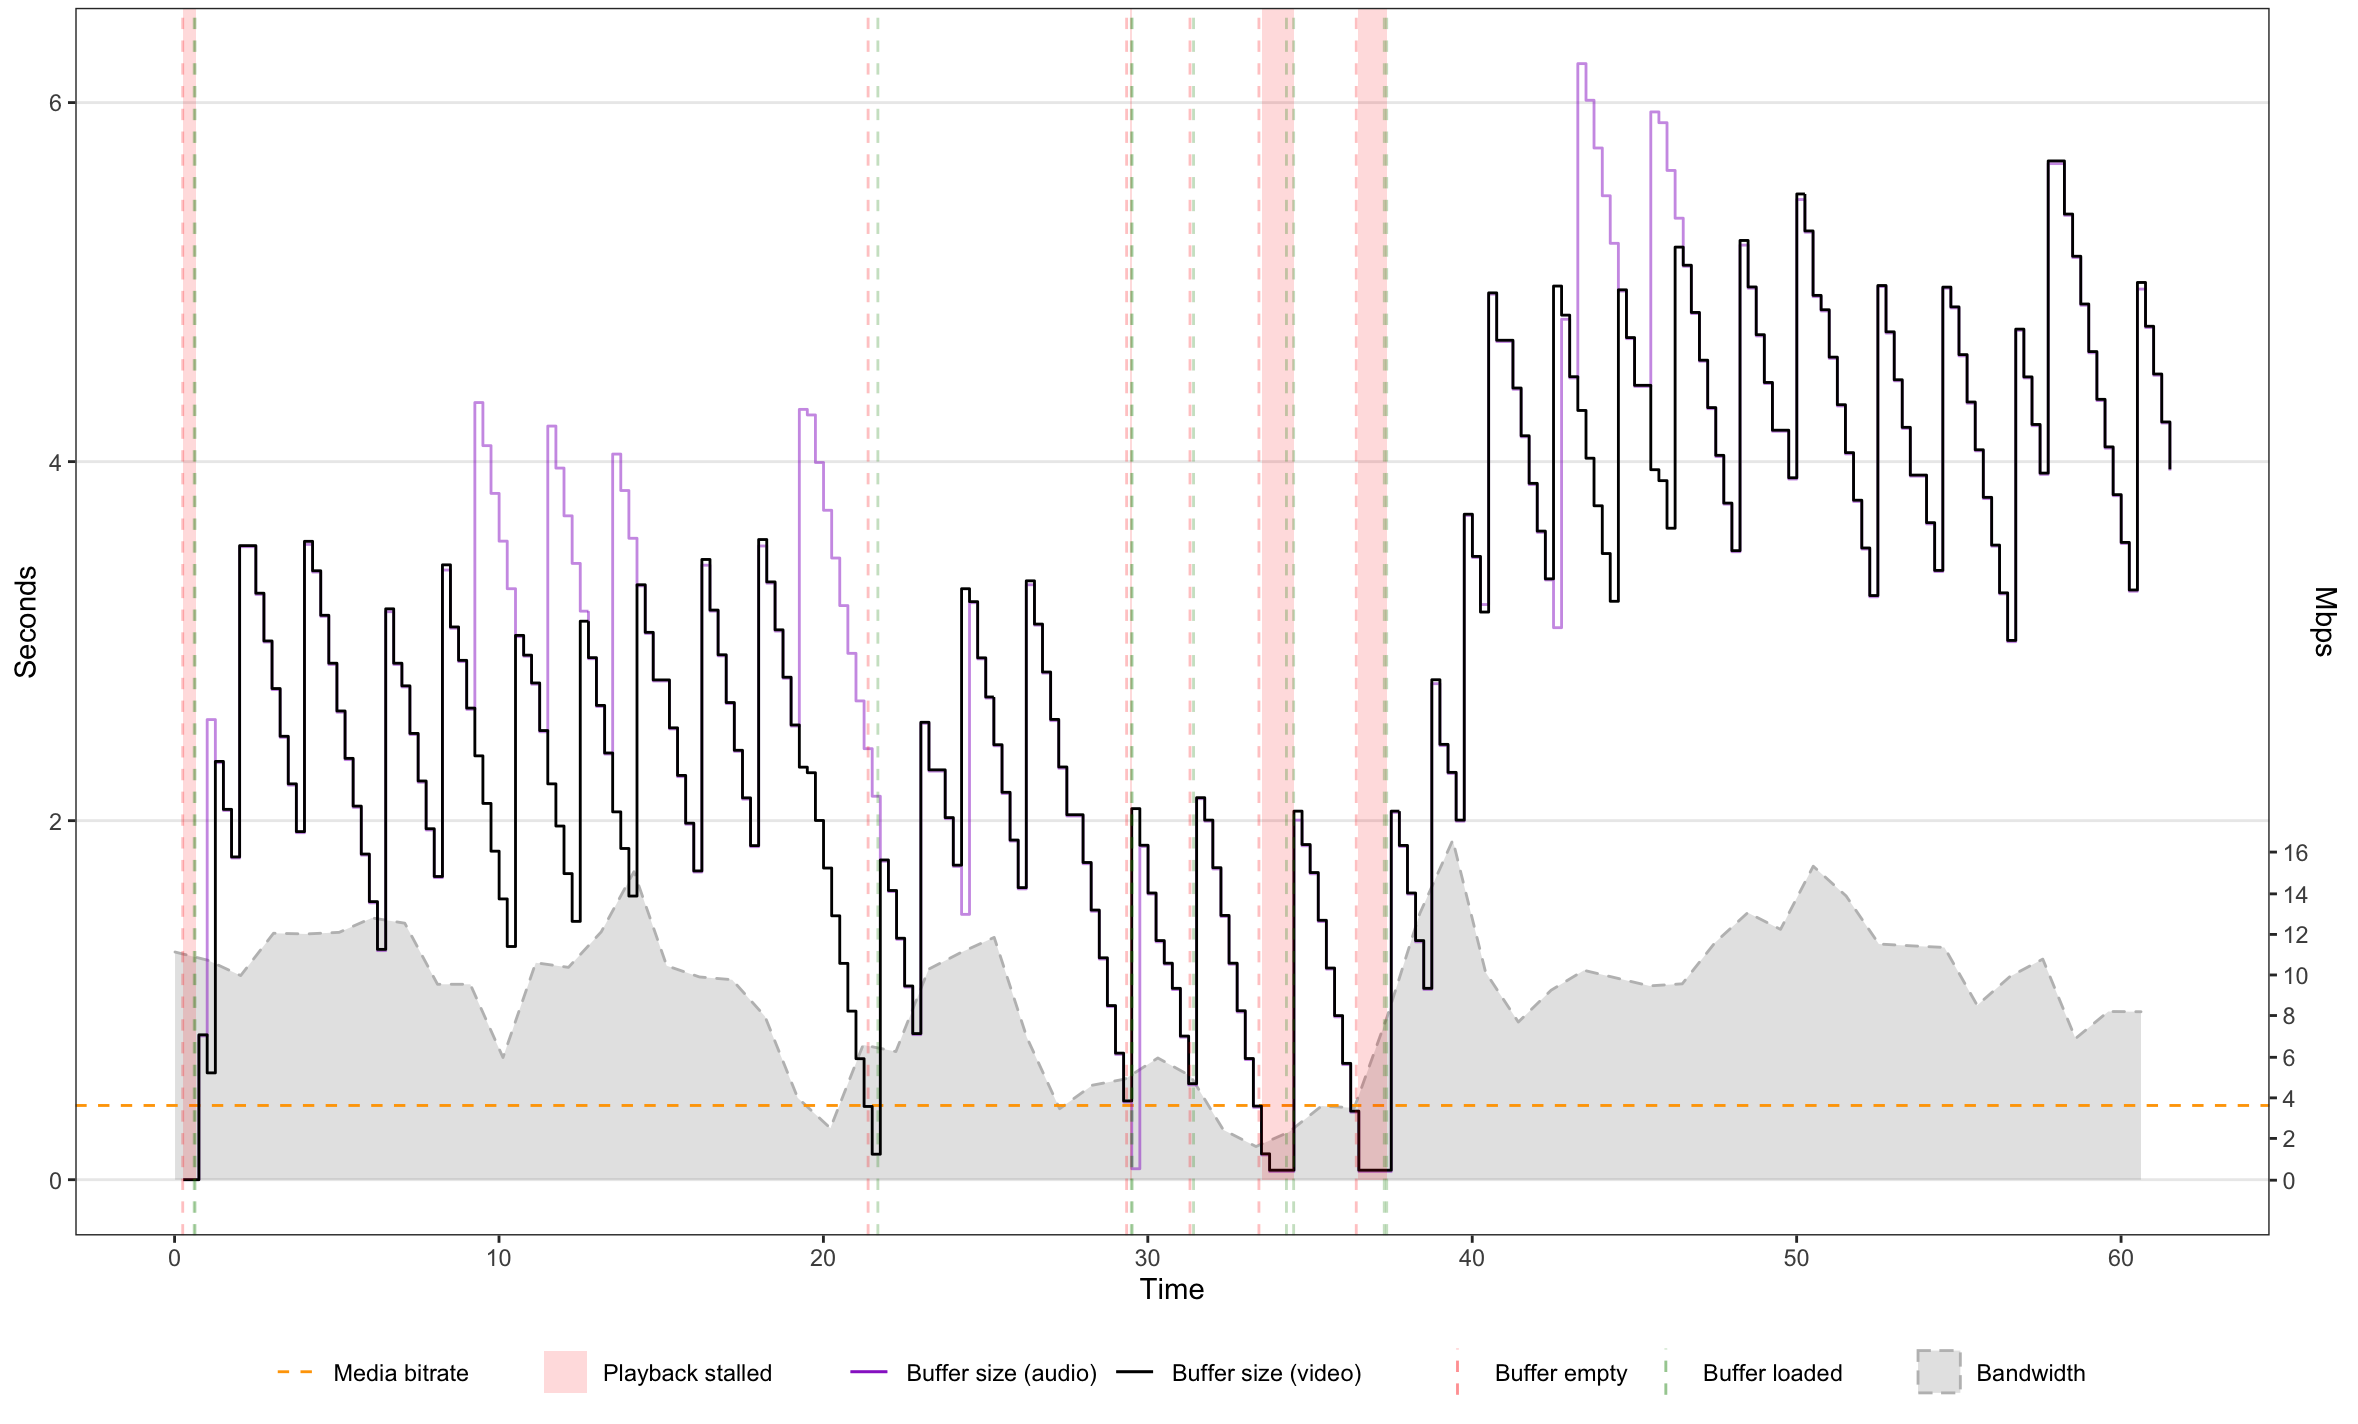
\includegraphics[width=0.9\textwidth]{res/eval_nonabr_lte_h3.png}
    \caption{Caption}
    \label{fig:eval_nonabr_lte_h3}
\end{figure}

What we can observe from the plot is that for the first 30 seconds the bandwidth is generally above the bitrate of the media, and therefore the buffer can be filled properly most of the time. One thing we can already observe is that the audio buffer is sometimes filled with more seconds of data than the video buffer. This happens because the video and audio tracks are unmuxed and can therefore be downloaded independently by the player/browser. Depending on the HTTP response scheduling, the audio segment might arrive before the video segment, or vice versa.

In the first half of the experiment, we can also notice a couple of cases where the player struggles to fill the video buffer in time. For example, just after second 20 the video buffer actually becomes empty for a very short period of time. As we will see later, in practice this kind of event does not necessarily produce a playback stall due to the way Chromium handles empty buffers.

At about second 30, the bandwidth starts to become very limited and goes below 3.5 Mbps for a few seconds. The video and audio buffers quickly deplete, empty buffer events are emitted, and the playback stalls. This happens twice, as can be seen by the two red areas.

When the network bandwidth grows again, the buffers are filled. One thing to note is that the buffer length now contains about one segment more on average (it is in fact closer to 4 seconds than to 2). This happens because the delay introduced by the stall caused the playback to get behind with respect to the edge of the playlist, and therefore there is now an additional segment that can be loaded in advance.

The effect of this behavior can be better seen in the \textbf{live latency plot}, shown in Figure \ref{fig:eval_nonabr_lte_h3_latency}. In correspondence of the playback stalls, the live latency grows from about 4.5 to 5.5 seconds, and then to 6.5 seconds (in total, a 2-second segment more).

\begin{figure}[h]
    \centering
    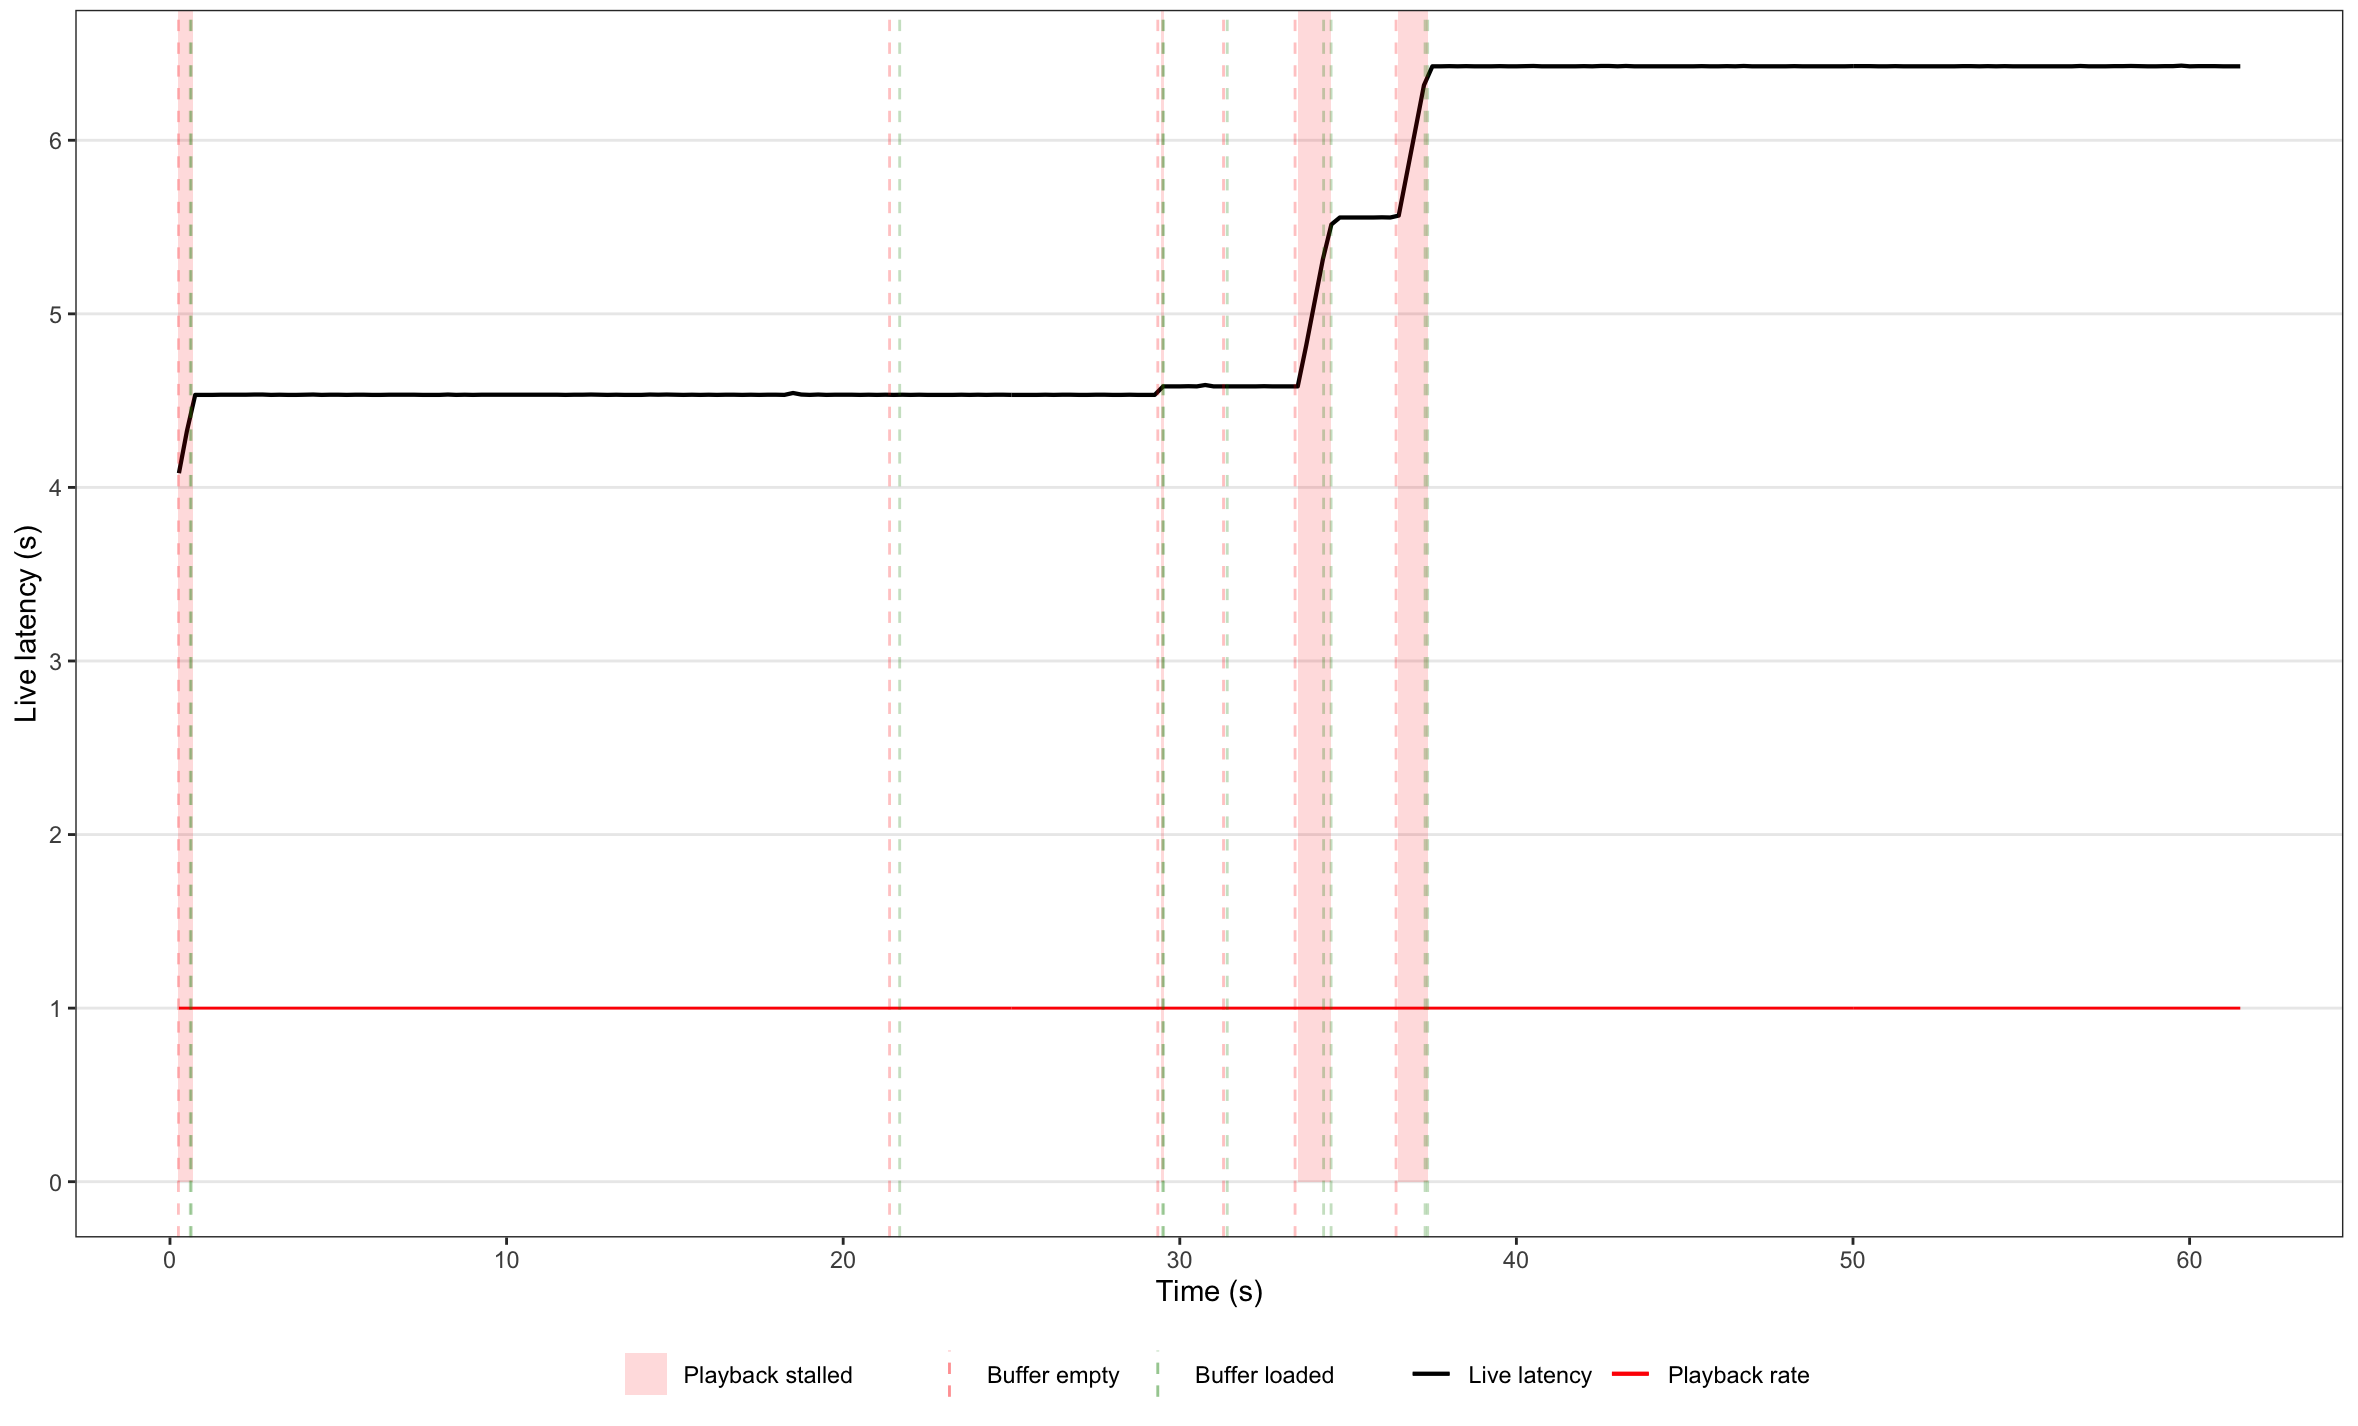
\includegraphics[width=0.9\textwidth]{res/eval_nonabr_lte_h3_latency.png}
    \caption{Caption}
    \label{fig:eval_nonabr_lte_h3_latency}
\end{figure}

Finally, if we observe the \textbf{waterfall diagram} (Figure \ref{fig:eval_nonabr_lte_h3_waterfall}), an interesting and perhaps unexpected behavior can be observed. Intuitively, we would expect requests for audio segments to always take less time than video segments. In fact, while a single video segment can be as large as 6-700 KiB, the audio segment is usually about 30 KiB in size. This is usually between 10 and 20 times smaller than video. However, the waterfall shows that, while sometimes the loading of the audio segment takes very little time, the loading of the audio segments often takes as long as the video.

\begin{figure}[h]
    \centering
    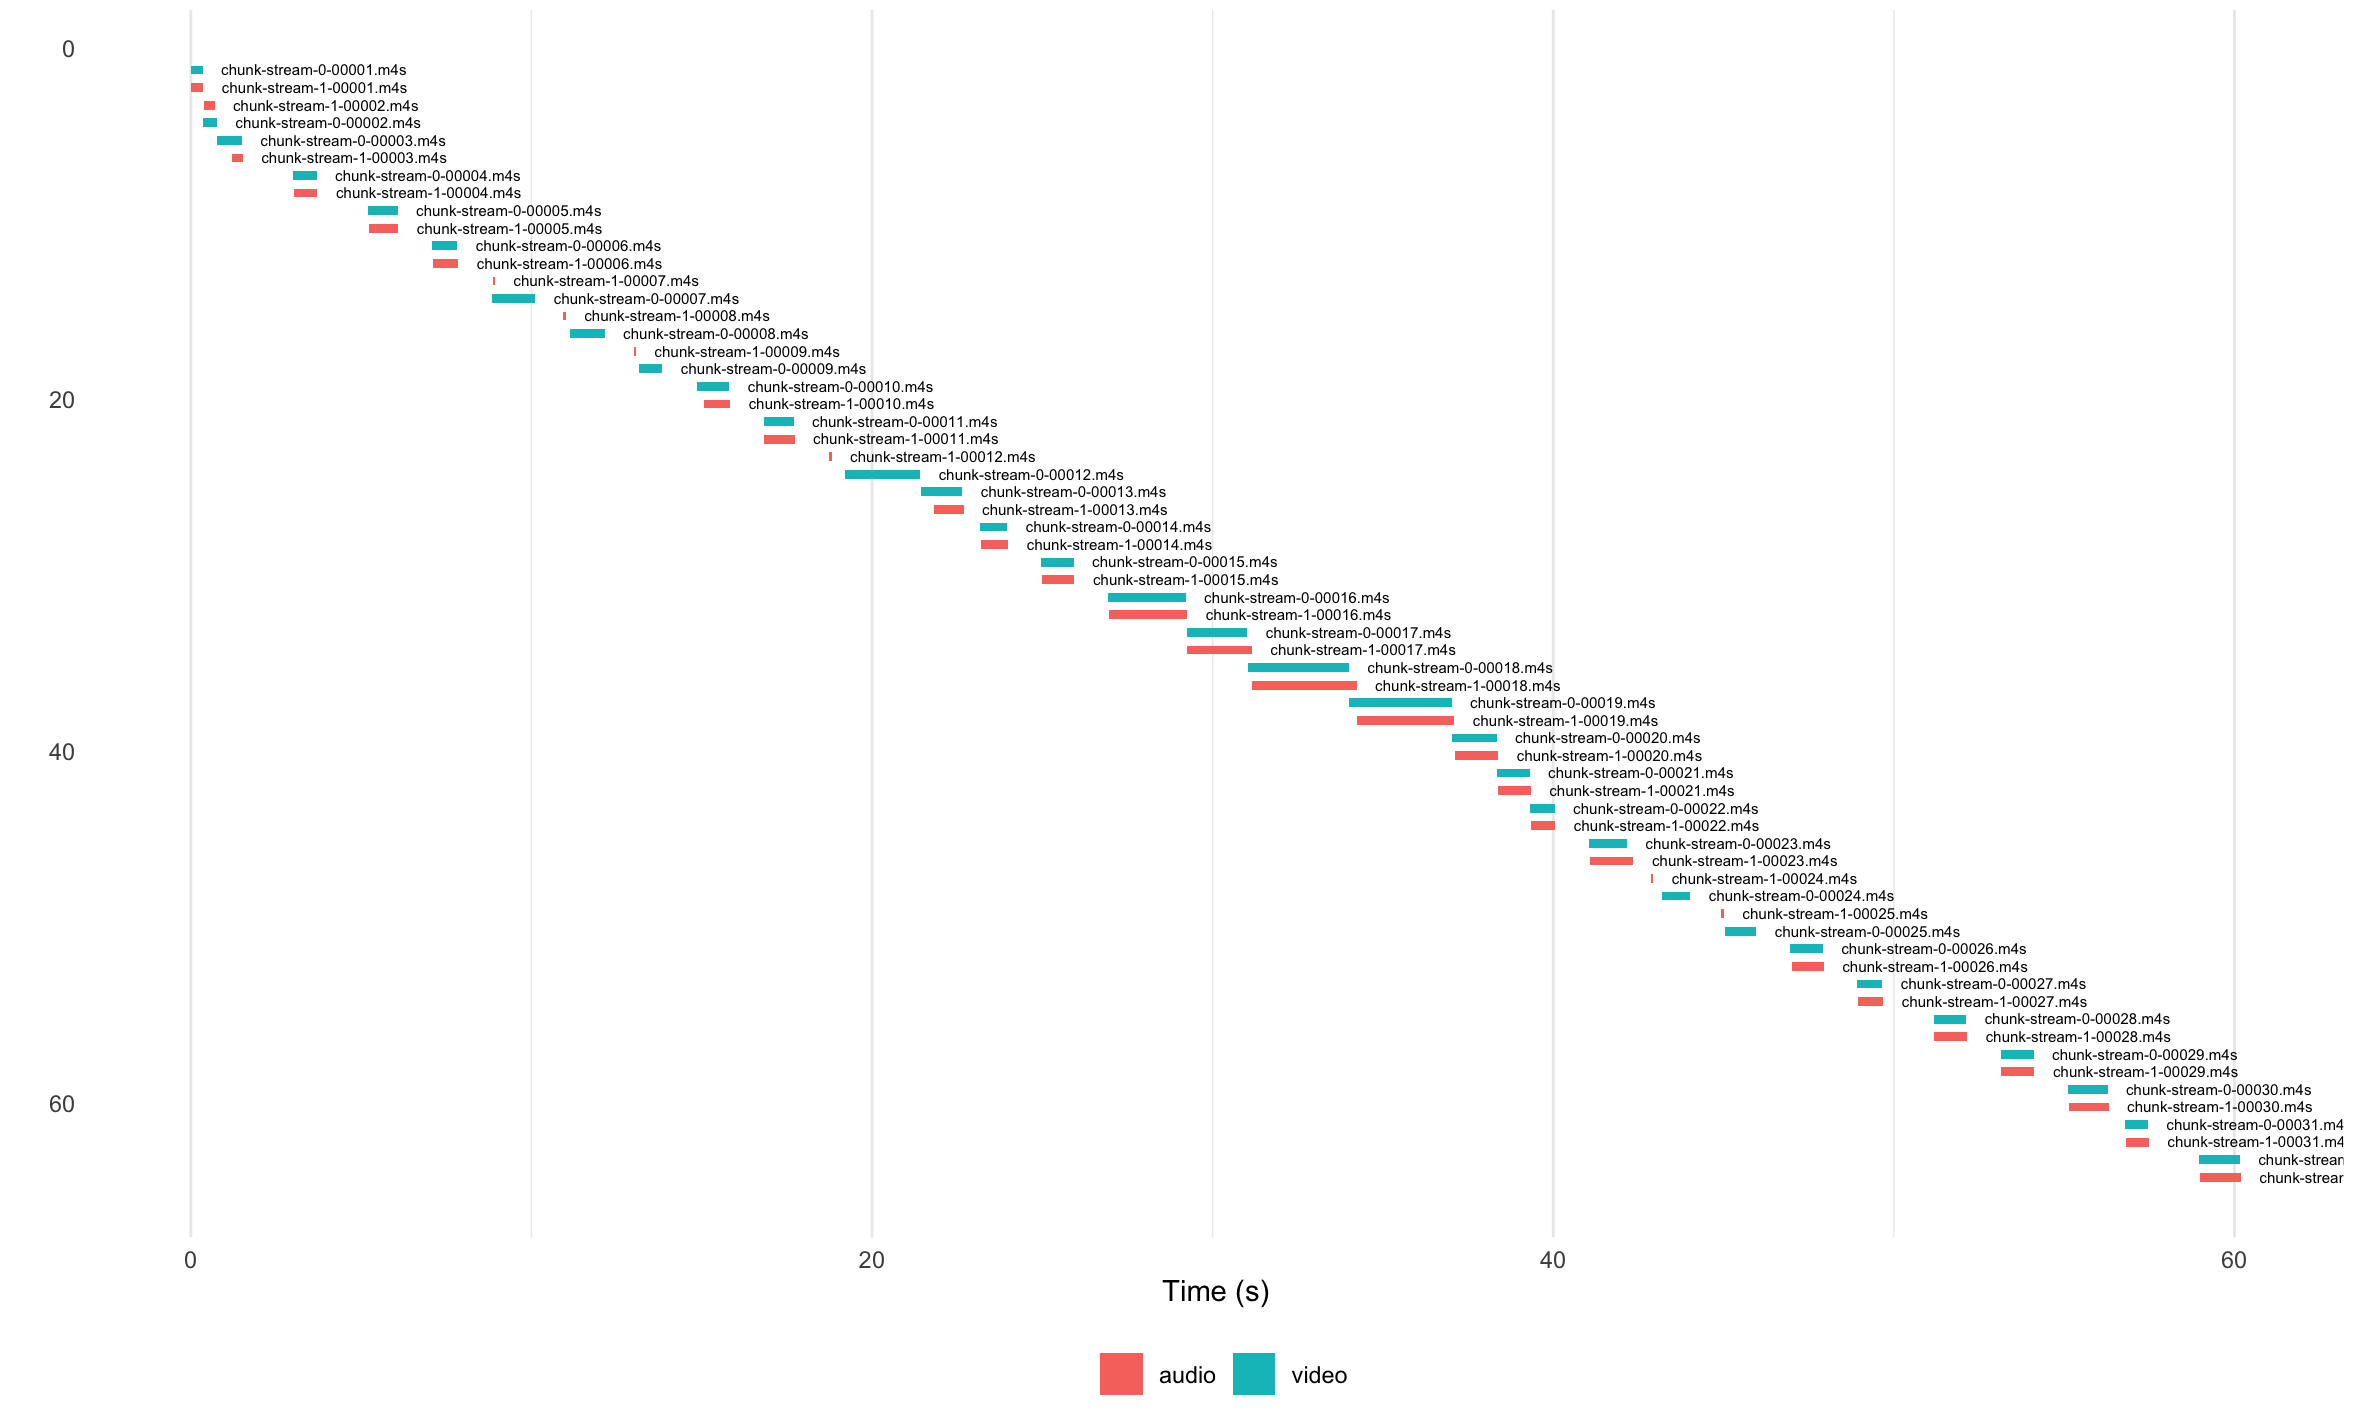
\includegraphics[width=0.9\textwidth]{res/eval_nonabr_lte_h3_waterfall.png}
    \caption{Caption}
    \label{fig:eval_nonabr_lte_h3_waterfall}
\end{figure}

This behavior hints at a suboptimal scheduling strategy of HTTP requests over the QUIC connection, so we decided to investigate. We used the \textbf{NetLog dump} feature of Chromium (Section \ref{sec:bg/http3/tools}) to generate an export of network traffic, which also contains detailed information about QUIC connections and streams. We then analyzed the dump file with \textbf{qvis}.

One of the visualization tools provided by \textbf{qvis} is the multiplexing view, where the multiplexing of the streams at the QUIC level is represented both as a flow/timeline and as a waterfall (Figure \ref{fig:eval_noabr_qvis1}). The flow representation shows the sequence of QUIC packets that the client received. Each packet is colored with a different color depending on the stream to which it belongs. The waterfall view shows the same data as a waterfall chart, where each stream has its own row, and the horizontal segments represent the time intervals in which the stream was actively being transferred.

In our case, what we can clearly see in the multiplexing diagrams, especially in the waterfall, is that the streams are transmitted almost sequentially. In fact, there is almost no preemption, and most streams get to use the entire channel for transmission until all data is received.

\begin{figure}[h]
    \centering
    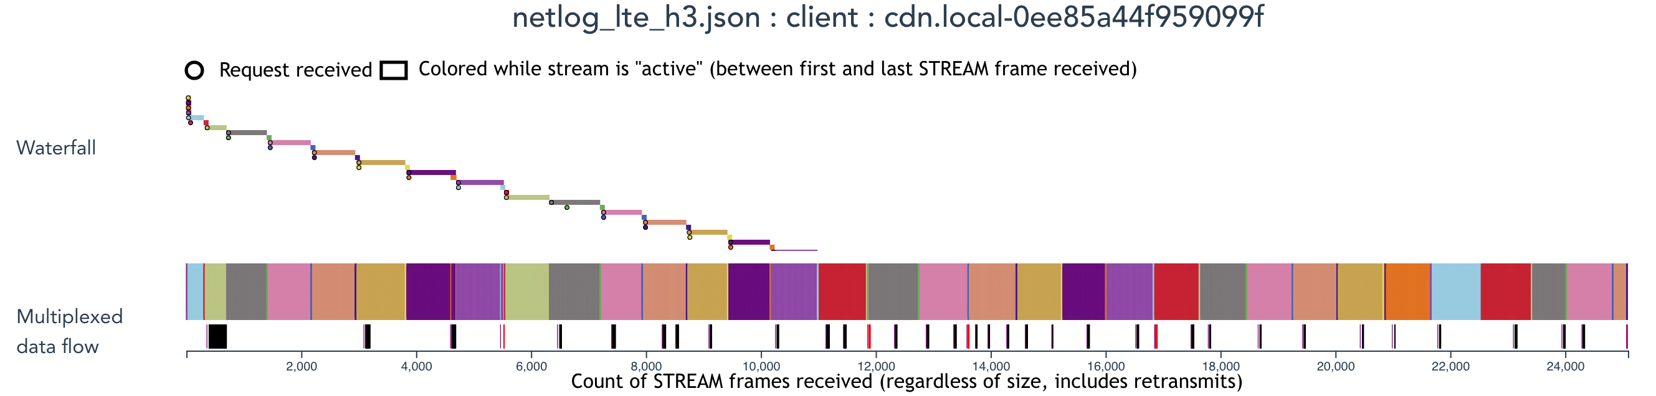
\includegraphics[width=0.9\textwidth]{res/eval_nonabr_qvis1.png}
    \caption{Caption}
    \label{fig:eval_noabr_qvis1}
\end{figure}

However, an interesting fact to observe is that the data flow is not entirely sequential. As Figure \ref{fig:eval_noabr_qvis2} shows, there is a recurring pattern of streams/requests that start and are immediately suspended to give bandwidth to another stream on the QUIC connection.

This behavior explains what we were seeing in the segments requests waterfall in Figure \ref{fig:eval_nonabr_lte_h3_waterfall}. Requests for audio and video segments often start at the same time; however, the transfer of the audio segment is almost immediately preempted to give priority to the video segment. The audio segment transfer is then completed after the video segment is completely downloaded.

This behavior is not ideal, because an audio segment is always much smaller than a video segment and thus could benefit from being received by the client earlier, as we will see in the next section. The next section will also compare how this same setup performs with HTTP/2 and HTTP/1.1, showing that the scheduling scheme that was observed seems to be specific to HTTP/3, or at least to the HTTP/3 implementation that we are relying on in this testbed.

The takeaway result of this analysis is that we cannot rely on HTTP/3 implementations to always know the best strategy for request prioritization. Instead, it is also the client/browser's responsibility to implement optimizations so that the prioritization strategy is meaningful.

The prioritization strategy could derive from browser heuristics that are applied globally for all websites, as we mentioned in Section \ref{sec:bg/http2}, but it could also be explicitly requested by developers with the use of priorities, as we explained in Section \ref{sec:eval/browsers/priorities}.

\begin{figure}[h]
    \centering
    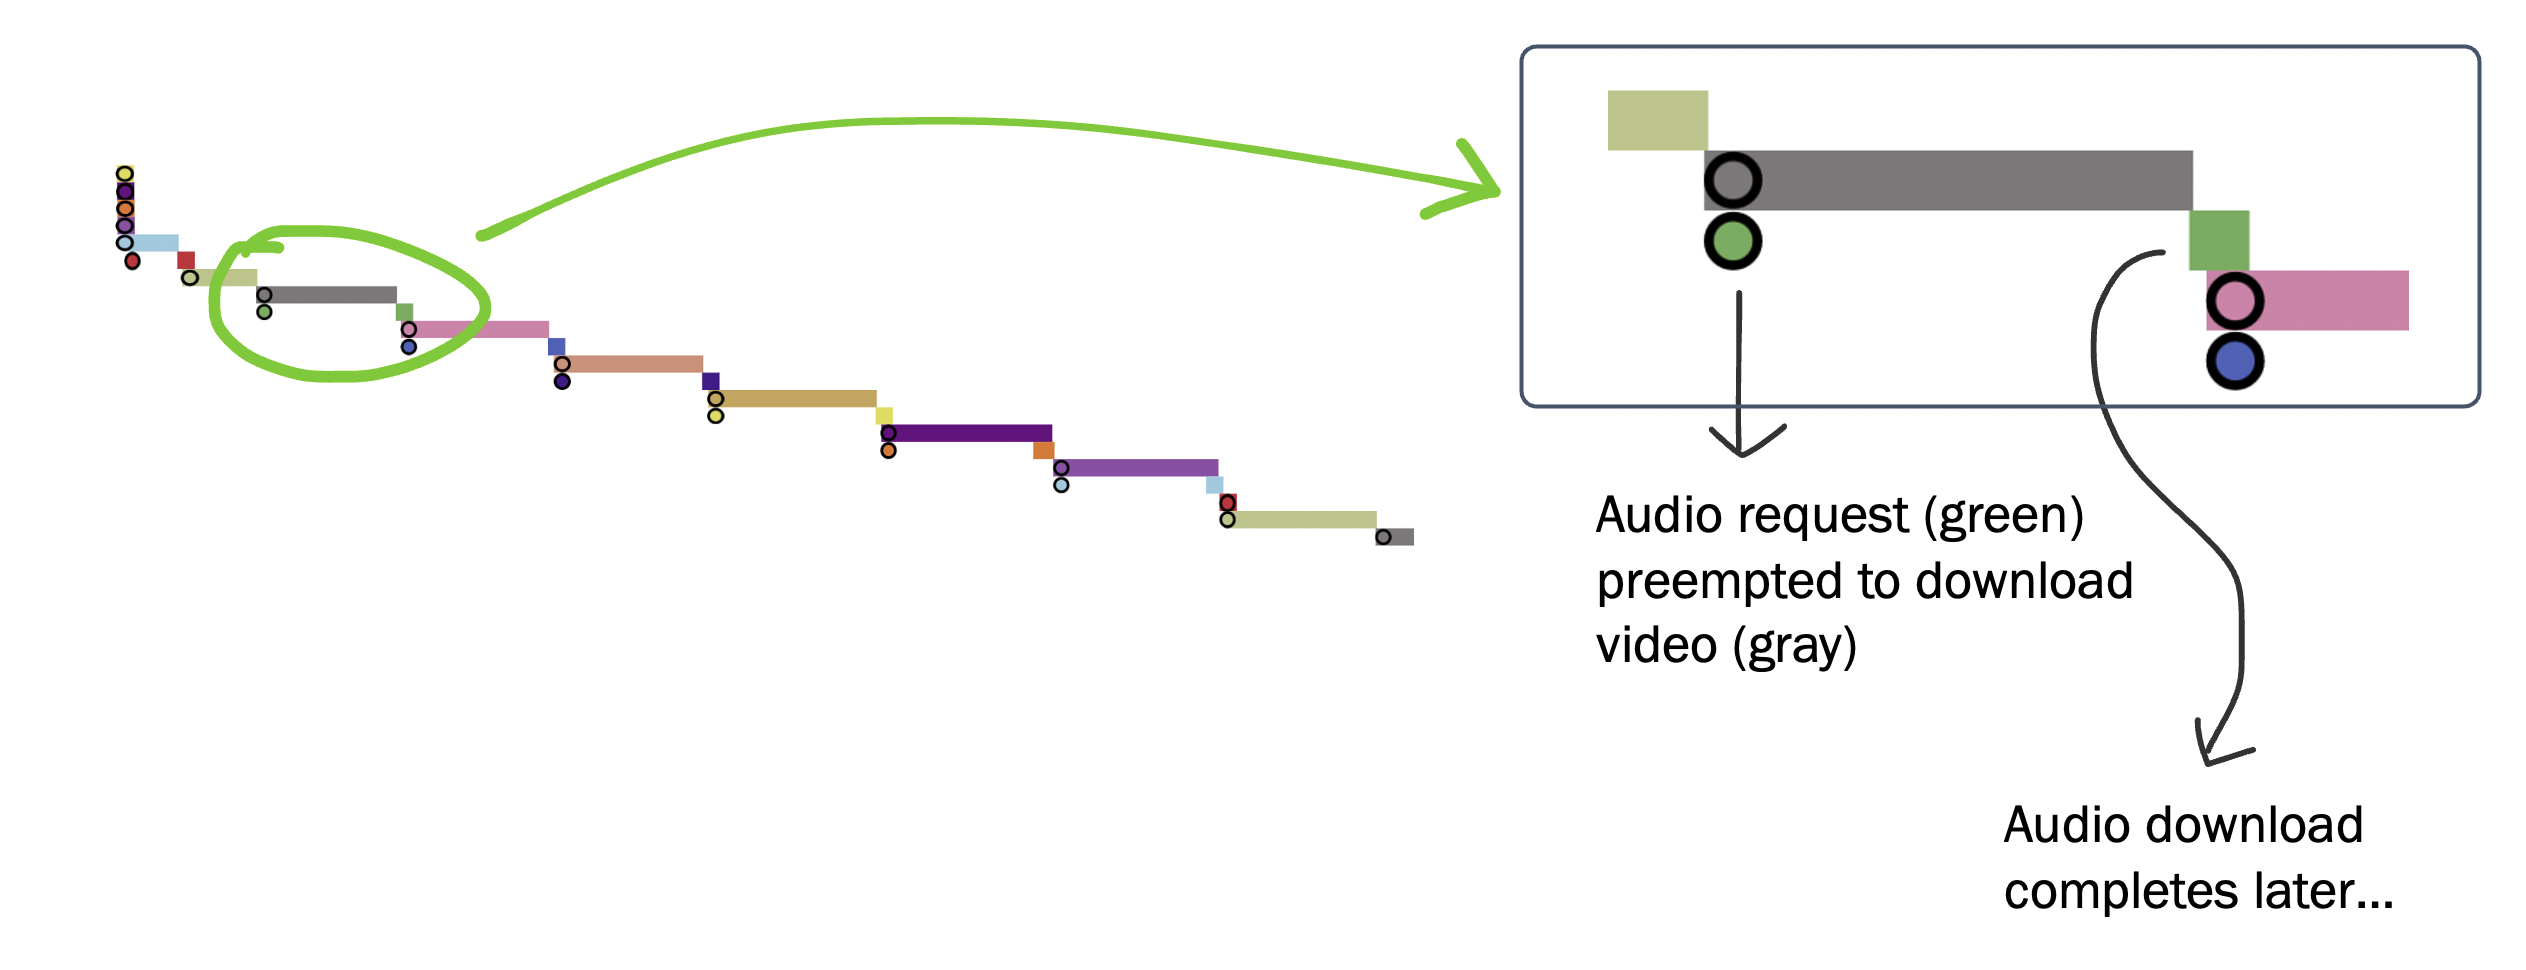
\includegraphics[width=0.9\textwidth]{res/eval_nonabr_qvis2.png}
    \caption{Caption}
    \label{fig:eval_noabr_qvis2}
\end{figure}

\subsubsection{Comparison across HTTP versions}
\label{sec:eval/non-abr/http-versions}

As we have seen, the emulation over HTTP/3 shows that priorities are not consistent, even in the same run. We will now see how HTTP/2 and HTTP/1.1 behave and compare the results.

Let us start from \textbf{HTTP/2}. Figure \ref{fig:eval_nonabr_lte_h2_buffer} shows the buffer health plot for an experiment execution based on HTTP/2. The rest of the settings remained the same. As we can easily see, the behavior is quite different from HTTP/3. First, the audio buffer is always larger than the video. This means that the audio segments are consistently loaded before the video buffer. The waterfall in Figure \ref{fig:eval_nonabr_lte_h2_waterfall} confirms that this is because the audio segments are loaded much faster, as we would expect, and the loading of the video segments does not delay the audio. This behavior probably derives from a different prioritization strategy, implemented by the browser or driven by the HTTP/2 server implementation.

The other thing that we can observe is that there are no playback stalls, apart from the initial loading, even if the video buffer is almost empty for several seconds in the middle of the emulation. This behavior derives from the fact that the browser is capable of playing the audio data even if the video is not available, for up to 3 seconds. This particular \textbf{buffer underflow behavior} is specific to Chromium and is officially documented.\footnote{\url{https://www.chromium.org/audio-video/#how-the-does-buffering-work}} Obviously, it can only work when audio and video data is appended to the MSE \texttt{SourceBuffer} independently; therefore, in practice it can only happen when using unmuxed video and audio tracks, as is in our case.

Although Chromium's underflow behavior might not be the expected experience when streaming on-demand content, since it has the effect of not rendering the video for a few seconds, it is instead particularly suitable for low-latency live streaming. In fact, in this way short time intervals where video data is not available do not cause a stall, and, therefore, do not increase the latency of the live streams. While the video is frozen due to a slow loading segment, the audio will continue to play.

\begin{figure}[h]
	\centering
	
	\begin{subfigure}[t]{0.45\textwidth}
		\centering
		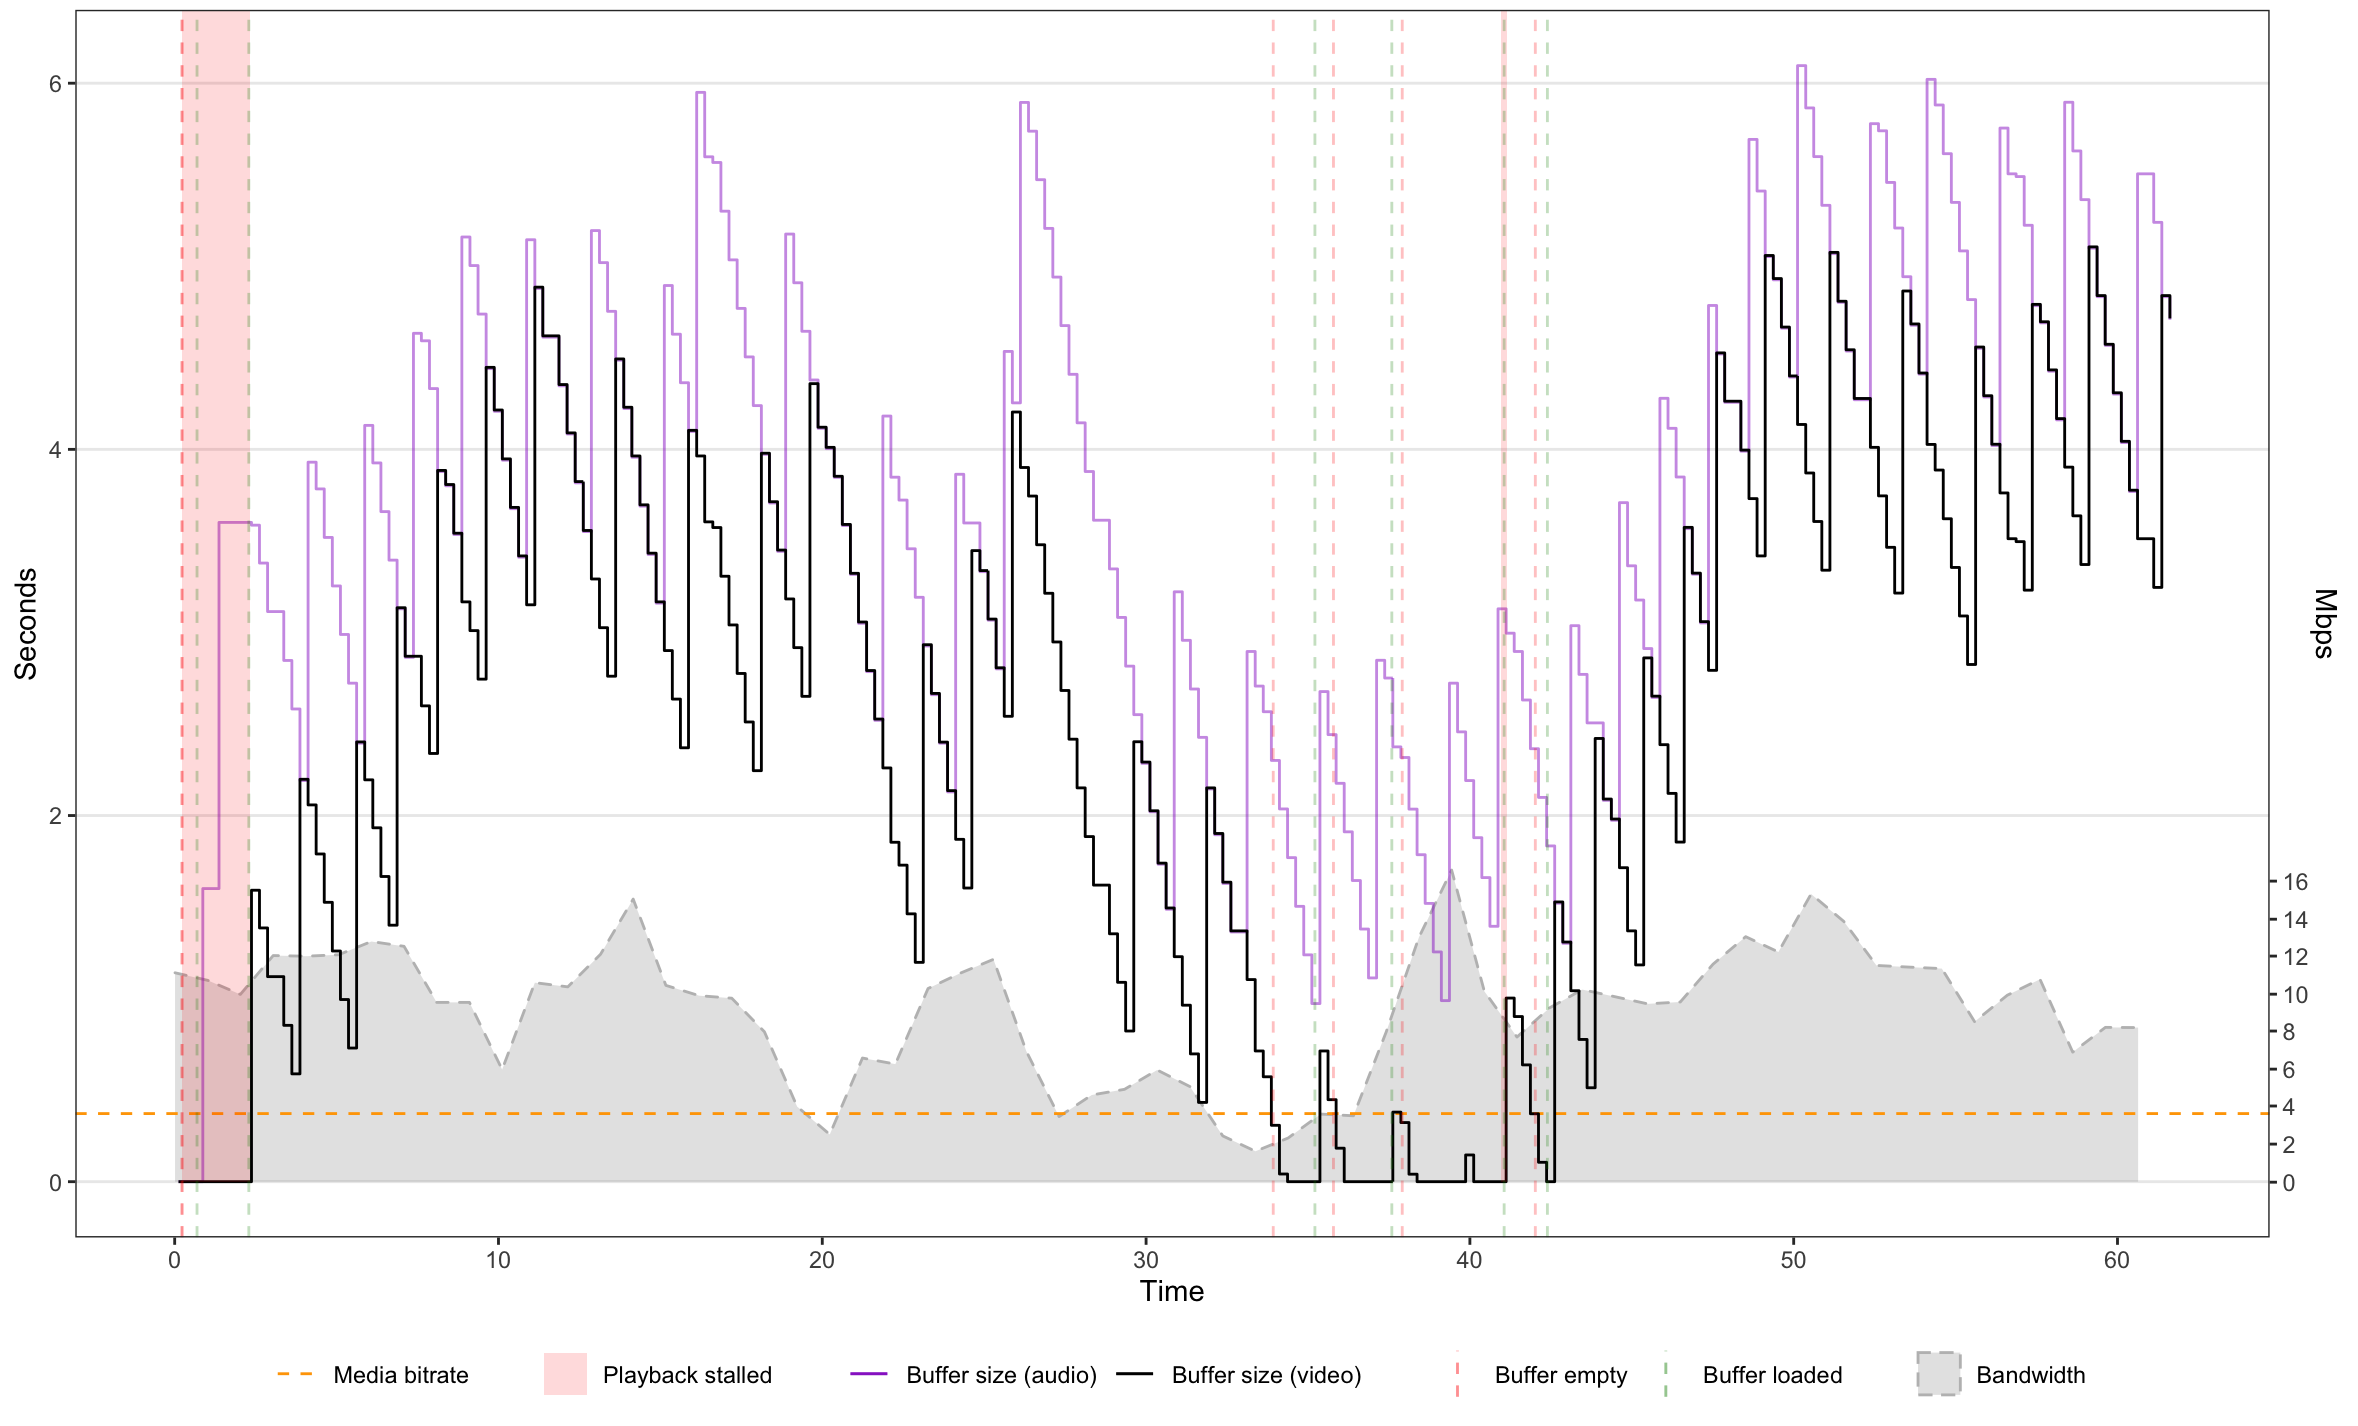
\includegraphics[width=\textwidth]{res/eval_nonabr_lte_h2.png}
		\caption{Caption}
		\label{fig:eval_nonabr_lte_h2_buffer}
	\end{subfigure}%
	~ 
	\begin{subfigure}[t]{0.45\textwidth}
		\centering
		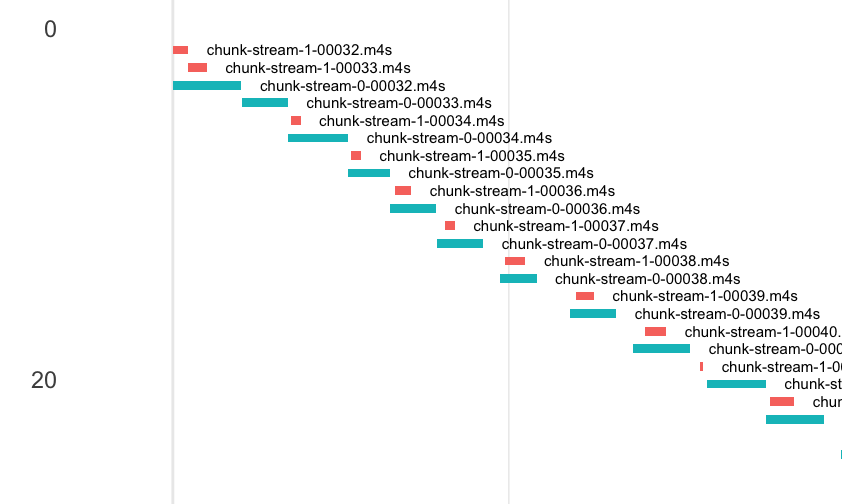
\includegraphics[width=\textwidth]{res/eval_nonabr_lte_h2_waterfall.png}
		\caption{Caption}
		\label{fig:eval_nonabr_lte_h2_waterfall}
	\end{subfigure}
	
	\caption{Caption}
	\label{fig:eval_nonabr_lte_h2}
\end{figure}

Moving on to \textbf{HTTP/1.1}, the behavior that we observed is somewhat similar to HTTP/2. As Figure \ref{fig:eval_nonabr_lte_h1_buffer} shows, the audio buffer is virtually always longer than the video buffer. One thing to note is that there is a playback stall at about 38 seconds, even if the audio buffer contains several seconds of data. This is due to the limitations of the underflow tolerance we have just introduced: Chromium only allows the video track to have missing data for about 3 seconds, after which the playback will stall. We will address this limitation in Section X.

The waterfall diagram for HTTP/1.1, shown in \ref{fig:eval_nonabr_lte_h1_waterfall}, is perhaps even more interesting. It shows that the download of the audio segments, represented in red, is consistently completed in a very short amount of time. Intuitively, the explanation for this phenomenon is that HTTP/1.1 can use multiple independent TCP connections, not performing multiplexing at all. In this way, requests can be distributed among the connections and benefit from a "dedicated" transmission channel.

\begin{figure}[h]
	\centering
	
	\begin{subfigure}[t]{0.45\textwidth}
		\centering
		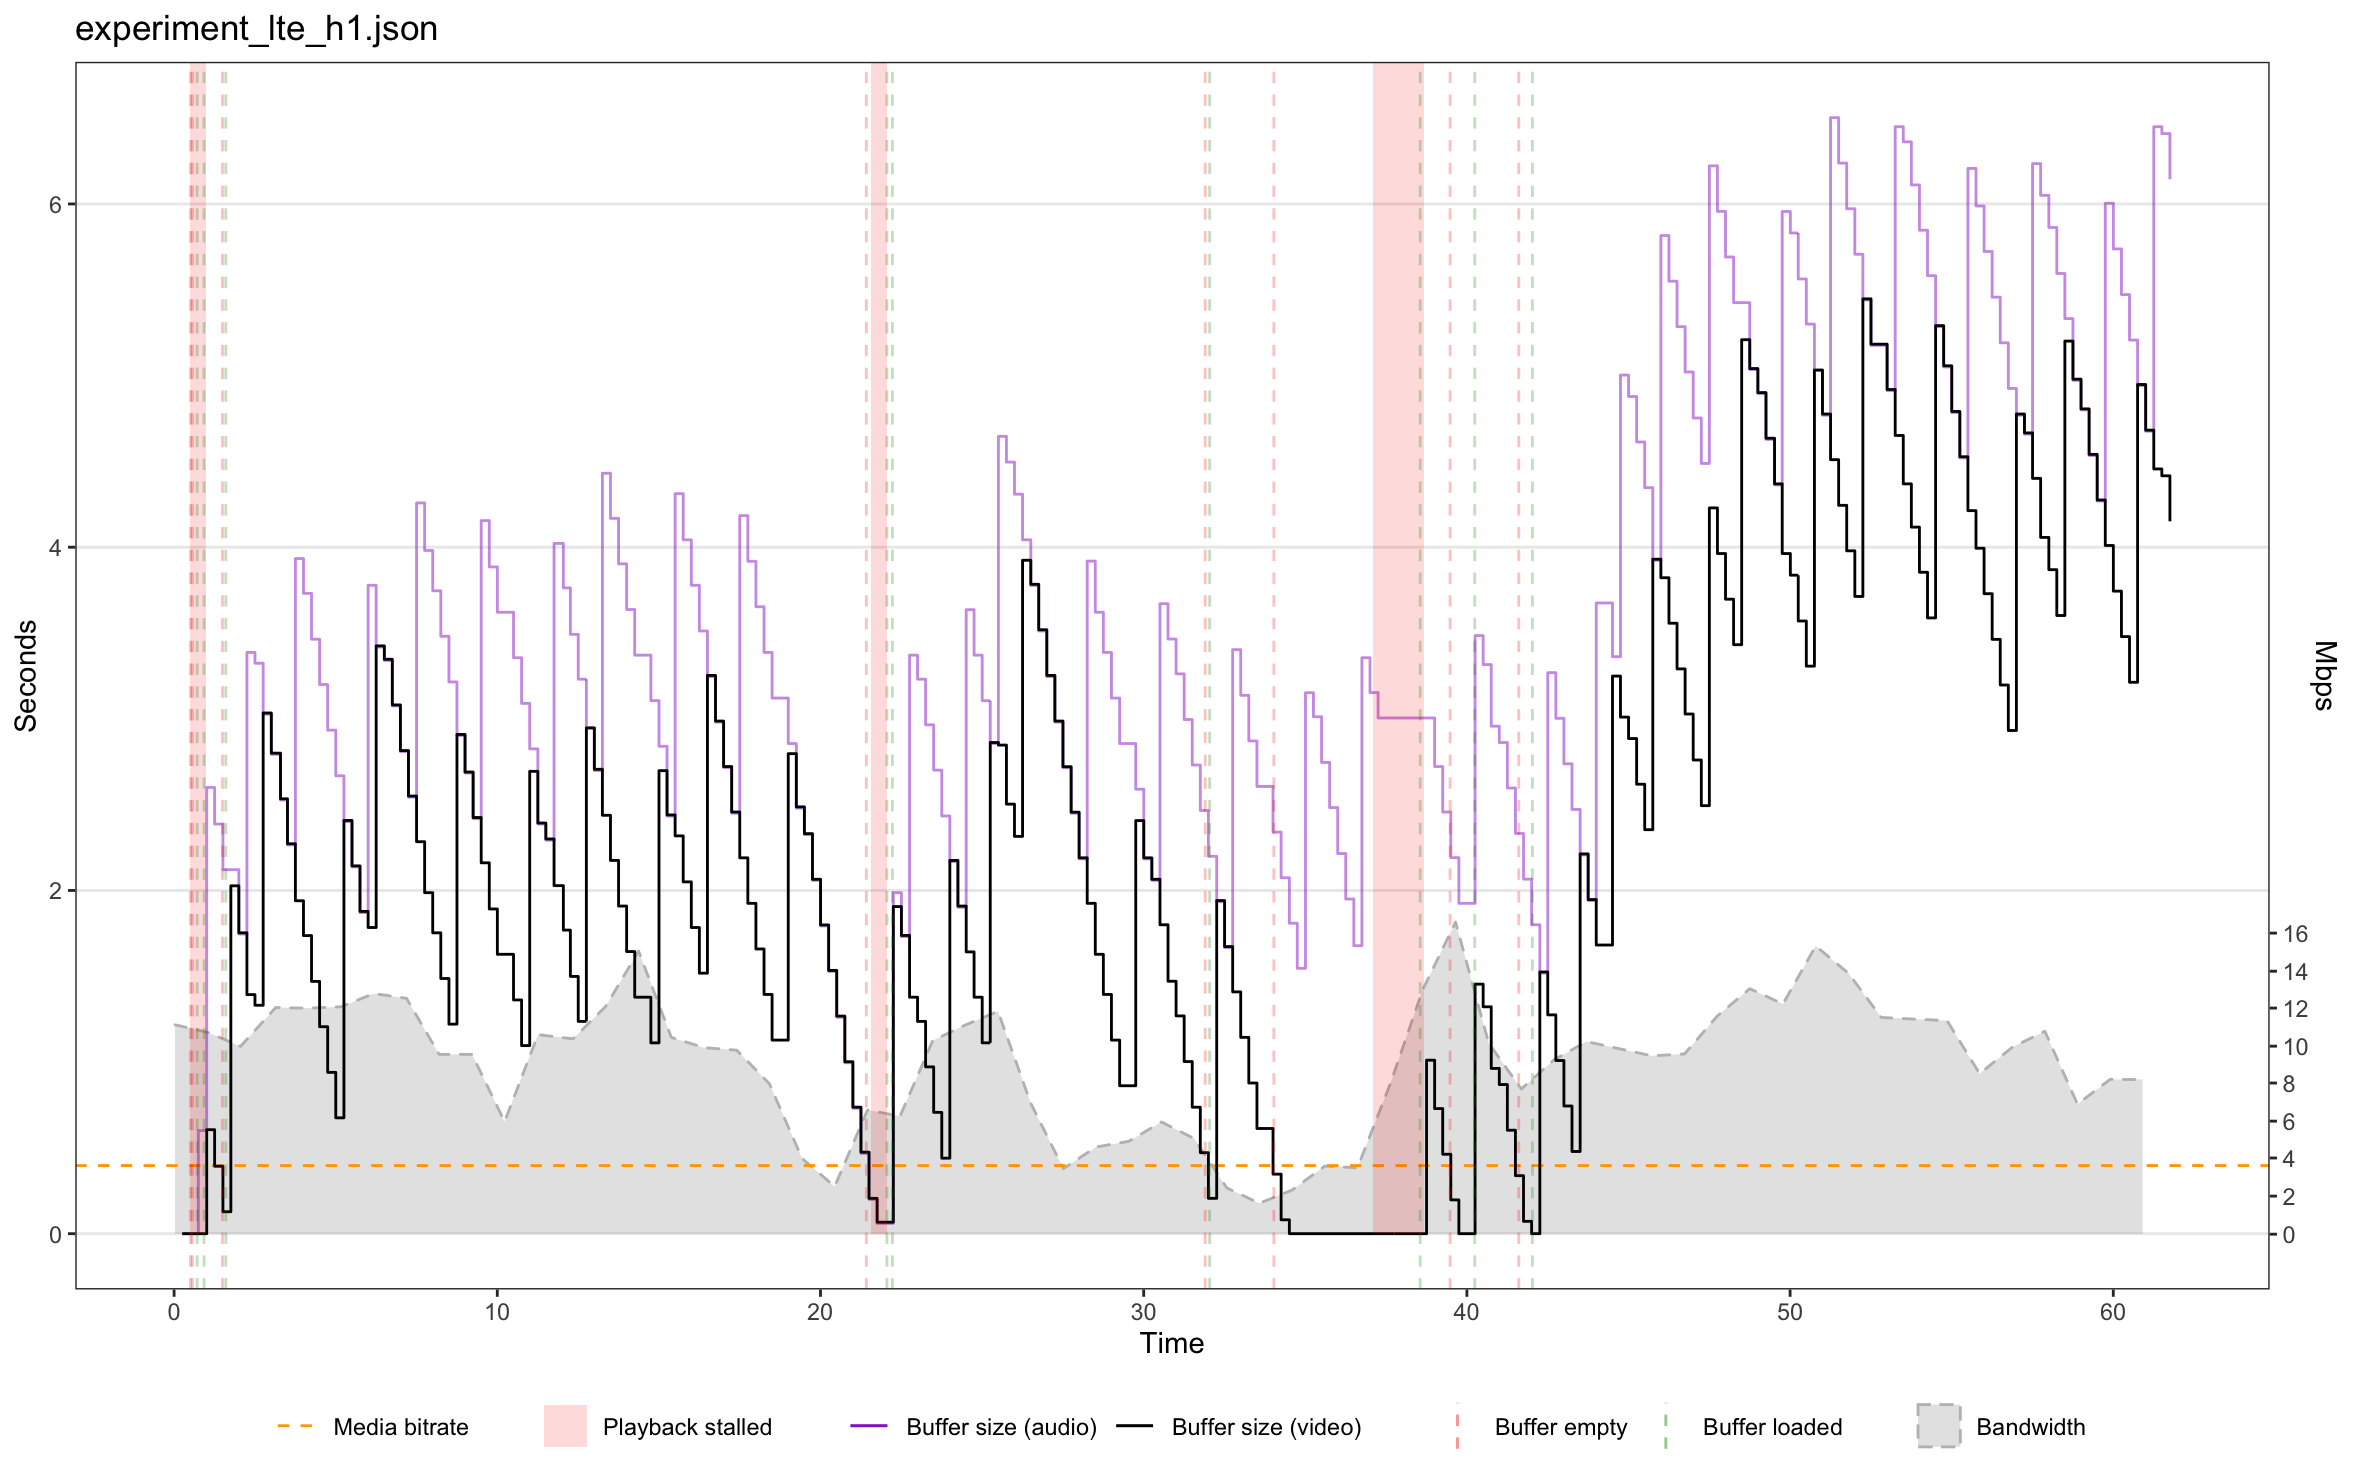
\includegraphics[width=\textwidth]{res/eval_nonabr_lte_h1.png}
		\caption{Caption}
		\label{fig:eval_nonabr_lte_h1_buffer}
	\end{subfigure}%
	~ 
	\begin{subfigure}[t]{0.45\textwidth}
		\centering
		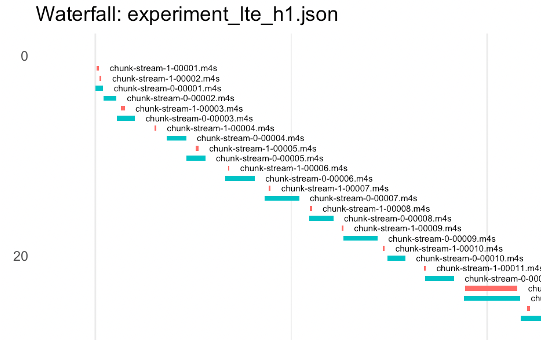
\includegraphics[width=\textwidth]{res/eval_nonabr_lte_h1_waterfall.png}
		\caption{Caption}
		\label{fig:eval_nonabr_lte_h1_waterfall}
	\end{subfigure}
	
	\caption{Caption}
	\label{fig:eval_nonabr_lte_h1}
\end{figure}

These results are surprising. We are seeing that HTTP/2 and HTTP/1.1 appear to offer better scheduling of requests. Incidentally, this also translates into a live streaming experience that has fewer "hard" stalls and where the latency does not increase.

\subsubsection{The need for adaptive bitrate streaming}
\label{sec:eval/non-abr/adaptive}

The experiments mentioned above were conducted with the \texttt{lte} network pattern, where the network bandwidth is most of the time higher than the media bitrate. In the \texttt{hspa+} pattern, the situation is different: the bandwidth is just slightly above the media bitrate and often goes below it. This is pretty clear from Figure \ref{fig:eval_nonabr_hspa+_h3_buffer}, where there are many stalls in all situations where the bandwidth is not enough. The consequence is that the live latency increases during the playback stall periods, reaching 23 seconds as shown in \ref{fig:eval_nonabr_hspa+_h3_waterfall}.

\begin{figure}[h]
	\centering
	
	\begin{subfigure}[t]{0.45\textwidth}
		\centering
		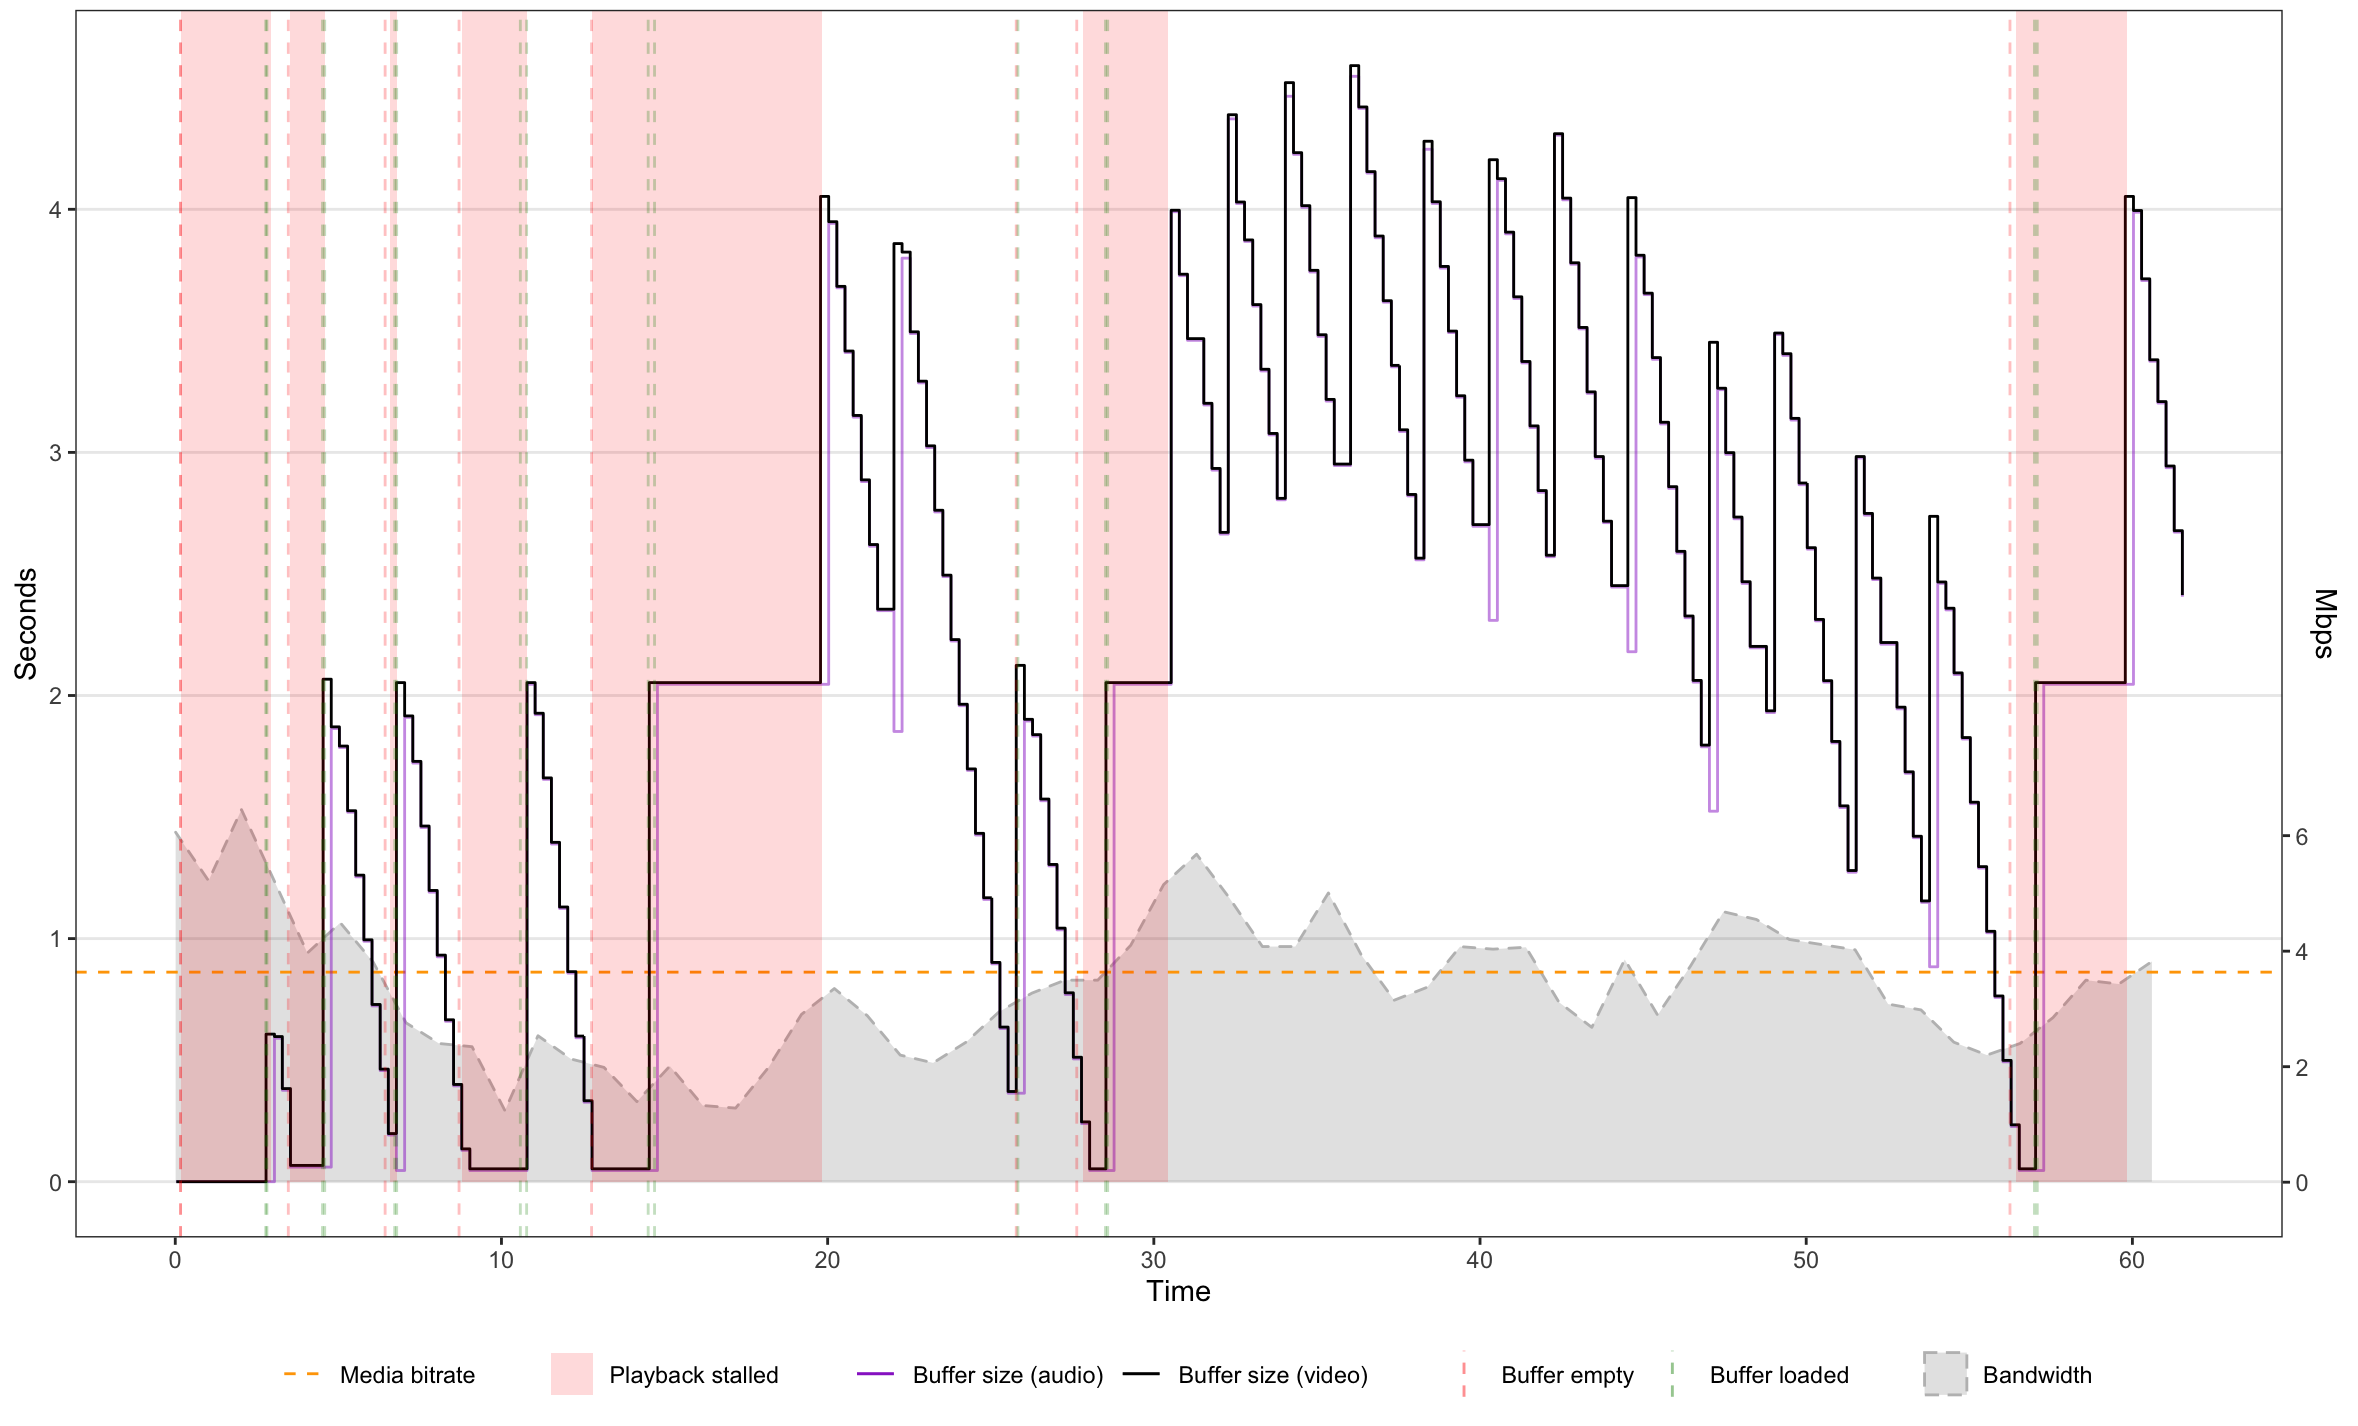
\includegraphics[width=\textwidth]{res/eval_nonabr_hspa+_h3.png}
		\caption{Caption}
		\label{fig:eval_nonabr_hspa+_h3_buffer}
	\end{subfigure}%
	~ 
	\begin{subfigure}[t]{0.45\textwidth}
		\centering
		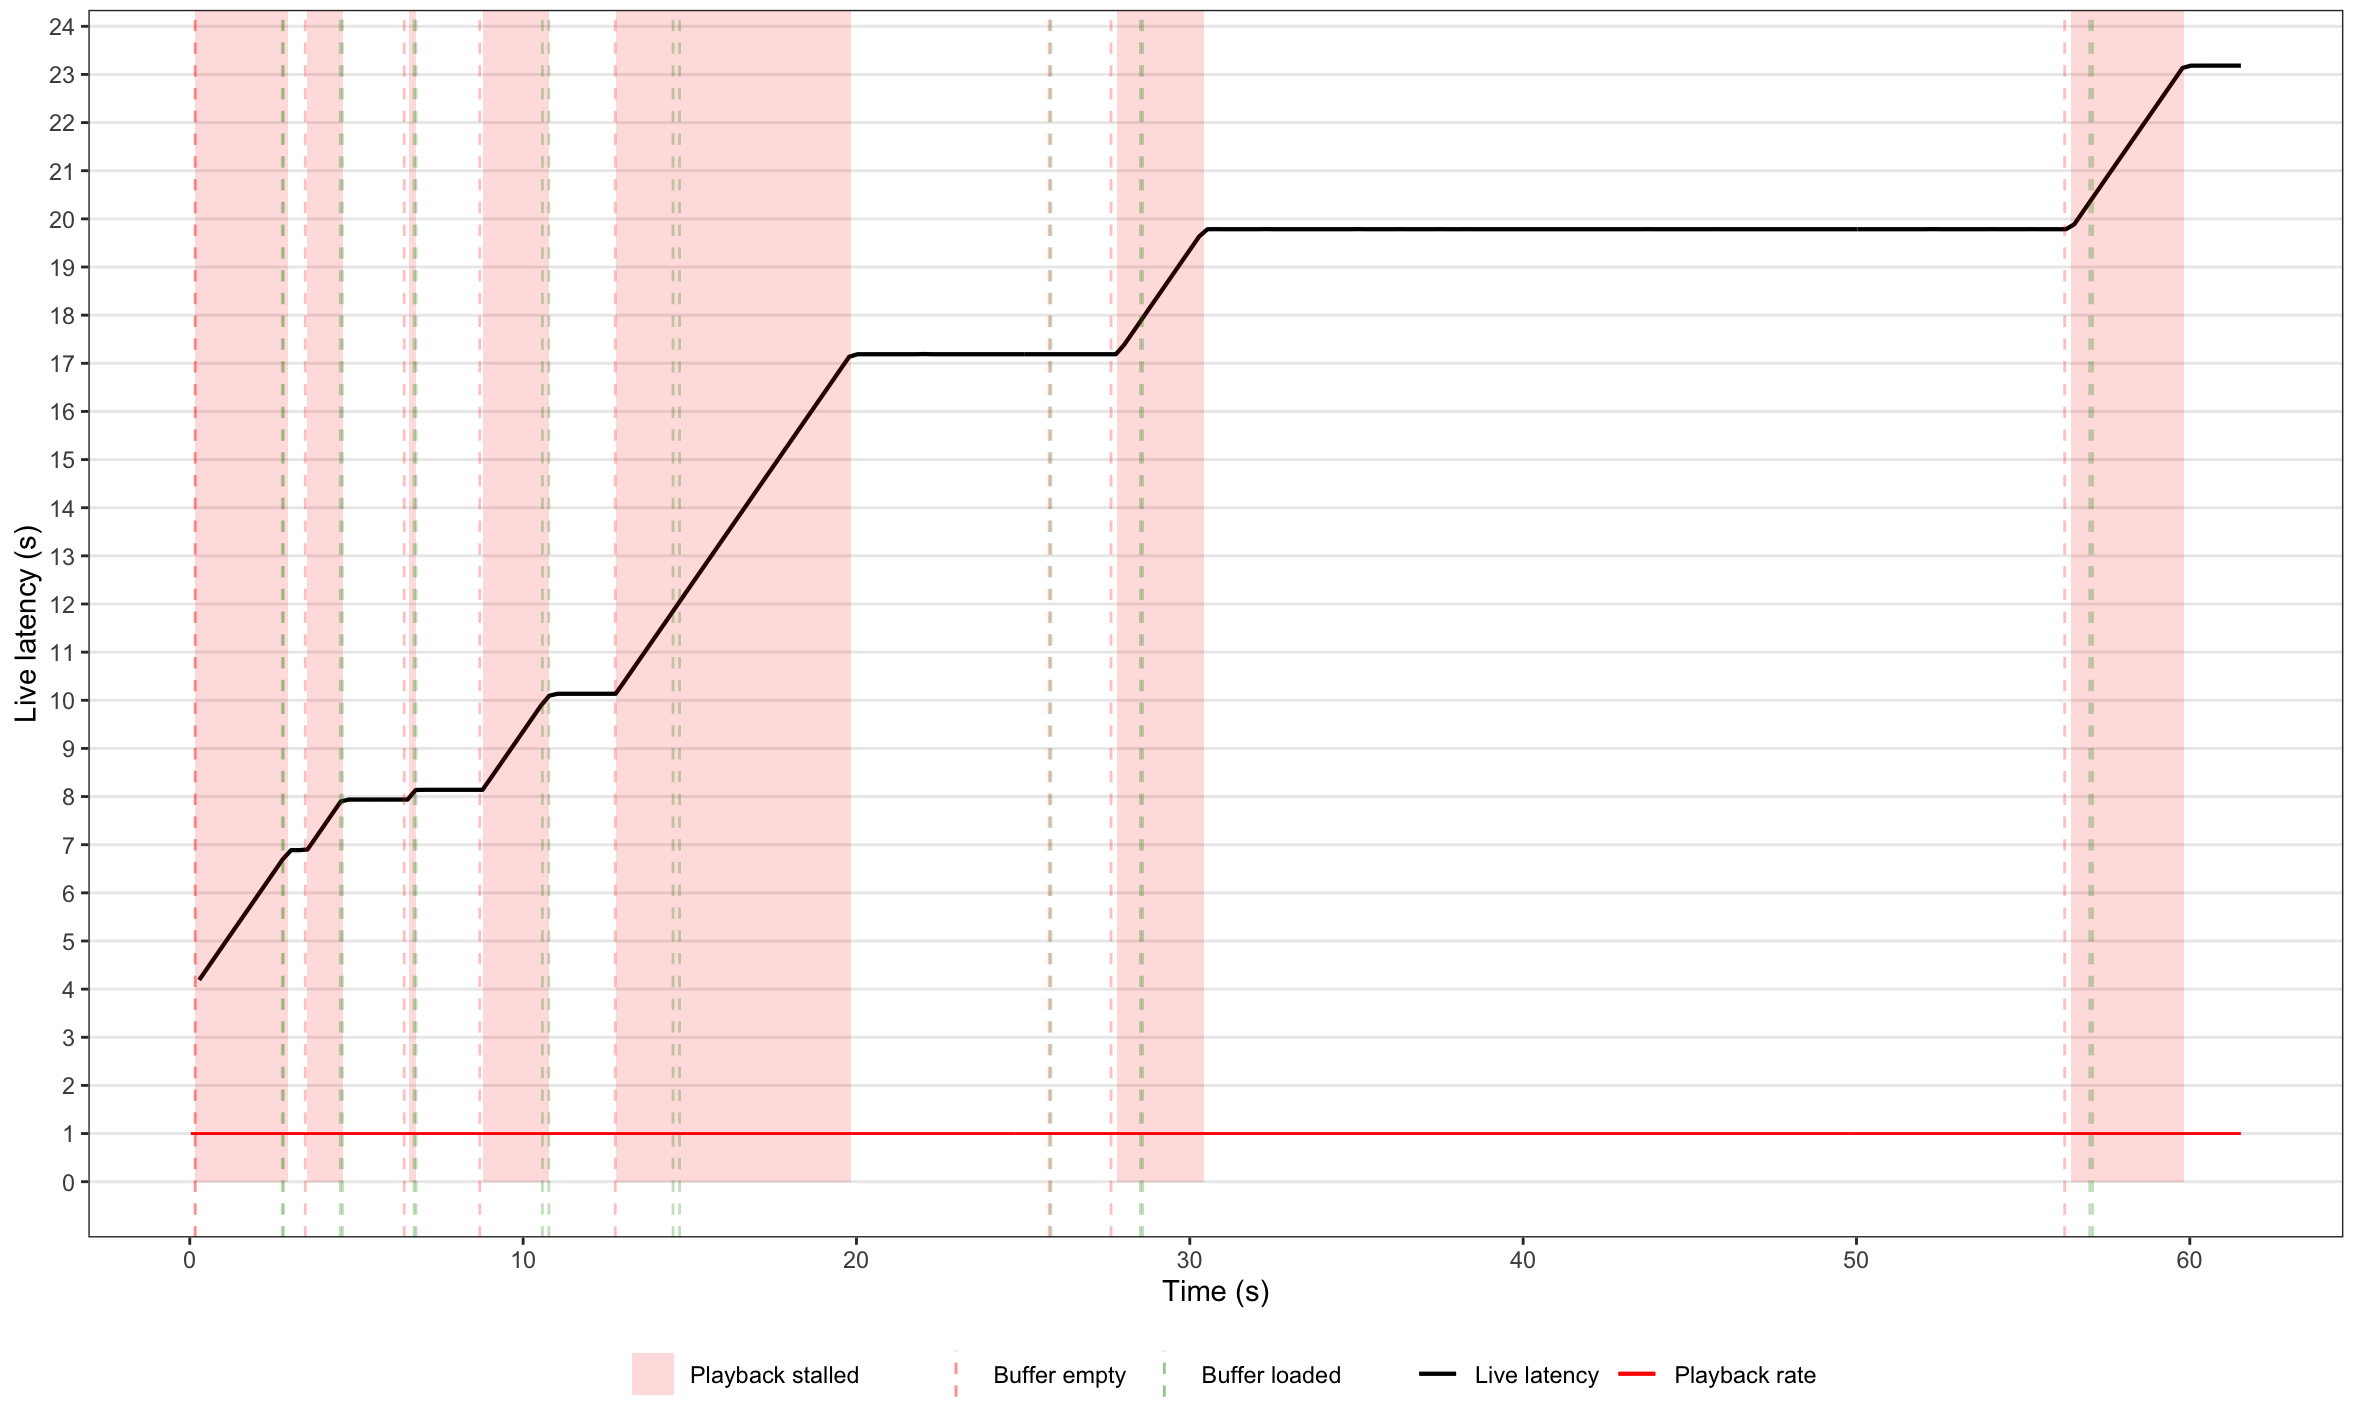
\includegraphics[width=\textwidth]{res/eval_nonabr_hspa+_h3_latency.png}
		\caption{Caption}
		\label{fig:eval_nonabr_hspa+_h3_waterfall}
	\end{subfigure}
	
	\caption{Caption}
	\label{fig:eval_nonabr_hspa+_h3}
\end{figure}

\textbf{Adaptive bitrate streaming} is needed for this reason: when the adaptation algorithms estimate that there is not enough bandwidth to continue the playback at the current bitrate, it will make the decision to switch to a lower bitrate. In the next sections, we will see how the system performs when adaptive bitrate streaming is enabled.

\subsection{Experiments and results in an ABR setup}
\label{sec:eval/abr}

The testbed that we introduced in Section \ref{sec:eval/testbed} is already capable of running experiments on an adaptive live stream. In fact, if we do not specify the minimum bitrate in the experiment configuration, the playback will use ABR. We tested this setup with both DASH.js and hls.js.

\subsubsection{Suboptimal behavior of the default DASH.js configuration with live}
\label{sec:eval/abr/dashjs}

An experiment we ran involved using DASH.js with the ABR stream and the \texttt{lte} network pattern. As a reminder, the bitrate ladder we are using in this experiment is made of four resolutions (720p, 540p, 360p, 270p) with video bitrates of 3.5 Mbps, 2.5 Mbps, 1.5 Mbps and 0.8 Mbps.

The buffer health plot in Figure \ref{fig:eval_abr_dashjs} shows that with this configuration buffer underflows and playback stalls are essentially eliminated, compared to Figure \ref{fig:eval_nonabr_lte_h3} (non-ABR case) where there were multiple stalls. This is due to the fact that the default configuration of DASH.js is relatively aggressive in downswitching the resolution/bitrate. Therefore, it is able to quickly react to the worsening network conditions at about 30 seconds, and lower the bitrate to 2.5 and then 1.5 Mbps. A similar result (not shown here) is obtained with the \texttt{hspa+} pattern.

\begin{figure}[h]
    \centering
    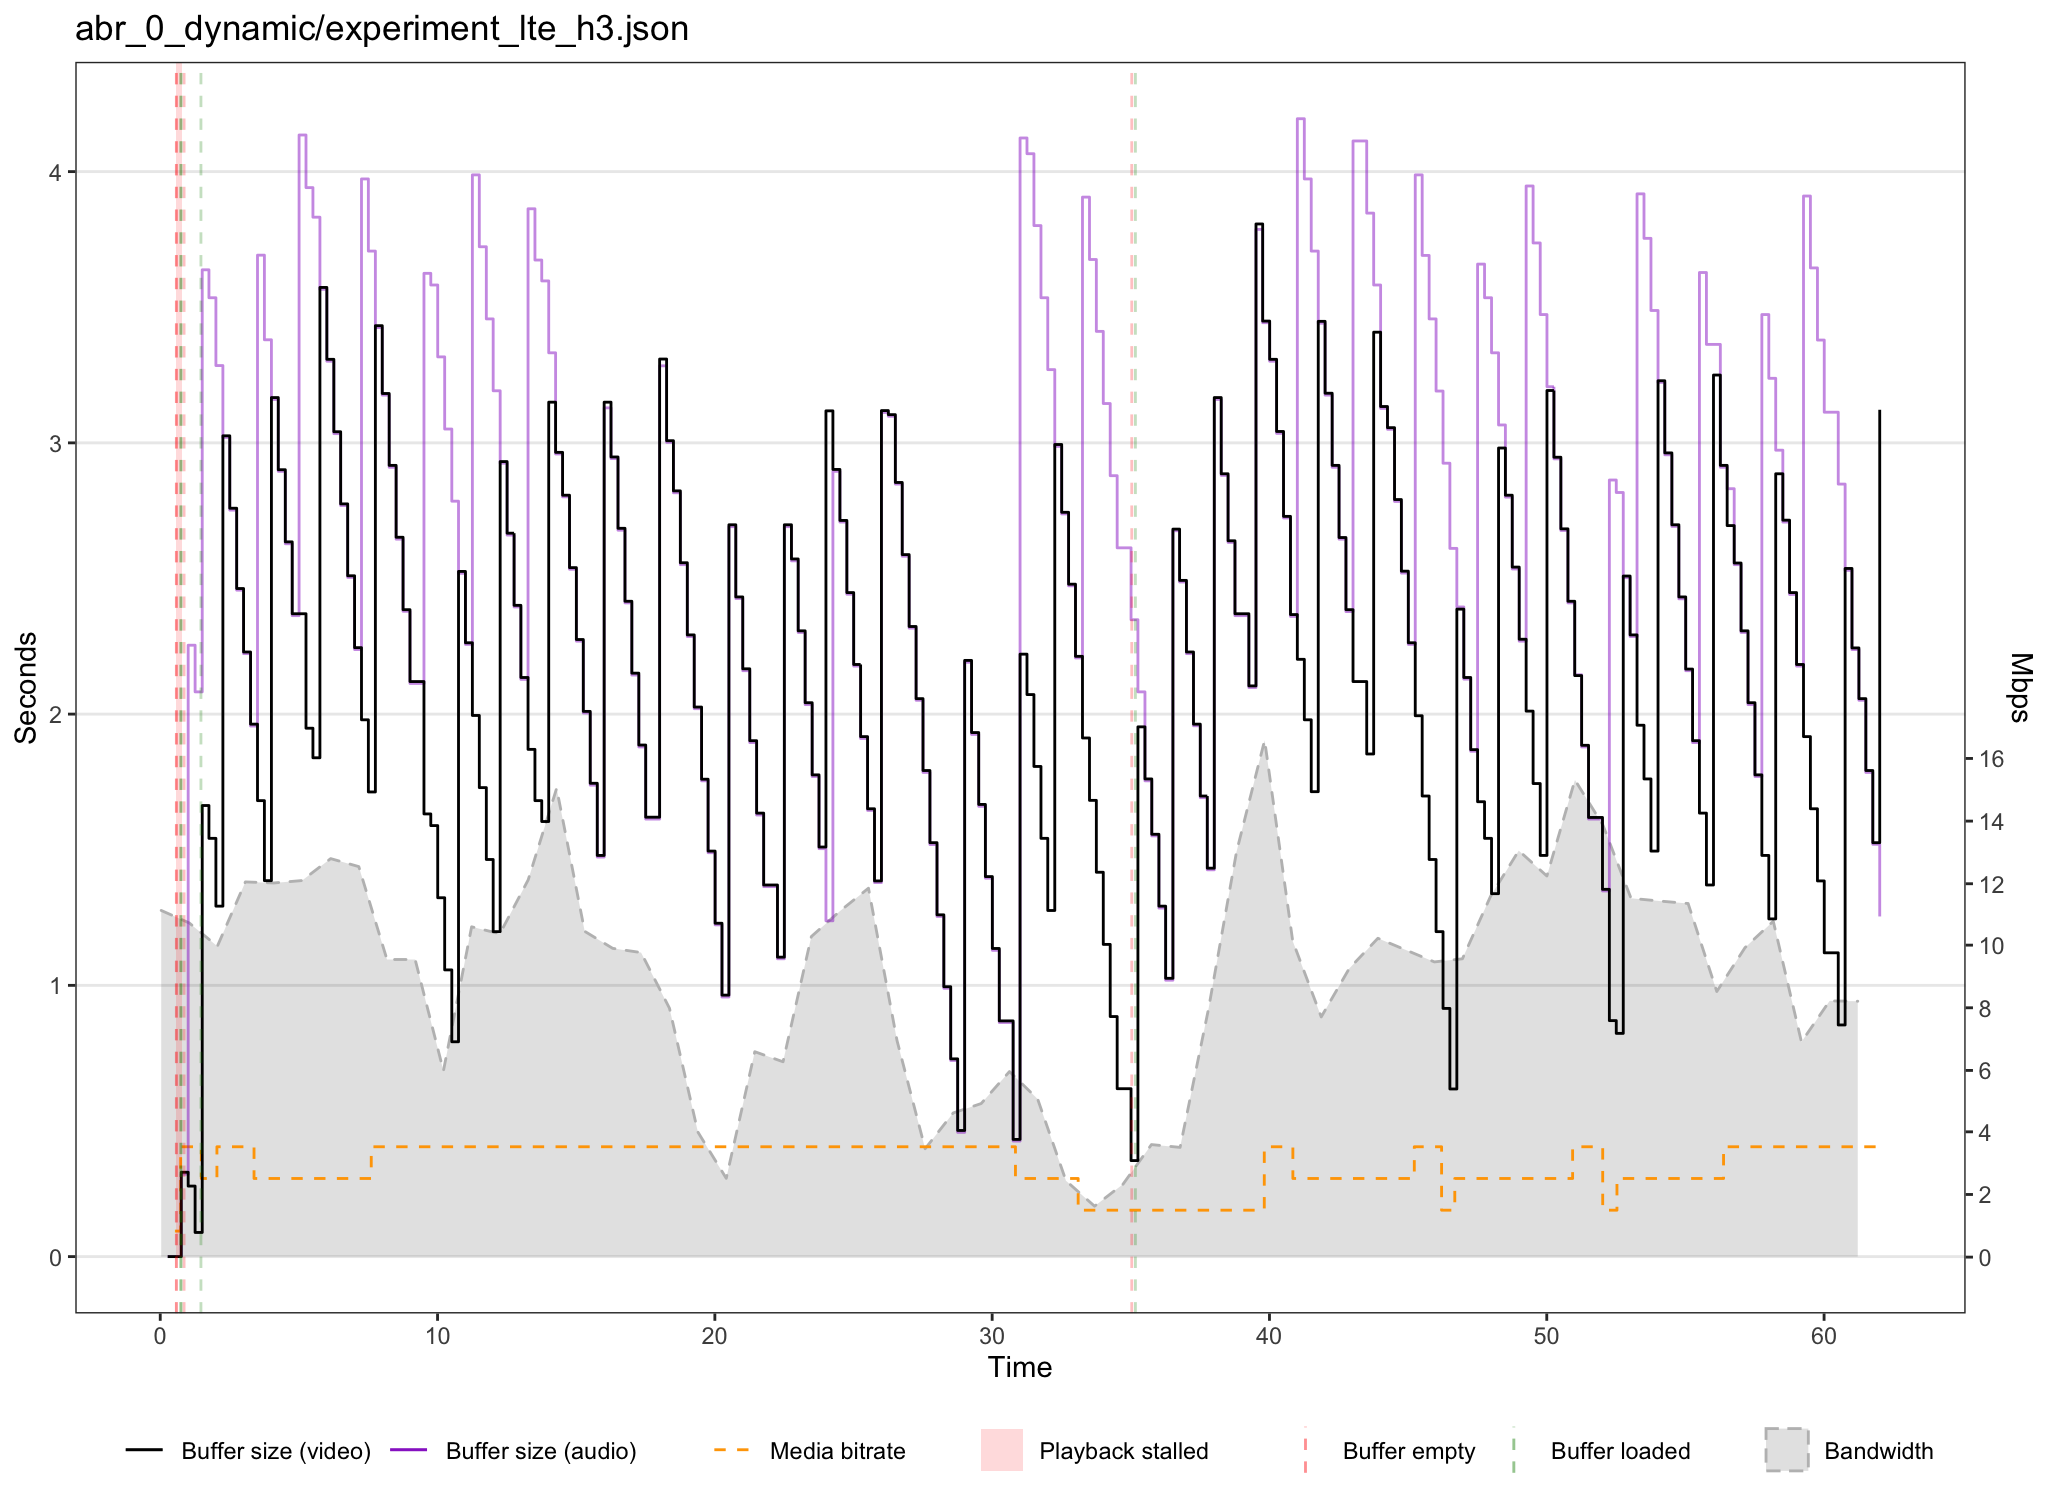
\includegraphics[width=0.9\textwidth]{res/eval_abr_dash_dynamic.png}
    \caption{Caption}
    \label{fig:eval_abr_dashjs}
\end{figure}

There is, however, an evident disadvantage to this aggressive approach, which can be seen between second 40 and second 60 in the plot. The bandwidth is always above 8 Mbps in that interval of the experiment, and thus there should be more than enough bandwidth to keep the stream at the highest quality and bitrate (3.5 Mbps).

Instead, what we observe is that the adaptation algorithm keeps switching quality in a way that does not seem to make much sense. At second 40, the bitrate is raised to 3.5 Mbps but almost immediately switched down to 2.5 Mbps. The algorithm then tries to raise the bitrate again and immediately falls to 1.5 Mbps. This oscillating pattern is repeated a few times until the experiment is over.

We observed that this behavior is consistent between different runs of the same experiment and is therefore something that should be investigated.

% TODO: try both dash and hls with hspa+

\subsubsection{Other network patterns and experiments with hls.js}
\label{sec:eval/abr/hls}

To find a situation where the adaptation algorithm does not behave well and leads to playback stalls, we relied on new network patterns inspired by Twitch's dataset for low-latency scenarios, introduced in \ref{sec:eval/testbed/network/patterns}. Specifically, for this analysis we will take into consideration the \texttt{spike} pattern, which contains an abrupt drop in bandwidth that lasts for a few seconds. The duration of the experiments based on this pattern is about 30 seconds.

At this point of the analysis, we also had a complete implementation of the integration with hls.js in the testbed, and therefore we ran the experiments with both DASH.js and hls.js.

Figure \ref{fig:eval_abr_hls} shows the buffer health plot of an experiment run with hls.js and the \texttt{spike} network pattern over HTTP/3. As can be seen, when the bandwidth suddenly drops from about 4 to 1 Mbps, the adaptation algorithm struggles to react in time, causing a couple of playback stalls and thus increasing latency. An observation we could make is that if the audio had priority over video, the playback stalls would be avoided since the stalls are shorter than 3 seconds. Section X will show how this can actually be implemented.

\begin{figure}[h]
    \centering
    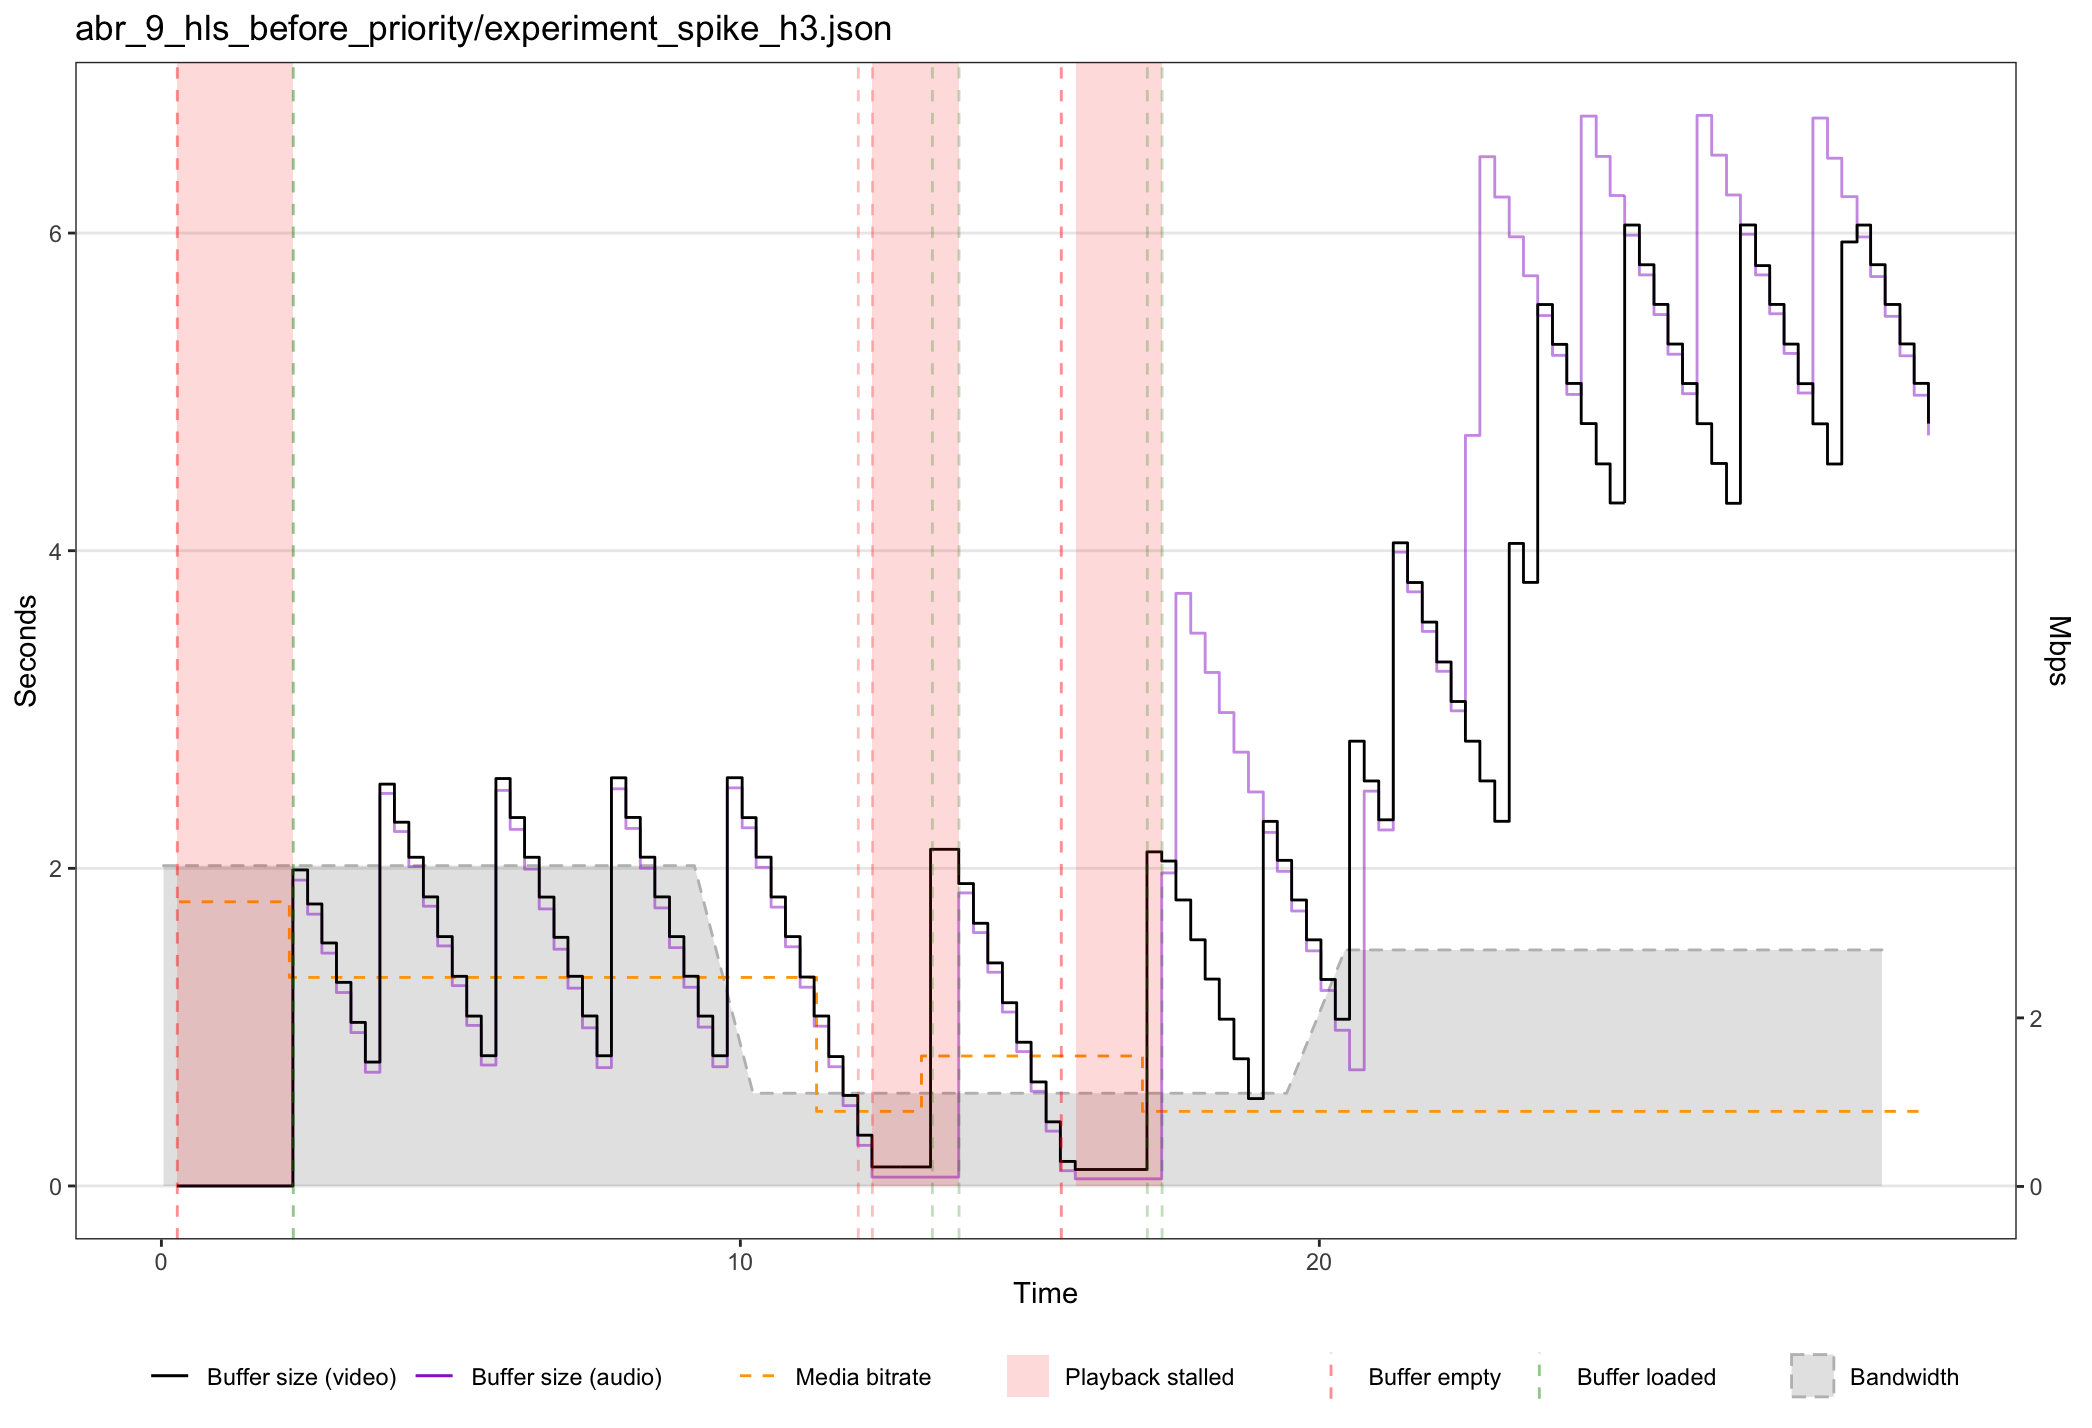
\includegraphics[width=0.9\textwidth]{res/eval_abr_spike_hls.png}
    \caption{Caption}
    \label{fig:eval_abr_hls}
\end{figure}

Finally, we also tested the behavior of the system when the live catchup feature is enabled. The live catchup feature increases the playback rate when the measured live latency is greater than the target one, up to a specified limit. In our tests, we used a maximum speed up of 1.5x. The results (not shown here) show that the live catchup indeed reduces the average latency, however seemingly causing additional playback stalls. The other obvious disadvantage is that for many types of video content having an increased playback rate is not an ideal experience.



      
    \endgroup


    % bibliography - bibtex format
    %
    % add chapter to index
    \addcontentsline{toc}{chapter}{Bibliography}
    % alphabetical order of authors
    \bibliographystyle{plain}
    \bibliography{parts/biblio}


%% In the bibliography, all the sources consulted for the dissertation 
%% have to be cited and listed in alphabetical order by the 
%% first author's surname.
%%
%% According to the source material, the quotation has to be as follows:
%%
%% BOOKS
%% Surname and initial/s of the name/s of the author/s, date of edition,
%% publishing house and (if applicable) number of edition.
%% 
%% JOURNAL ARTICLES 
%% Surname and initial/s of the first name/s of the author/s,
%% title of the article, name of the journal, volume number, issue number
%% and page numbers.
%% 
%% CONFERENCE PAPERS
%% Surname and initial/s of the name/s of the author/s,
%% year of the conference, title of the article, name of the conference,
%% place of the conference, conference dates, page numbers.
%% 
%% CITING WEB RESOURCES
%% The consulted webpages have to be listed in alphabetical order. 
%% It is necessary to:
%%   - Copy the specific URL (the web address) of the consulted webpage
%%   - If available, indicate the surname and first name of the author/s,
%%     the title and subtitle of the text
%%   - If available, indicate the last date you retrieved the webpage
%%     (day/month/year).   
    

    \titleformat{\chapter}
        {\normalfont\Huge\bfseries}{Appendix \thechapter}{1em}{}
    % Appendix / attachment section - optional
    \appendix
    \chapter{Title first appendix}

Lorem ipsum dolor sit amet, consectetur adipiscing elit. Donec sed nunc orci. Aliquam nec nisl vitae sapien pulvinar dictum quis non urna. Suspendisse at dui a erat aliquam vestibulum. Quisque ultrices pellentesque pellentesque. Pellentesque egestas quam sed blandit tempus. Sed congue nec risus posuere euismod. Maecenas ut lacus id mauris sagittis egestas a eu dui. Class aptent taciti sociosqu ad litora torquent per conubia nostra, per inceptos himenaeos. Pellentesque at ultrices tellus. Ut eu purus eget sem iaculis ultricies sed non lorem. Curabitur gravida dui eget ex vestibulum venenatis. Phasellus gravida tellus velit, non eleifend justo lobortis eget. 

\section{Title}
Lorem ipsum dolor sit amet, consectetur adipiscing elit. Donec sed nunc orci. Aliquam nec nisl vitae sapien pulvinar dictum quis non urna. Suspendisse at dui a erat aliquam vestibulum. Quisque ultrices pellentesque pellentesque. Pellentesque egestas quam sed blandit tempus. Sed congue nec risus posuere euismod. Maecenas ut lacus id mauris sagittis egestas a eu dui. Class aptent taciti sociosqu ad litora torquent per conubia nostra, per inceptos himenaeos. Pellentesque at ultrices tellus. Ut eu purus eget sem iaculis ultricies sed non lorem. Curabitur gravida dui eget ex vestibulum venenatis. Phasellus gravida tellus velit, non eleifend justo lobortis eget. 

\subsection{Sub-title}
Lorem ipsum dolor sit amet, consectetur adipiscing elit. Donec sed nunc orci. Aliquam nec nisl vitae sapien pulvinar dictum quis non urna. Suspendisse at dui a erat aliquam vestibulum. Quisque ultrices pellentesque pellentesque. Pellentesque egestas quam sed blandit tempus. Sed congue nec risus posuere euismod. Maecenas ut lacus id mauris sagittis egestas a eu dui. Class aptent taciti sociosqu ad litora torquent per conubia nostra, per inceptos himenaeos. Pellentesque at ultrices tellus. Ut eu purus eget sem iaculis ultricies sed non lorem. Curabitur gravida dui eget ex vestibulum venenatis. Phasellus gravida tellus velit, non eleifend justo lobortis eget. 


\chapter{Title first appendix}

Lorem ipsum dolor sit amet, consectetur adipiscing elit. Donec sed nunc orci. Aliquam nec nisl vitae sapien pulvinar dictum quis non urna. Suspendisse at dui a erat aliquam vestibulum. Quisque ultrices pellentesque pellentesque. Pellentesque egestas quam sed blandit tempus. Sed congue nec risus posuere euismod. Maecenas ut lacus id mauris sagittis egestas a eu dui. Class aptent taciti sociosqu ad litora torquent per conubia nostra, per inceptos himenaeos. Pellentesque at ultrices tellus. Ut eu purus eget sem iaculis ultricies sed non lorem. Curabitur gravida dui eget ex vestibulum venenatis. Phasellus gravida tellus velit, non eleifend justo lobortis eget. 

\section{Title}
Lorem ipsum dolor sit amet, consectetur adipiscing elit. Donec sed nunc orci. Aliquam nec nisl vitae sapien pulvinar dictum quis non urna. Suspendisse at dui a erat aliquam vestibulum. Quisque ultrices pellentesque pellentesque. Pellentesque egestas quam sed blandit tempus. Sed congue nec risus posuere euismod. Maecenas ut lacus id mauris sagittis egestas a eu dui. Class aptent taciti sociosqu ad litora torquent per conubia nostra, per inceptos himenaeos. Pellentesque at ultrices tellus. Ut eu purus eget sem iaculis ultricies sed non lorem. Curabitur gravida dui eget ex vestibulum venenatis. Phasellus gravida tellus velit, non eleifend justo lobortis eget. 

\subsection{Sub-title}
Lorem ipsum dolor sit amet, consectetur adipiscing elit. Donec sed nunc orci. Aliquam nec nisl vitae sapien pulvinar dictum quis non urna. Suspendisse at dui a erat aliquam vestibulum. Quisque ultrices pellentesque pellentesque. Pellentesque egestas quam sed blandit tempus. Sed congue nec risus posuere euismod. Maecenas ut lacus id mauris sagittis egestas a eu dui. Class aptent taciti sociosqu ad litora torquent per conubia nostra, per inceptos himenaeos. Pellentesque at ultrices tellus. Ut eu purus eget sem iaculis ultricies sed non lorem. Curabitur gravida dui eget ex vestibulum venenatis. Phasellus gravida tellus velit, non eleifend justo lobortis eget. 




\end{document}
